\documentclass[degree=doctor]{ustcthesis}
% degree      = doctor | master | bachelor
% degree-type = academic | professional | engineering
% language    = chinese | english
% fontset     = windows | mac | ubuntu | fandol

% 加载宏包、全部的配置
\input{ustcsetup}

\newcommand{\va}{\boldsymbol{a}}
\newcommand{\vb}{\boldsymbol{b}}
\newcommand{\id}{\mathrm{id}}
\newcommand{\E}{\mathcal{E}}
\newcommand{\X}{\mathcal{X}}
\newcommand{\bE}{\boldsymbol{E}}
\newcommand{\pE}{\mathcal{E}_{*}}
\newcommand{\fE}{{}^{i}\E}
\newcommand{\bcE}{\boldsymbol{\mathcal{E}}}
\newcommand{\F}{\mathcal{F}}
\newcommand{\bF}{\boldsymbol{F}}
\newcommand{\pF}{\mathcal{F}_{*}}
\newcommand{\fF}{{}^{i}\F}
\newcommand{\bcF}{\boldsymbol{\mathcal{F}}}
\newcommand{\pS}{\mathcal{S}_{*}}
\newcommand{\Sb}{\mathcal{S}}
\newcommand{\G}{\mathcal{G}}
\newcommand{\bG}{\boldsymbol{G}}
\newcommand{\pG}{\mathcal{G}_{*}}
\newcommand{\fG}{{}^{i}\G}
\newcommand{\bcG}{\boldsymbol{\mathcal{G}}}
\newcommand{\T}{\mathcal{T}}
\newcommand{\U}{\mathcal{U}}
\newcommand{\ch}{\operatorname{ch}}
\newcommand{\cl}{\operatorname{c}}
\newcommand{\tr}{\operatorname{Tr}}
\newcommand{\cok}{\operatorname{coker}}
\newcommand{\rank}{\operatorname{rank}}
\newcommand{\Gr}{\operatorname{Gr}}
\newcommand{\Hom}{\operatorname{Hom}}
\newcommand{\dg}{\operatorname{deg}}
\newcommand{\diff}{\mathop{}\!\mathrm{d}}  % 正体微分d
\newcommand{\pdiff}{\mathop{}\!\mathrm{\partial}} 
\newcommand{\boplus}{\boldsymbol{\scalebox{1.3}{$\oplus$}}}
\newcommand{\wnabla}{\widetilde{\nabla}}
\newcommand{\wnablayl}{\widetilde{\nabla}^{1,0}}
\newcommand{\wnablaly}{\widetilde{\nabla}^{0,1}}
\newcommand{\iwnabla}{{}^{I}\!\widetilde{\nabla}}
\newcommand{\iwnablayl}{{}^{I}\!\widetilde{\nabla}^{1,0}}
\newcommand{\iwnablaly}{{}^{I}\!\widetilde{\nabla}^{0,1}}
\newcommand{\iPsi}{{}^{I}\!\Psi}
\newcommand{\iPsiyl}{{}^{I}\!\Psi^{1,0}}
\newcommand{\iPsily}{{}^{I}\!\Psi^{0,1}}
\newcommand{\Psiyl}{\Psi^{1,0}}
\newcommand{\Psily}{\Psi^{0,1}}
\newcommand{\g}{\mathfrak{g}}
\newcommand{\h}{\mathfrak{h}}
\newcommand{\kk}{\mathfrak{k}}
\newcommand{\Ad}{\operatorname{Ad}}
\newcommand{\GL}{\operatorname{GL}}
\newcommand{\Au}{\operatorname{Aut}}
\newcommand{\En}{\operatorname{End}}
\newcommand{\LL}{\operatorname{\mathcal{L}}}
\newcommand{\OX}{\operatorname{\mathcal{O}_X}}
\newcommand{\HH}{\mathbb{H}}
\newcommand{\PSU}{\operatorname{PSU}}
\newcommand{\R}{\mathbb{R}}
\newcommand{\C}{\mathbb{C}}
\newcommand{\Div}{\operatorname{Div}}

\begin{document}

\maketitle
\copyrightpage

\frontmatter
% !TEX root = ../main.tex

\begin{innovations}

本论文研究了紧 Kähler 流形上带有除子奇性的向量丛及其推广对象的几何结构，主要关注抛物向量丛与 Hermitian--Einstein 度量之间的关系，并在此基础上讨论了 Kobayashi--Hitchin 对应在更一般情形下的成立问题。围绕这一主题，本文在现有理论基础上进行了若干推广和改进，主要创新性体现在以下几个方面。

首先，本文在传统抛物向量丛理论的框架下，将研究对象推广到饱和自反抛物层，并在适当的稳定性条件下建立了其与 Hermitian--Einstein 度量之间的对应关系。已有的 Kobayashi--Hitchin 对应主要针对光滑情形或向量丛情形，而对于存在奇性结构的自反层情形，相关理论仍不完善。本文通过对奇性解析结构的细致分析，构造了适合自反抛物层的解析框架，从而将经典对应推广到更一般的几何对象。

其次，本文结合 Hironaka 奇点解析理论，对带有奇性结构的抛物层进行适当的解析化处理，并在解析化空间上建立了 Hermitian--Einstein 度量存在性的分析方法。通过在解析化后的空间上构造适当的度量和连接，并利用椭圆型偏微分方程的估计方法，本文给出了 Hermitian--Einstein 方程在奇性背景下的可解性分析，从而为建立对应关系提供了关键的解析工具。

再次，本文在上述结构基础上进一步研究了相关的 Chern 类与稳定性之间的关系，得到了一类 Bogomolov--Gieseker 型不等式。这一不等式为抛物自反层的稳定性提供了必要的数值条件，同时也为研究其模空间结构提供了重要的几何约束。

综上所述，本文在抛物几何与 Hermitian--Einstein 度量理论的交叉研究中，对带奇性几何对象的 Kobayashi--Hitchin 对应进行了系统研究，并在解析方法和几何结构方面给出了一定的推广与补充，为进一步研究带奇性结构的复几何对象提供了新的思路和工具。


\end{innovations}


% \begin{innovations}
%
% 工程博士学位论文应主要聚焦工程实践和应用研究，须体现工程性、创新性、实践性、应用性特征，
% 体现学位申请人在专业领域掌握坚实全面的基础理论和系统深入的专门知识，
% 具有独立承担专业实践工作的能力，在专业实践领域做出创新性成果，
% 对推动本专业领域知识和技术的发展作出重要贡献。
%
% 故在此须说明本学位论文的创新性及应用性，确保符合工程博士学位论文要求，字数在800字以内。
%
% \end{innovations}
  % 博士学位论文的创新性说明
% !TEX root = ../main.tex

\ustcsetup{
  keywords  = {Kobayashi--Hitchin 对应，抛物层，Hermitian--Einstein 度量，Bogomolov--Gieseker 不等式},
  keywords* = {Kobayashi--Hitchin correspondence, parabolic sheaves, Hermitian--Einstein metrics, Bogomolov--Gieseker inequality},
}

\begin{abstract}

本文研究了紧 Kähler 流形上带有光滑除子的抛物结构，并在此背景下讨论饱和自反抛物层的 Kobayashi--Hitchin 对应问题。通过结合 Hironaka 奇点解析理论，对具有奇性结构的层进行适当的解析化处理，并在解析空间上构造适合的 Hermitian 度量与连接，然后利用 Hermitian--Yang--Mills 流说明在适当的稳定性条件下，饱和自反抛物层与 Hermitian--Einstein 度量之间的对应关系，从而将经典 Kobayashi--Hitchin 对应推广到更一般的几何情形。

此外，本文进一步研究了相关向量丛与自反层的 Chern 类性质，并在此基础上建立了一类 Bogomolov--Gieseker 型不等式。



\end{abstract}

\begin{abstract*}
  
  In this thesis, we study parabolic structures along smooth divisors on compact Kähler manifolds and investigate the Kobayashi--Hitchin correspondence for saturated reflexive parabolic sheaves. By combining techniques from Hironaka's resolution of singularities with analytic methods in complex differential geometry, we construct an appropriate analytic framework for dealing with singular geometric structures. In particular, we establish the existence of Hermitian--Einstein metrics under suitable stability conditions and prove a Kobayashi--Hitchin type correspondence for saturated reflexive parabolic sheaves.

  Furthermore, we analyze the behavior of Chern classes associated with such sheaves and derive a Bogomolov--Gieseker type inequality.


\end{abstract*}

\tableofcontents
% \listoffigures
% \listoftables
% \listoffiguresandtables
% \include{chapters/notation}

\mainmatter
% !TEX root = ../main.tex



\chapter{预备章节}
\section{K\"ahler 流形}
一个Hermitian流形$(X,g)$是一个复流形$X$配上一个和其复结构$I$相容的黎曼度量$g$，相容即是指
\[
g(\cdot,\cdot)=g(J(\cdot),J(\cdot))
\]
将$X$看成实流形我们将其切丛记为$T_X$，其复化被复结构分裂成
\[
T_X\otimes \C=T^{1,0}\oplus T^{0,1}
\]
特别的$(T_X,I)$与$T^{1,0}$存在自然同构
\[ 
v\to \frac{1}{2}(v-iI(v))
\]
相对应的，对于复化的$k$-形式丛我们有
\[
\Omega_X^k=\bigoplus_{p+q=k}\Omega_X^{p,q}
\]
$g$可以诱导一个$(1,1)$-形式$\omega\coloneqq g(I(\cdot),\cdot)$。若$\omega$是闭形式，则称$(X,g)$为K\"ahler流形。由于$\omega$可以还原出$g$，我们也可将其记为$(X,\omega)$。

同时$g$可以诱导出$(T_X,I)$上的Hermitian度量
\[
h\coloneqq g-i\omega
\]
我们将$g$的复化记为$g_{\C}$，需注意，将其限制在$T^{1,0}$上我们有
\[g_{\C}=\frac{1}{2}h\]
在局部坐标$z=(z^1,\cdots,z^n)$下，我们有
\[
h=h_{i\bar{j}}\diff z^i\otimes \diff \overline{z}^j\quad \omega=\frac{i}{2} h_{i\bar{j}}z^i\otimes \diff \overline{z}^j
\]

在$\Omega_X^\bullet$上，我们定义Lefschetz算子$L\coloneqq \cdot\wedge \omega$。
由于$g_{\C}$诱导了$\Omega_X^\bullet$上的内积，我们有自然的伴随算子，将其记为$\Lambda$。在局部坐标下若有$(1,1)$-形式$\eta=\eta_{i\bar{j}}dz^i\wedge d\overline{z}^j$，我们有
\[
\Lambda\eta=\frac{2}{i}h^{\bar{i}j}\eta_{i\bar{j}}
\]
特别的对于光滑函数$f$，
\[
-2i\Lambda \partial\overline{\partial}f=\Delta_g f \footnote{在本篇文章中，我们约定Laplace算子为$\Delta=-\Div\cdot \nabla f$。}
\]

\section{抛物丛起源}
全纯向量丛上的抛物结构最早应出自\cite{Me-Se}。文章作者通过研究平坦向量丛在非紧黎曼面上的无穷远渐进行为获得了抛物结构。本小节将简单介绍抛物结构的来源以及定义抛物结构的动机。

令 $G\subset \PSU(2,\R)$ 是一个离散子群，使得它自由地作用于上半平面$\HH$且其商空间是有限体积的。令$\HH^+=P\cup \HH$其中$P$为群作用的抛物点，则$X=\HH^+/G$是一个紧黎曼面。给定一个$n$维厄米特向量空间$V$以及一个酉表示$\rho: G\to \GL(n,V)$, 我们得到一个带$G$作用的向量丛$E=\HH\times V$. 我们总是可以通过共轭变换将抛物点变到无穷远点，因此我们只考虑抛物点为无穷远点的情况。令$y\in P$ 是$X$上的一个抛物尖点，则对于$\delta$充分大，存在一个邻域$\U_y=\HH_\delta/G_\infty$, 其中$\HH_\delta\coloneqq \{z=x+iy\in \HH|y>\delta\}$, $G_\infty$由一个抛物元素$T:z\mapsto z+a$生成，其中$a\in \R$，为简单起见我们取$a=1$。

由以上设定，我们考虑丛$E$限制在$\HH_\delta$上的$G$不变的有界全纯截面，即有界全纯映射$F:\HH^+_\delta\to \HH^+_\delta\times V$其形式为$F(z)=(z,f(z))$并且满足$f(z+1)=\rho(T)\cdot f(z)$. 在合适的酉标架$\{e_i\}_i$下，$\rho(T)$可以被对角化为
\[
\rho(T)=
\begin{pmatrix*}
    \exp(2\pi i \alpha_1) & &\\
    & \ddots & \\
    & & \exp(2\pi i \alpha_n)
\end{pmatrix*}
\]
其中$0\leq \alpha_i\leq\alpha_{i+1}<1$。则在该酉标架下$f=(f_i)_i$满足$f_i(z+1)=\exp(2\pi i \alpha_i)f_i(z)$，通过直接计算可得$f_i(z)=\exp(2\pi i \alpha_i z)g_i(\tau)$ 其中$\tau=\exp(2\pi i z)$, $g_i$ 是去心圆盘上的全纯函数。由于$f$是有界的，因此$g_i$在$\tau=0$处也是全纯的。

基于以上观察，我们可以在紧黎曼面$X$上定义局部自由层$\pE$，其定义如下：我们把$\HH^+$到$X$的商映射记成$q$, 对于不与抛物点相交的开集$\U$，$\pE(\U)=E^G(q^{-1}(\U))$, 其中$E^G$表示$G$不变的全纯截面。对于包含抛物点$y$的开集$\U_y$, $\pE(\U_y)$则由上述讨论的$G$不变的有界全纯截面组成。上述讨论表明，${\pE}_{,y}$ 是秩为$n$的${\OX}_{,y}$自由模，其生成元为$F_i: z\to \exp(2\pi i \alpha_i z)e_i$，因此$\pE$是局部自由层，我们也可以认为$\pE$是紧黎曼面$X$上的向量丛。

基于$V$上的度量，我们有$|F_i|=O(|\tau|^{-\alpha_i})$，因此我们可以基于这些生成元的收敛速度在$y$处对该向量丛的纤维$W_y$进行分层。将互不相同的$\alpha_i$从小到大记为$\{\alpha_j\}_j$, 令$F_jW_{y}\coloneqq\{F_i||F_i|\geq |\tau|^{-\alpha_j}\}$，我们得到一个递减的滤链
\[
 W_y=F_1W_{y}\supset F_2W_{y}\supset \cdots \supset F_lW_{y}\supset F_{l+1}W_{y}=0
\]
对于每个$F_jW_y$我们赋予权重$\alpha_j$, 从而得到一个带权的滤链。
我们称该带权滤链为向量丛$\pE$在$y$处的抛物结构。对于包含多个抛物点的情况，我们可以在每个抛物点处定义类似的滤链，从而得到一个全局的抛物结构。

引入抛物结构的目的在于记录原始向量丛$E$在无穷远点处的渐近行为，从而尽可能多的保留原始向量丛$E$的信息。事实上，我们有以下结论：
\begin{proposition}
    假设$E_1$，$E_2$是来自如上所述的两个$G$的酉表示产生的向量丛，则他们各自诱导抛物丛${\pE}_1$，${\pE}_2$。对任意的$G$等变态射$\phi: E_1 \to E_2$，它诱导了丛${\pE}_1$到${\pE}_2$的态射，不妨依旧记为$\phi$，并且在抛物点$y$处满足$\phi(F_iW_{1,y})\subset F_jW_{2,y}$当且仅当$\alpha_{1,i}>\alpha_{2,j}$。
\end{proposition}
因此记录抛物结构是有必要的。

以上的内容成为了抛物丛定义的动机。
% \section{脚注}
\section{Hodge丛}
由于本篇文章极大地受到了Simpson~\cite{Si1}的启发，在本预备章节的最后我们重新回顾~\cite{Si1}当中的结果。
\subsection{Hodge结构的形变}
考虑 $\phi: Y \to X$ 是一个极化 Kähler 流形的族。即存在 $\omega \in H^2(Y, \mathbb{Z})$，使得对于任意 $x \in X$，$\omega|_{Y_x}$ 是 Kähler 的。

在局部 $U_x \subset X$ 上，$Y$ 微分同胚于 $Y_x \times U_x$。考虑向量丛 $R^k\phi_* \mathbb{C} \otimes \mathcal{O}_X|_{U_x} \simeq H^k(Y_x, \mathbb{C}) \times U_x$。在此之上存在 Gauss-Manin 联络 $\nabla = d$。对于任意两根纤维 $H^k(Y_x, \mathbb{C}) \simeq H^k(Y_{x'}, \mathbb{C})$（通过基于 $\nabla=d$ 的平行移动诱导同构）。

Lefschetz 分解 $L: R^k\phi_* \mathbb{C} \xrightarrow{\cup [\omega]} R^{k+2}\phi_* \mathbb{C}$ 使得我们可以关注本原部分：
\[ R^k\phi_*\mathbb{C}_{\text{prim}} \otimes \mathcal{O}_X |_{U_x} \simeq H^k(Y_x, \mathbb{C})_{\text{prim}} \times U_x \]
在 $H^k(Y_x, \mathbb{Z})$ 上定义 $Q(\alpha, \beta) = <L^{n-k}\alpha, \beta>$，这与 $H^k(Y_x, \mathbb{Z}) \simeq H^k(Y_{x'}, \mathbb{Z})$ 的同构是兼容的。
因此，在向量丛 $R^k\phi_* \mathbb{C}_{\text{prim}} \otimes \mathcal{O}_X =: \mathcal{H}^k$ 上我们有一个 Hermitian 形式 $h(\alpha, \beta) \coloneqq i^{k} Q(\alpha, \bar{\beta})$，其关于 $\nabla$ 平行。

Hodge过滤 (Hodge filtration) 定义为 \[F^p H^k(Y_x, \mathbb{C}) = \oplus_{a \ge p} H^{a, k-a}(Y_x) \subset H^k(Y_x, \mathbb{C})\]
这给出了一个映射（局部）：
\[ \mathcal{P}^{k,p}: X \to G \subset \text{Gr}(k, p, H^k(Y_x, \mathbb{C})) \quad \text{(全纯)} \]
通过 $\mathcal{P}^{k,p}$ 拉回 $G$ 上的重言子丛 $S^{k,p}$，得到 $\mathcal{H}$ 的一个全纯子丛 $F^p\mathcal{H}$。

\textbf{Griffiths 横截性 (Griffiths transversality):}
\[ \nabla F^p \mathcal{H}^k \subset F^{p-1}\mathcal{H}^k \otimes \Omega_X^1 \]
这一性质诱导了一个全纯态射（无穷小 VHS 或 Higgs 场）：
\[ \theta: \mathcal{H}^{p,q} \to \mathcal{H}^{p-1, q+1} \otimes \Omega_X^1 \]
其中
\[
\mathcal{H}^{p,q} = F^p\mathcal{H}^k / F^{p+1}\mathcal{H}^k \simeq F^p\mathcal{H}^k \cap \overline{F^{k-p}\mathcal{H}^k}
\]
Griffiths 横截性给出了分解 $\nabla = \bar{\theta}_h + \partial_h + \bar{\partial} + \theta$。

\begin{definition}[极化Hodge结构 PVHS]
一个 PVHS 是一个 $C^\infty$ 丛 $(\oplus \mathcal{H}^{p,q}, \nabla)$ 存在Hermitian形式 $s = \oplus s^{p,q}$ （使得 $h = \oplus (-1)^p s^{p,q}$ 为度量），满足 $\nabla s = 0$。
\end{definition}

\begin{definition}[Hodge 丛系统]
一个 Hodge 丛系统是 $\oplus (\mathcal{H}^{p,q}, \bar{\partial})$ 配备 $\theta: \mathcal{H}^{p,q} \to \mathcal{H}^{p-1, q+1} \otimes \Omega_X^1$，满足 $\theta \wedge \theta = 0$（即无穷小 VHS）。
\end{definition}

\subsection{分析结果}

\begin{theorem}\label{th1}
假设 $(X, \omega)$ 满足 Simpson~\cite[Section 2]{Si1}的假设，且 $(E, \bar{\partial}, \theta, A, K)$ 是一个带有群作用 $A$ 和度量 $K$ 的 Higgs 丛，使得 $\Lambda F_{\nabla_K^{hs}}$ 有界，并且关于该群作用是稳定的。那么存在一个 $A$-不变度量 $H$，满足 $\det(H) = \det(K)$，与 $K$ 可比，$\bar{\partial}(K^{-1}H) \in L^2$，使得 $\Lambda F_{\nabla_H^{hs}}^\perp = 0$。
\end{theorem}

\begin{proposition}\label{prop3.3}
假设 $E$ 是一个 Higgs 丛，且 $H$ 是一个满足 $\Lambda F_{\nabla_H^{hs}}^\perp = 0$ 的度量。则
\[ \left( 2c_2(E, H) - \frac{r-1}{r} c_1(E, H)^2 \right) \cdot \omega^{n-2} = C \int_X \tr(F_{\nabla_H^{hs}}^\perp \wedge F_{\nabla_H^{hs}}^\perp) \wedge \omega^{n-2} \ge 0 \]
如果等号成立，则 $F^\perp = 0$。特别地，如果 $\tr(F)=0$ 且 $c_2(E, H) \cdot \omega^{n-2} = 0$，则 $\nabla_H^{hs}$ 是平坦的。
\end{proposition}

\subsection{VHS 的构造（向量丛版本）}

给定 $X$ 上的 Hodge 丛系统 $(\oplus_{p+q=k} \mathcal{H}^{p,q}, \theta)$，使得
\[ \theta: \mathcal{H}^{p,q} \to \mathcal{H}^{p-1, q+1} \otimes \Omega_X^1 \]
满足可积性条件 $\theta \wedge \theta = 0$，以及一个度量 $h = \oplus_{p+q=k} h^{p,q}$，我们可以构造一个 Hitchin-Simpson 联络 $\nabla_h^{hs} := \nabla_h^c + \theta + \theta^{*h}$，其中 $\nabla_h^c$ 是 $h$ 的 Chern 联络。
容易验证 $\nabla_h^{hs}$ 保持半双线性形式 $s := \oplus_{p+q=k} \sqrt{-1}^{q-p} h^{p,q}$。因此，如果曲率 $F_{\nabla_h^{hs}}$ 为零，我们就恢复了一个极化Hodge结构形变。

\begin{theorem}\label{th8.2}
假设 $(X, \omega)$ 是紧致 Kähler 流形。则Hodge结构形变的范畴（态射保持联络）同构于满足 $c_1(E)=0, c_2(E) \cdot [\omega]^{n-2} = 0$ 且为度数为零的稳定 Hodge 丛系统的直和的全子范畴。
\end{theorem}

\begin{proof}
如果 $E$ 是稳定且度数为零的，由 $\partial\bar{\partial}$-引理，我们可以在 $\det(E)$ 上找到一个度量 $h$ 使得 $F_{\nabla_h^{hs}}$ 是 $c_1(E)$ 的调和代表元，于是 $\Lambda F_{\nabla_h^{hs}} = 0$（注意对于线丛，Hitchin-Simpson 联络和 Chern 联络相同）。根据定理\ref{th1}，我们在 $E$ 上得到一个度量使得 $\Lambda F = 0$。如果 $E$ 在全子范畴中，我们对每个直和项做此操作。通过构造，$\tr(F)$ 是 $c_1(E)$ 的调和代表元，因此 $\tr(F)=0$。此时应用命题~\ref{prop3.3} 得到 $F=0$，即 $E$ 来自于一个Hodge结构形变。另一方面，如果 $E$ 来自 VHS，由 Chern-Weil 公式可知 $E$ 位于该子范畴中。

至此我们证明了该函子是满射。接下来证明它是全忠实的，即证明 VHS 范畴中的态射与 Hodge 丛系统范畴中的态射一一对应。单射是显然的，只需证明如果 $f: E' \to E''$ 是一个来自 VHS 范畴的 Hodge 丛系统映射，即 $E'$ 和 $E''$ 分别配备平坦联络 $\nabla'$ 和 $\nabla''$，则 $\nabla(f)=0$（其中 $\nabla$ 是 $\text{Hom}(E', E'')$ 上的诱导联络），或等价地 $f$ 保持联络。此处省略证明。实际上这是一个同构。假设从一个 VHS $(E, \nabla')$ 出发，使用定理\ref{th1} 得到 $E$ 上的平坦联络 $\nabla''$，上述论证表明 $\id: (E, \nabla') \to (E, \nabla'')$ 保持联络，即 $\nabla' = \nabla''$，因此它是同构。
\end{proof}

\subsection{VHS 的构造（主丛版本）}

\subsubsection*{Cartan 分解}

设 $\g_0$ 为实半单李代数，$\g$ 为其复化。$\g_0$ 的 Cartan 对合 $\theta$ 是一个对合自同构，使得双线性形式 $B_\theta(X, Y) := -B(X, \theta(Y))$ 是正定的，其中 $B$ 是 Killing 形式。我们有 Cartan 分解 $\g_0 = \mathfrak{k}_0 \oplus \mathfrak{p}_0$，其中 $\mathfrak{k}_0$ 和 $\mathfrak{p}_0$ 分别是 $\theta$ 特征值为 1 和 -1 的特征空间。复化后得到 $\g = \mathfrak{k} \oplus \mathfrak{p}$。

定义 $\tau := \sigma \circ \theta$，其中 $\sigma$ 是 $\g$ 关于 $\g_0$ 的复共轭。则 $h(X, Y) := -B(X, \tau(Y))$ 是 $\g$ 上的 Hermitian 度量。简单的计算表明 $h([Z, X], Y) = h(X, [-\tau(Z), Y])$，即 $Z^{h*} = -\tau(Z)$。

\subsubsection*{Hodge群 (Hodge group)}

考虑来自Hodge结构形变的结构群，它是 $GL(V)$ 的李子群 $G_0$，其中 $V$ 是带有Hodge结构 $V = \oplus_{p+q=k} V^{p,q}$ 的复向量空间。$G_0$ 的复化李代数 $\g := \g_0 \otimes \C$ 是 $\En(V)$ 的子代数，并继承了Hodge分解 $\g = \oplus_p \g^{p, -p}$ 使得 $[\g^{r, -r}, \g^{p, -p}] \subset \g^{p+r, -p-r}$。

\begin{definition}[极化Hodge群]
一个极化Hodge群 $G_0$ 是一个半单实代数李群，其复化李代数 $\g$ 容许一个Hodge分解 $\g = \oplus_p \g^{p, -p}$ 满足 $[\g^{r, -r}, \g^{p, -p}] \subset \g^{p+r, -p-r}$，且 Killing 形式 $B$ 保持Hodge分解（即若 $p+r \neq 0$ 则 $B(\g^{p, -p}, \g^{r, -r}) = 0$），并且满足 $(-1)^{p+1} B|_{\g^{p, -p}} > 0$。
\end{definition}

\subsubsection*{Hodge丛主系统 (Principal system of Hodge bundles)}

由 Cartan 分解的唯一性，可知 $\mathfrak{k} = \oplus_{p \text{ even}} \g^{p, -p}$ 且 $\mathfrak{p} = \oplus_{p \text{ odd}} \g^{p, -p}$。设 $K_0$ 为 $G_0$ 中使得 $\Ad(k)$ 保持Hodge分解的李子群。易证 $K_0$ 是紧致的。记 $K$ 和 $G$ 分别为 $K_0$ 和 $G_0$ 的复化。

\begin{definition}
一个Hodge丛主系统是一个全纯主 $K$-丛 $P$，连同一个全纯截面 $\theta \in H^0(P \times_K \g \otimes \Omega_X)$，其值仅取在 $\g^{-1, 1}$ 中，并且满足 $[\theta(u), \theta(v)] = 0$ 对任意 $u, v \in T_xX$ 成立。
\end{definition}

由于 $\Ad(k)$ 保持Hodge分解，我们也可以视 $\theta$ 为 $P \times_K \g^{-1, 1} \otimes \Omega_X$ 的全纯截面。
设 $P_H \hookrightarrow P$ 为结构群从 $K$ 到 $K_0$ 的 $C^\infty$ 约化。这可以看作 $P$ 上的一个度量 $H$。于是存在唯一的联络 $\nabla^c$ 在 $P_H$ 上与 $P$ 的全纯结构兼容。

\subsubsection*{主Hodge结构形变 (Principal variation of Hodge structure)}

$\g$ 上的极化诱导了一个 Hermitian 度量 $h$，进而诱导了伴随丛 $P_H \times_{K_0} \g$ 上的度量。逐点来看，假设 $\theta = Z \otimes dz$，定义
\[ \bar{\theta}_H := Z^{h*} \otimes d\bar{z} = -\tau(Z) \otimes d\bar{z} = \sigma(Z) \otimes d\bar{z} = \bar{\theta} \]
即 $\bar{\theta}_H$ 正是 $\theta$ 关于 $\g_0$ 和 $X$ 赋予的实结构的复共轭。于是 $\theta + \bar{\theta}_H$ 是 $P_H \times_{K_0} \g_0 \otimes A_X^1$ 的 $\g_0$-值光滑截面。这样一个截面自然诱导了主丛 $P_H \times G_0$ 上的张量形式。因此我们在主丛 $R_H := P_H \times G_0$ 上有一个合理的联络 $\nabla^{hs} = \nabla^c + \theta + \bar{\theta}_H$。

\begin{definition}
关于Hodge群 $G_0$ 的主Hodge结构形变是一个Hodge丛主系统 $(P, \theta)$ 连同一个度量 $P_H \hookrightarrow P$，使得诱导的联络 $\nabla^{hs}$ 是平坦的。
\end{definition}

\subsubsection*{齐性空间的切空间}

\begin{proposition}\label{tangentbundleofhomogeneouspace}
$T(G/K) \cong G \times_K (\g/\mathfrak{k})$，其中 $\g$ 和 $\mathfrak{k}$ 分别是 $G$ 和 $K$ 的李代数。
\end{proposition}

\begin{proof}
视 $G$ 为 $G/K$ 上的主 $K$-丛。令 $\pi: G \to G/K$ 为投影。在点 $gK$，我们可以通过映射 $d\pi_g$ 将 $\g/\mathfrak{k}$ 与 $T_{gK}(G/K)$ 等同。具体来说，对于 $X \in \g$ 和定义在 $G/K$ 上的函数 $f$（注意 $f$ 在 $K$ 的右作用下不变），有 $d\pi_g(X)(f) = \frac{d}{dt} f(g \cdot \exp(tX))$。显然 $\mathfrak{k}$ 是此映射的核。问题在于 $\g$ 不是由 $gK$ 典范决定的。假设 $g' = gk$ ($k \in K$)。则 $T_{gK}$ 也通过 $d\pi_{g'}$ 与 $\g/\mathfrak{k}$ 等同。计算显示：
\[
\begin{aligned}
d\pi_{g'}(\Ad(k^{-1})X)(f) &= \frac{d}{dt} f\left(g' \cdot \exp(t\Ad(k^{-1})X)\right) \\
&= \frac{d}{dt} f\left(gk \cdot \exp(t\Ad(k^{-1})X)\right) \\
&= \frac{d}{dt} f\left(gkk^{-1} \exp(tX)k\right) \\
&= \frac{d}{dt} f\left(g \exp(tX)\right) \\
&= d\pi_g(X)(f)
\end{aligned}
\]
这表明 $g$ 处的向量 $[g, X]$ 与 $gk$ 处的向量 $[gk, \Ad(k^{-1})X]$ 被等同。这正是 $G \times \g/\mathfrak{k}$ 上得到 $G \times_K \g/\mathfrak{k}$ 的等价关系。
\end{proof}

记 $\mathfrak{h}_0 := \oplus_{p \neq 0} \g^{p, -p} \cap \g_0$，$\g^- := \oplus_{p < 0} \g^{p, -p}$ 及 $\g^+ := \oplus_{p > 0} \g^{p, -p}$。则 $T(G_0/K_0) \cong G_0 \times_{K_0} \mathfrak{h}_0$。此外，由于 $\mathfrak{h}_0 \otimes \C = \g^- \oplus \g^+$，我们有 $T(G_0/K_0) \otimes \C \cong G_0 \times_{K_0} (\g^- \oplus \g^+)$。这给出了 $G_0/K_0$ 上的可积复结构，使其成为全纯切丛同构于 $G_0 \times_{K_0} \g^-$ 的复流形。

\subsubsection*{周期映射 (Period map)}

假设 $(P_H, \nabla^{hs})$ 是一个主Hodge结构形变。将所有结构拉回到万有覆叠 $\tilde{X}$。通过 $\nabla^{hs}$ 的平移，我们有平凡化 $\varphi: R_H \to G_0 \times \tilde{X}$。固定基点 $x_0 \in \tilde{X}$ 并选取 $e_{x_0} \in P_{H, x_0}$，将其平移得到截面 $f$，并在平凡丛 $G_0 \times \tilde{X}$ 中将 $f$ 等同为常截面 $\id_g$。则对每个 $x \in \tilde{X}$ 和 $v \in P_{H,x}$，有 $v = f \cdot g(x)$。因此 $\varphi_x(P_{H,x}) = g(x)K_0$。这给出了周期映射 $\mathcal{P}: \tilde{X} \to G_0/K_0$。

\begin{proposition}\label{periodholomorphic}
周期映射 $\mathcal{P}$ 是全纯的，且诱导的丛态射 $d\mathcal{P}: T\tilde{X} \to G_0 \times_{K_0} \g^-$ 即为 $\theta$。
\end{proposition}
\begin{proof}
该证明是重言式的（即由定义直接得出）。由对称性，我们只需考虑基点 $x_0$ 处的情况。
令 $\gamma(t)$ 为 $\tilde{X}$ 中经过 $x_0$ 的一条曲线。
令 $e(t)$ 为 $R_H$ 中关于 $\nabla^c$ 的水平提升（horizontal lift），满足 $e(0) = e_{x_0}$（注意 $e$ 保持在 $P_H$ 内部）；
令 $f$ 为关于 $\nabla^{hs}$ 的水平提升，满足 $f(0) = e_{x_0}$。
于是我们有 $e = f \cdot g(t)$，且根据定义 $g(t)K_0$ 即为映射 $\mathcal{P} \circ \gamma$。
此时有：
\[
\begin{aligned}
\nabla^{hs}e'(0) &= \nabla^{hs}(f'(0) + g'(0)) \\
(\theta + \bar{\theta}_H)(e'(0)) &= g'(0) = g'(0)^- + g'(0)^+ \\
\theta(\gamma'(0)^{1,0}) &= g'(0)^-
\end{aligned}
\]
如果我们把 $g'(0)$ 视为 $\mathfrak{g}/\mathfrak{k}$ 中的元素，那么它是 $d\mathcal{P}(\gamma'(0))$ 的像。上述方程表明 $d\mathcal{P}(\gamma'(0)^{0,1})^+ = 0$ 且 $d\mathcal{P}(\gamma'(0)^{1,0})^- = \theta(\gamma'(0)^{1,0})$。
\end{proof}

基本群 $\pi_1(X)$ 通过 deck 变换和拉回态射作用于 $R_H$（我们采用左作用的约定）。设 $r \in R_H$，对于固定的回路 $\gamma \in \pi_1(X)$，我们有 $g_\gamma(r) \cdot \varphi(r) = \varphi(\gamma \cdot r)$，其中 $g_\gamma(r) \in G_0$。假如我们能证明 $g_\gamma(r)$ 仅依赖于 $\gamma$，那么很容易定义一个表示 $\rho: \pi_1(X) \to G_0$，令 $\rho(\gamma) = g_\gamma(r)$。

实际上，由于关系式 $\rho(\gamma) \cdot \varphi(r) = \varphi(\gamma \cdot r)$ 对所有 $r$ 成立，我们有 $\rho(\gamma_1\gamma_2) \cdot \varphi(r) = \varphi(\gamma_1\gamma_2 \cdot r)$。同时我们也有 $\rho(\gamma_1)\varphi(\gamma_2 \cdot r) = \varphi(\gamma_1\gamma_2 \cdot r)$，而 $\varphi(\gamma_2 \cdot r) = \rho(\gamma_2) \cdot \varphi(r)$，因此 $\rho(\gamma_1\gamma_2) \cdot \varphi(r) = \rho(\gamma_1)\rho(\gamma_2) \cdot \varphi(r)$，这意味着 $\rho(\gamma_1\gamma_2) = \rho(\gamma_1)\rho(\gamma_2)$。因此我们需要如下引理。

\begin{lemma}
$g_\gamma(r)$ 仅依赖于 $\gamma$。
\end{lemma}

\begin{proof}
首先证明 $g_\gamma$ 独立于固定点 $x \in \tilde{X}$ 处的 $r$ 值。
假设 $r_2 = r_1 \cdot g$，由于 $\varphi$ 保持 $G_0$ 的右作用，我们有
\[ g_\gamma(r_2) \cdot \varphi(r_1) \cdot g = g_\gamma(r_2) \cdot \varphi(r_2) \]
另一方面，
\[ g_\gamma(r_2) \cdot \varphi(r_2) = \varphi(\gamma \cdot r_2) = \varphi(\gamma \cdot r_1 \cdot g) = \varphi(\gamma \cdot r_1) \cdot g \]
因此，
\[ g_\gamma(r_2) \cdot \varphi(r_1) \cdot g = \varphi(\gamma \cdot r_1) \cdot g \]
这意味着 $g_\gamma(r_2) \cdot \varphi(r_1) = \varphi(\gamma \cdot r_1)$，故 $g_\gamma(r_2) = g_\gamma(r_1)$。

\begin{center}
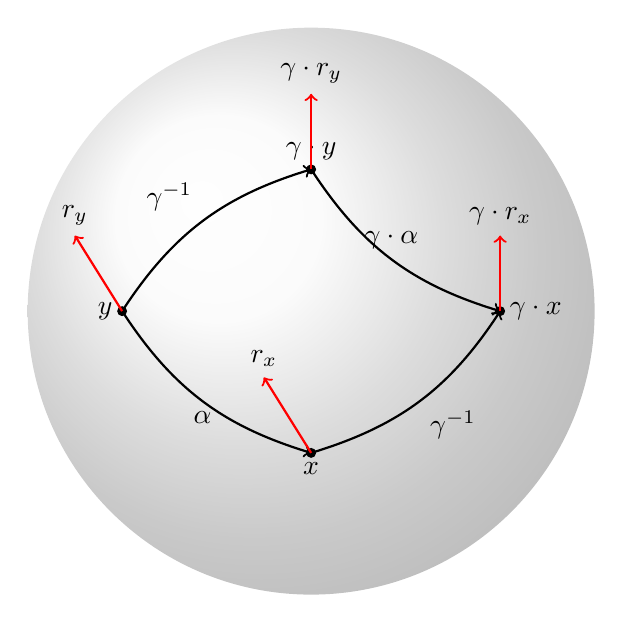
\begin{tikzpicture}[scale=1.2]
    % 背景球体效果
    \shade[ball color=gray!10, opacity=0.4] (0,0) circle (3cm);
    
    % 定义坐标
    \coordinate (X) at (0, -1.5);
    \coordinate (Y) at (-2, 0);
    \coordinate (gX) at (2, 0);
    \coordinate (gY) at (0, 1.5);
    
    % 画点
    \fill (X) circle (1.5pt) node[below] {$x$};
    \fill (Y) circle (1.5pt) node[left] {$y$};
    \fill (gX) circle (1.5pt) node[right] {$\gamma \cdot x$};
    \fill (gY) circle (1.5pt) node[above] {$\gamma \cdot y$};
    
    % 画路径
    \draw[thick, ->] (Y) to[bend right=20] node[below] {$\alpha$} (X);
    \draw[thick, ->] (gY) to[bend right=20] node[above] {$\gamma \cdot \alpha$} (gX);
    \draw[thick, ->] (Y) to[bend left=20] node[above left] {$\gamma^{-1}$} (gY);
    \draw[thick, ->] (X) to[bend right=20] node[below right] {$\gamma^{-1}$} (gX);
    
    % 画标架向量 (红色箭头)
    \draw[thick, red, ->] (Y) -- ++(-0.5, 0.8) node[black, above] {$r_y$};
    \draw[thick, red, ->] (X) -- ++(-0.5, 0.8) node[black, above] {$r_x$};
    \draw[thick, red, ->] (gY) -- ++(0, 0.8) node[black, above] {$\gamma \cdot r_y$};
    \draw[thick, red, ->] (gX) -- ++(0, 0.8) node[black, above] {$\gamma \cdot r_x$};
\end{tikzpicture}
\end{center}

现在设 $r_y$ 是 $R_H$ 在另一点 $y$ 处的标架。如上图所示，我们可以选取一条从 $y$ 到 $x$ 的路径 $\alpha$。我们将 $r_y$ 沿 $\alpha$ 平行移动得到 $x$ 处的标架 $r_x$。
由于 $r_y$ 和 $\gamma \cdot r_y$ 来自底流形 $X$ 上同一点的同一个标架，对于 $r_x$ 和 $\gamma \cdot r_x$ 也同理；且由于 $\alpha$ 和 $\gamma \cdot \alpha$ 来自 $X$ 上同一条路径，我们知道 $\gamma \cdot r_x$ 来自于 $\gamma \cdot r_y$ 沿 $\gamma \cdot \alpha$ 的平行移动。
这意味着 $\varphi(\gamma \cdot r_x) = \varphi(\gamma \cdot r_y)$ 且 $\varphi(r_x) = \varphi(r_y)$。因此 $g_\gamma(r_y) = g_\gamma(r_x)$。
\end{proof}

\begin{proposition}\label{periodinvariant}
周期映射在表示 $\rho$ 下是等变的，即 $\mathcal{P}(\gamma \cdot x) = \rho(\gamma) \cdot \mathcal{P}(x)$。
\end{proposition}

\begin{proof}
\[ \mathcal{P}(\gamma \cdot x) = \varphi_{P_H}(\gamma \cdot x) = \varphi(\gamma \cdot P_H(x)) = \rho(\gamma) \cdot \varphi(P_H(x)) = \rho(\gamma) \cdot \mathcal{P}(x) \]
\end{proof}

\subsection{Hodge表示与稳定性}

设 $V = \oplus_{p+q=k} V^{p,q}$ 为具有极化Hodge结构的复向量空间。

\begin{definition}
极化Hodge表示 $\Pi: G_0 \to \text{GL}(V)$ 是一个复表示，使得 $K_0$ 的作用保持Hodge分解，且 $\g$ 的作用与Hodge类型兼容（即 $\g^{k, -k} \cdot V^{p,q} \subset V^{p+k, q-k}$），并且半线性形式 $s$ 被 $G_0$ 保持。
\end{definition}

特别地，伴随表示 $\Ad: G_0 \to \text{GL}(\g)$ 是极化Hodge表示。

\begin{definition}
假设 $X$ 是紧致的，一个Hodge丛主系统 $(P, \theta)$ 称为 $\Pi$-稳定的，如果Hodge丛系统 $P \times_K V$ 是稳定的。
\end{definition}

对于非紧情况，我们需要选择度量 $P_H$ 使得 $\Lambda F_{\nabla^{hs}}$ 有界。

\begin{lemma}
设 $\Pi: G_0 \to V$ 为极化Hodge表示，如果 $\Lambda F_{\nabla^{hs}}$ 有界，则 $\Lambda {}^V F_{\nabla^{hs}}$ 也有界。
\end{lemma}

\begin{definition}
假设 $X$ 非紧，令 $(P, \theta, P_H)$ 为带有度量 $P_H$ 的Hodge丛主系统，满足 $\Lambda F_{\nabla^{hs}}$ 有界。我们称 $(P, \theta, P_H)$ 是 $(\Pi, P_H)$-稳定的，如果Hodge丛系统 $P \times_K V$ 关于度量 $(P_H, H)$ 是解析稳定的。
\end{definition}

\subsection{主 VHS 的构造}

我们有如下由 Simpson 得到的结果。

\begin{theorem}\label{prop8.1}
如果 $(P, \theta, P_H)$ 关于某个不可约极化Hodge表示族 $\{\Pi_i\}_i$ 是 $(\Pi_i, P_H)$-稳定的，且该表示族忠实地表示了 $\g$，即 $\oplus_i d\Pi_i$ 是单射，那么存在一个度量 $P_K$ 使得 $\Lambda F_{\nabla^{hs}} = 0$。如果此外 $X$ 是紧致的且 $c_2(P \times_K \g) \cdot [\omega]^{n-2} = 0$，则 $F_{\nabla^{hs}} = 0$，因此这给出了一个主Hodge结构形变。
\end{theorem}

\begin{proof}
固定一个初始度量 $P_{H_0}$ 使得解析稳定性的概念是良定义的。如果 $\Pi$ 是上述 $G_0$ 到 $(V, H) = (\oplus V_i, \oplus H_i)$ 的表示，那么 $H$ 和 $P_{H_0}$ 共同给出了 $P \times_K V = \mathcal{V} = \oplus \mathcal{V}_i$ 上的一个度量 $H_0$，这是一个 Hodge 丛系统的直和，或者说是具有 $U(1) \times U(1)$ 对称性的 Higgs 丛。此时我们可以调用定理~\ref{th1} 来运行 H-Y-M 流：
\[ h^{-1}\dot{h} = -\sqrt{-1}\Lambda F_{\nabla^{hs}_{H(t)}} \]
其中 $H(t) = H_0h$。由于曲率保持 $U(1) \times U(1)$ 对称性且解是唯一的，$h(t)$ 也保持该作用，特别是 $h$ 保持Hodge分解。稳定性条件给出了一个极限 $h_\infty$。为了证明 $h_\infty$ 来自于一个度量 $P_K$，只需证明对任意 $x$，有 $h_\infty(x) \in \Pi(K)$。为此，我们需要用到 Tannakian 范畴理论中的以下定理。

\begin{theorem}[Chevalley]
$GL(V)$ 的任意代数子群 $G$ 均可作为由 $V$ 的张量积、直和及对偶构成的向量空间 $T(V)$ 中一维子空间的稳定子出现。
\end{theorem}

或者等价地，我们可以将 $G$ 刻画为由 $V$ 和 $V^*$ 中的元素组成的有限个张量的稳定子。在我们的情形下，$\Pi(G)$ 由一组张量刻画。因此只需证明给定这样一个张量 $w$，有 $h(t) \cdot w = w$。由于 $w$ 是 $\Pi(G)$ 不变的，故 $\g \cdot w = 0$。

假设 $w \in T(V) \otimes T(V^*)$，令 $\mathcal{W}$ 为关联于由 $w$ 张成的线性子空间的线丛，$\mathcal{T}$ 为关联于 $T(V) \otimes T(V^*)$ 的丛，且 $\otimes h$ 为 $\mathcal{T}$ 上热方程的解。由于 $\Lambda F_0$ 是 $\g$-值的，故 $\Lambda F_0 \cdot w = 0$。于是由热方程解的唯一性可知 $\otimes h|_{\mathcal{W}} = \id$。另一方面，热方程的解与张量及对偶表示是兼容的，我们有 $h \cdot w = \otimes h \cdot w = w$。从而我们证明了 $h \in \Pi(G)$。

但我们知道 $h$ 保持Hodge分解，于是 $\Ad(h)\g^{p,-p} = \g^{p,-p}$（由于表示在李代数层面上是忠实的，我们将 $\g$ 的像与 $\g$ 等同）。由于 $K$ 根据定义是稳定Hodge结构的极大子群，我们有 $h \in \Pi(K)$，因此 $H_\infty$ 来自于 $K$-丛 $P$ 的一个 $K_0$-约化 $P_{H_\infty}$。稳定性条件表明 $\Lambda F_{\nabla^{hs}_{H_\infty}} = 0$，由于表示在李代数层面上是忠实的，我们在主丛上有 $\Lambda F_{\nabla^{hs}} = 0$。

如果 $X$ 紧致且 $c_2(P \times_K \g) \cdot [\omega]^{n-2} = 0$，则 $c_2(P \times_K V) \cdot [\omega]^{n-2} = 0$。事实上，由于 $\g$ 半单，$\g$ 上由 Ad-不变双线性对称形式张成的线性空间是一维的，因此 $c_2(P \times_K V) = C \cdot c_2(P \times_K \g)$，其中 $C$ 为常数。然后我们可以应用命题~\ref{prop3.3} 来证明 $F_{\nabla^{hs}} = 0$。
\end{proof}
\subsection{一个例子}

令 $V = \oplus V^{p,q}$ 为具有不定 Hermitian 形式 $s$ 的极化Hodge结构。定义 $G_0 := \Au(V, s)/U(1)$，则 $K_0 = \Au(V, h)/U(1)$。$G_0$ 是单李群，复化李代数 $\g = \En(V)^\perp$。$G_0$ 是极化Hodge群。

\begin{definition}
以 $V$ 为模型的射影 VHS 是一个主 VHS $(P_H, \nabla^{hs})$。
\end{definition}

\begin{lemma}\label{lemmabundletovhs}
假设 $X$ 紧致。如果Hodge丛系统 $E = \oplus E^{p,q}$ 是具有相同斜率的稳定丛的直和，并满足命题~\ref{prop3.3} 中的等式，则它诱导一个主 VHS。周期映射的微分是 $\theta: T(\tilde{X}) \to \En(E)^{-1, 1}$。
\end{lemma}
\begin{proof}
固定一个纤维，记为 $V$。来自 $E^{p,q}$ 的全纯标架模掉等价关系 $e \sim z \cdot e$ 给出了一个 $K$-torsor，即一个全纯主 $K$-丛，其中 $K = (\En(V)^\perp)^{0,0}$。Higgs 场给出了一个 $\En(V)^{-1,1}$-值的张量形式 $\theta$。
由于 $E$ 是多重稳定的（poly-stable），我们可以运行 H-Y-M 流并利用定理~\ref{th1} 和命题~\ref{prop3.3} 在 $E$ 上得到一个度量 $H$，使得 $F^\perp_{\nabla^{hs}_H} = 0$。
于是，射影酉标架给出了一个具有零曲率的 $K_0$-torsor（即一个度量）。
\end{proof}

\begin{corollary}\label{examplecor}
假设 $\mathcal{L}$ 是Hodge流形 $X$（带极化 $\Theta$）上的线丛，且存在非零态射 $\psi: \mathcal{L} \to \Omega_X^1$。如果 $\mathcal{L} \cdot \Theta^{n-1} > 0$，则 $\mathcal{L} \cdot \Theta^{n-2} \le 0$；若此外等号成立，则存在非平凡表示 $\pi_1(X) \to \text{PSL}(2, \mathbb{R})$ 以及从 $\tilde{X}$ 到上半平面的等变映射。
\end{corollary}

\begin{proof}
考虑丛 $\mathcal{L} \oplus \mathcal{O}_X$，将 $\mathcal{O}_X$ 视为 $(0, 1)$ 分量，$\mathcal{L}$ 视为 $(1, 0)$ 分量。定义 Higgs 场 $\theta = \begin{pmatrix} 0 & 0 \\ \psi & 0 \end{pmatrix}$。这是一个稳定的Hodge丛系统。利用命题~\ref{prop3.3}和上述引理，当等号成立时，得到 $G_0 = \text{PSU}(1, 1)$ 和 $K_0 \cong U(1)$ 的射影 VHS。齐性空间 $G_0/K_0 \cong \mathbb{H}$（上半平面）。
\end{proof}
\subsection{单值化 (Uniformization)}

\subsubsection*{Hermitian 对称空间}

\begin{definition}
Hermitian 类型的Hodge群是指类型为 $\mathfrak{g} = \mathfrak{g}^{0,0} \oplus \mathfrak{g}^{-1,1} \oplus \mathfrak{g}^{1,1}$ 且没有紧致因子的Hodge群。对于这样的群，$K_0$ 成为极大紧子群。齐性空间 $G_0/K_0$ 是非紧类型的 Hermitian 对称空间。
\end{definition}

实际上，以下三个概念是等价的：
\begin{center}
\begin{tikzpicture}[>=stealth, node distance=2cm, auto]
    % 定义节点
    \node (A) at (0, 2) {$G_0/K_0$};
    \node (B) at (-3, 0) {有界对称域};
    \node (C) at (3, 0) {Hermitian 对称空间};
    
    % 定义连线箭头
    \draw[<->] (A) -- (B);
    \draw[<->] (A) -- (C);
    \draw[<->] (B) -- (C);
\end{tikzpicture}
\end{center}

\begin{definition}
$X$ 的单值化丛是一个Hodge丛主系统 $(P, \theta)$，使得
\[ \theta: T(X) \to P \times_K \mathfrak{g}^{-1,1} \]
是同构。
\end{definition}

值得注意的是，如果 $G_0$ 没有中心，则 $\Ad$ 是忠实的，那么该数据等价于 $T(X)$ 的结构群从 $\mathrm{GL}(n, \mathbb{C})$ 约化到 $K$，这里我们将 $K$ 与其伴随表示 $\Ad: K \to \mathrm{GL}(\mathfrak{g}^{-1,1})$ 的像等同，并将 $\mathrm{GL}(\mathfrak{g}^{-1,1})$ 与 $\mathrm{GL}(n, \mathbb{C})$ 等同。更确切地说，如果我们能指定 $T(X)$ 的一些标架，使得它们逐点构成一个 $K'$-torsor，其中 $K' = \Ad(K)$（对于某个无中心的 $G_0$ 的 $K$），并且 $K'$ 在标架上的右作用与 $K$ 在 $\mathfrak{g}^{-1,1}$ 上的伴随作用相同，那么我们可以从这些数据得到一个单值化丛。实际上，记标架丛为 $P$，如果我们通过 $\Ad$ 将 $K'$ 与 $K$ 等同，那么 $P$ 就是一个 $K$-丛，显然有
\[ T(X) \cong P \times_{\text{st}(K')} \mathfrak{g}^{-1,1} \cong P \times_K \mathfrak{g}^{-1,1}. \]

\begin{example}
假设 $T(X) = \oplus_{i=1}^n L_i$，其中 $L_i$ 为线丛。那么我们可以考虑保持该分解的标架，此时标架丛 $P$ 是一个 $K' = \mathbb{C}^{*n}$-丛。实际上，$K'$ 来自于与 Hermitian 类型Hodge群 $G_0 = \mathrm{PSU}(1,1)^n$ 关联的 $K$ 的伴随表示，其关联的有界对称域为 $\mathbb{D}^n$。
\end{example}

让我们详细讨论一下。令 $G_0 = \mathrm{PSU}(1,1)$。它看起来像
\[ \begin{pmatrix} \alpha & \beta \\ \bar{\beta} & \bar{\alpha} \end{pmatrix}, \quad |\alpha|^2 - |\beta|^2 = 1 \]
其李代数 $\mathfrak{su}(1,1)$ 有三个生成元
\[ \mathfrak{k}_0 = \begin{pmatrix} i & 0 \\ 0 & -i \end{pmatrix}, \quad \mathfrak{p}_1 = \begin{pmatrix} 0 & 1 \\ 1 & 0 \end{pmatrix}, \quad \mathfrak{p}_2 = \begin{pmatrix} 0 & i \\ -i & 0 \end{pmatrix} \]
其复化 $\mathfrak{g}$ 有三个生成元
\[ \mathfrak{g}^{0,0} = \begin{pmatrix} 1 & 0 \\ 0 & -1 \end{pmatrix} \]
\[ \mathfrak{g}^{-1,1} = \frac{1}{2}(\mathfrak{p}_1 - i\mathfrak{p}_2) = \begin{pmatrix} 0 & 1 \\ 0 & 0 \end{pmatrix}, \quad \mathfrak{g}^{1,-1} = \frac{1}{2}(\mathfrak{p}_1 + i\mathfrak{p}_2) = \begin{pmatrix} 0 & 0 \\ 1 & 0 \end{pmatrix} \]
并且
\[ K = \begin{pmatrix} z & 0 \\ 0 & z^{-1} \end{pmatrix} / \{\pm \id\} \cong \mathbb{C}^* / \{\pm \id\} \]
$K$ 在 $\mathfrak{g}^{-1,1}$ 上的伴随表示是乘以 $z^2$。因此表示 $K'$ 的像仍然是 $\mathbb{C}^*$。

\begin{example}[典范 Higgs 丛]
设 $X$ 是紧致的，丛 $\Omega_X^1 \oplus \mathcal{O}_X$ 连同 $\theta = T(X) \cong \mathrm{Hom}(\Omega_X^1, \mathcal{O}_X)$ 被称为典范 Higgs 丛。如果它容许一个度量使得 $F_{\nabla^{ns}}^\perp = 0$，那么它是一个 $G_0 = \mathrm{PU}(n,1)$ 的单值化形变。
\end{example}

这直接由引理~\ref{lemmabundletovhs}得出。$\mathrm{PU}(n,1)$ 是 Hermitian 类型的Hodge群，其关联的有界对称域是单位球 $\mathbb{B}^n$。其Hodge类型如下：
\[ \mathfrak{g}^{0,0} = \left\{ \begin{pmatrix} A & 0 \\ 0 & -\mathrm{tr}(A) \end{pmatrix} \middle| A \in M_n(\mathbb{C}) \right\} \]
\[ \mathfrak{g}^{-1,1} = \left\{ \begin{pmatrix} 0 & v \\ 0 & 0 \end{pmatrix} \middle| v \in \mathbb{C}^n \right\} \quad \mathfrak{g}^{1,-1} = \left\{ \begin{pmatrix} 0 & 0 \\ w & 0 \end{pmatrix} \middle| w \in (\mathbb{C}^n)^T \right\}. \]

\subsubsection*{单值化 VHS}

单值化Hodge结构形变是带有一个平坦度量 $P_H$ 的单值化丛 $(P, \theta)$。

\begin{proposition}
设 $X$ 是完备 Kähler 流形，$\tilde{X}$ 为其万有覆叠。则 $\tilde{X}$ 同构于有界对称域 $\mathcal{D}$ 当且仅当存在一个关于某个满足 $\mathcal{D} = G_0/K_0$ 的Hodge群 $G_0$ 的单值化 VHS，且 $\theta^{-1}$ 有界。
\end{proposition}

\begin{proof}
假设存在这样的单值化形变。由于 $\theta$ 是周期映射 $\mathcal{P}$ 的微分，它是一个局部微分同胚。因为它是 $\pi_1(X)$-等变的，我们可以证明 $\mathcal{P}$ 是闭映射，因此是满射。由于 $dP^{-1} = \theta^{-1}$ 有界且 $\tilde{X}$ 完备，易证 $\mathcal{P}$ 是覆叠映射。但由于 $\mathbb{D}$ 是单连通的，故 $\mathcal{P}$ 是同构。

反之，如果 $\tilde{X} \cong \mathbb{D}$ 且它是 $\pi_1(X)$ 等变的。令 $G_0$ 为 $\mathbb{D}$ 的全纯自同构群，则 $\mathbb{D} \cong G_0/K_0$，$\pi_1(X)$ 通过全纯自同构作用于 $\mathbb{D}$，因此我们得到了一个表示。只需在 $\mathbb{D}$ 上构造一个主 VHS，它是自然产生的。我们将 $G_0$ 视为 $\mathbb{D}$ 上的主 $K_0$-丛，根据 Cartan 分解，其 Cartan-Maurer 形式 $\omega = g^{-1}dg$ 分解为 $\omega_{\mathfrak{k}}$ 和 $\omega_{\mathfrak{h}}$，前者是联络形式，后者是张量形式。我们有 $d\omega + \frac{1}{2}[\omega, \omega] = 0$。将 $G_0$ 的结构群扩张到 $K$，得到 $P = G_0 \times_{K_0} K$。$\omega_{\mathfrak{h}}$ 分裂为 $\omega_{\mathfrak{h}^-}$ 和 $\omega_{\mathfrak{h}^+}$。由于曲率 $\Omega_{\mathfrak{k}} = d\omega_{\mathfrak{k}} + \frac{1}{2}[\omega_{\mathfrak{k}}, \omega_{\mathfrak{k}}] = -\frac{1}{2}[\omega_{\mathfrak{h}}, \omega_{\mathfrak{h}}]$，这意味着曲率的 $(0,2)$ 部分消失，因此 $\omega_{\mathfrak{k}}$ 的 $(0,1)$ 部分给出了 $P$ 上的全纯结构，$\omega_{\mathfrak{h}^-}$ 是一个 Higgs 场。如果我们进一步将这些结构扩张到 $R_H = G_0 \times_{K_0} G_0$，那么 $\omega$ 就是我们想要的平坦 Hitchin-Simpson 联络。

我们甚至可以检查周期映射是什么！实际上，很容易看出 $[g, g^{-1}]$ 是关于 $\omega$ 的平坦截面，因此周期映射是恒等映射 $\id$。
\end{proof}

\subsubsection*{单值化丛的稳定性}

将 $\mathfrak{g}$ 分解为单理想 $\mathfrak{g} = \oplus \mathfrak{g}_i$。它们是子Hodge结构，如果 $G_0$ 是连通的，它们是 $G_0$ 的Hodge表示。为了更一般化，我们不假设连通性。如果 $(P, \theta)$ 是单值化丛，局部上我们可以将 $P \times_K \mathfrak{g}$ 分解为 $\oplus \mathfrak{g}_i$，但全局上它们被 $G$ 的伴随表示扭曲。然而，我们可以找到 $P \times_K \mathfrak{g}$ 的唯一最细全局分解 $\oplus U_j$，使得 $U_j$ 局部上是 $\{\mathfrak{g}_i\}_i$ 的固定子集的直和，即单李代数集合分解为不相交的子集 $\mathfrak{u}_j$。$U_j$ 可能不来自 $G$ 的表示，但我们可以找到 $G$ 的子群 $G'$ 使得 $P$ 的结构群可以约化为 $K' = K \cap G'$，且 $U_j = P' \times_{K'} \mathfrak{u}_j$，同时整个伴随丛的全纯结构被保持，即 $P \times_K \mathfrak{g} \cong P' \times_{K'} \mathfrak{g}$。如果需要，我们将始终假设已进行此类约化。

\begin{definition}
一个单值化丛是稳定的，如果它对所有 $j$ 都是 $\mathfrak{u}_j$-稳定的。
\end{definition}

调用一个关于李代数的引理。

\begin{lemma}
假设 $\mathfrak{g}_0$ 是我们考虑类型的单李代数。如果 $e \in \mathfrak{g}^{-1,1}$，则
\[ [\mathfrak{g}^{-1,1}, [\mathfrak{g}^{-1,1}, e]] = \mathfrak{g}^{-1,1}. \]
\end{lemma}

\begin{corollary}
假设 $\mathfrak{g}$ 是半单的。如果 $W \subset \mathfrak{g}$ 是一个子Hodge结构使得 $[\mathfrak{g}^{-1,1}, W] \subset W$，则 $\dim W^{-1,1} \ge \dim W^{1,-1}$。如果等号成立，则 $W$ 是 $\mathfrak{g}$ 的理想的直和。
\end{corollary}

\begin{corollary}
假设 $(P, \theta)$ 是单值化Hodge丛系统。则以下条件等价：
\begin{enumerate}
    \item $(P, \theta)$ 是稳定的。
    \item $P \times_K \mathfrak{g}$ 是度数为零的稳定系统的直和。
    \item $P \times_K \mathfrak{g}$ 的每个满足 $\deg(W) \ge 0$ 的饱和Hodge层子系统 $W$ 局部上是某些 $\mathfrak{g}_i$ 的直和。
\end{enumerate}
\end{corollary}

\begin{proof}
1. $\Rightarrow$ 2. 写出 $P \times_K \mathfrak{g} = U_j$，则 $U_j$ 是稳定的，且由于 $\mathfrak{u}_j$ 是半单的，它的度数为零。
2. $\Rightarrow$ 3. 由于 $P \times_K \mathfrak{g}$ 是多重稳定的 (polystable)，$\deg W = 0$ 且 $P \times_K \mathfrak{g} = W \oplus W'$。特别地，$W'$ 也是Hodge丛系统。对 $W$ 和 $W'$ 应用上一个推论，两者均等号成立。
3. $\Rightarrow$ 1. 如果 $W \subset U_j$ 是满足 $\deg W \ge 0$ 的饱和Hodge层子系统，则 $W$ 局部上是某些 $\mathfrak{g}_i$ 的直和，因为 $U_j$ 是最细的，所以 $W = U_j$。
\end{proof}

\begin{theorem}
假设 $X$ 是紧致的。$\tilde{X} \cong \mathbb{D}$ 当且仅当存在一个结构群 $G_0$ 对应于 $\mathbb{D}$ 的单值化丛 $(P, \theta)$，使得 $(P, \theta)$ 是稳定的且 $c_2(P \times_K \mathfrak{g}) \cdot [\omega]^{n-2} = 0$。
\end{theorem}

\begin{proof}
每个 $U_j$ 来自 $G'$ 到 $\mathfrak{u}_j$ 的不可约Hodge表示。应用定理 9 我们知道 $(P, \theta)$ 是单值化 VHS。应用命题 13 我们知道 $\tilde{X} \cong \mathbb{D}$。反之，应用命题 13 我们得到单值化 VHS $(P, \theta)$。因此 $P \times_K \mathfrak{g}$ 的所有陈类消失，且它是多重稳定的。应用上述推论，我们知道 $(P, \theta)$ 是稳定的。
\end{proof}

\begin{corollary}
设 $\mathbb{D}$ 如前所述，设 $X$ 是光滑射影簇。则对于任意 $\sigma \in \Au(\mathbb{C}/\mathbb{Q})$，如果 $X$ 被 $\mathbb{D}$ 单值化，那么 $X^\sigma$ 也是。
\end{corollary}

\begin{proposition}
假设 $X$ 是紧致的且 $(P, \theta)$ 是单值化丛。则
\[ \theta: T(X) \cong P \times_K \mathfrak{g}^{-1,1} \cong \oplus_j V_j. \]
如果 $V_j$ 是半稳定的且度数严格小于零，则 $(P, \theta)$ 是稳定的。因此如果 $c_2(P \times_K \mathfrak{g}) \cdot [\omega]^{n-2} = 0$，则 $(P, \theta)$ 是 $X$ 的单值化 VHS。
\end{proposition}

\begin{proof}
假设 $G$ 是连通的。则 $K$ 在 $\mathfrak{g}_i^{-1,1}$ 上的作用是不可约的，因此 $V_i = P \times_K \mathfrak{g}_i^{-1,1}$。$P \times_K \mathfrak{g}_i^{-1,1}$ 和它们的对偶 $P \times_K \mathfrak{g}_i^{1,-1}$ 是半稳定的。李括号
\[ [\cdot, \cdot]: P \times_K \mathfrak{g}_i^{-1,1} \otimes P \times_K \mathfrak{g}_i^{1,-1} \to P \times_K \mathfrak{g}_i^{0,0} \]
是满射，因此右边是度数为零的半稳定的。假设 $W \subset P \times_K \mathfrak{g}_i$ 是Hodge层子系统。则 $\deg(W^{0,0}) \le 0$ 且 $\deg(W^{1,-1}) \le -\mathrm{rank}(W^{1,-1}) \cdot \mu$ 以及 $\deg(W^{-1,1}) \le \mathrm{rank}(W^{1,1}) \cdot \mu$，其中 $\mu(V_i) < 0$ 是斜率。因此
\[ \mu(W) \le (\mathrm{rank}(W^{-1,1}) - \mathrm{rank}(W^{1,-1})) \cdot \mu(V_i) \le 0 \]
如果等号成立，则利用推论 15 可知 $W=V_i$，因此 $V_i$ 是稳定的。

假设 $G$ 不连通。令 $G^o$ 为 $G$ 的连通分支，$K^o$ 为 $K$ 的连通分支。则 $P/K^o$ 是一个 $K/K^o$-主丛，它也是 $X$ 的覆叠空间。我们有单值性 (monodromy) $\pi_1(X) \to K/K^o$。找一个覆叠 $\pi: X^o \to X$，其基本群是单值性的核，那么我们可以在 $X^o$ 上将 $P$ 的结构群从 $K$ 约化到 $K^o$。拉回 $\pi^*(V_j)$ 是半稳定的。如果我们关于 $K^o$ 作用分解 $TX^o = \oplus V_k^o$，则 $\pi^*(V_j)$ 是某些 $V_k^o$ 的直和。因此每个 $V_k^o$ 都是负度数半稳定的。根据上述关于连通 $G^o$ 的讨论，它们是稳定的，因此 $P \times_K \mathfrak{g} = P^o \times_{K^o} \mathfrak{g}$ 在 $X^o$ 上是多重稳定的。如果 $W$ 是 $X$ 上满足 $\deg(W) \ge 0$ 的Hodge层子系统，那么它的拉回 $\pi^*W$ 具有零度数，必定是 $P^o \times_{K^o} \mathfrak{g}$ 的稳定子丛的直和。因此由推论 15，它是单理想的局部直和，对于 $W$ 也是如此，因此由推论 16，$(P, \theta)$ 是稳定的。
\end{proof}

\begin{corollary}
假设 $X$ 是紧致的。如果 $T_X = \oplus_{i=1}^n L_i$ 是负度数线丛的直和，并且 $(c_1(X)^2 - 2c_2(X)) \cdot [\omega]^{n-2} = 0$，则 $X$ 被 $\mathbb{B}^n$ 单值化。
\end{corollary}

\begin{proof}
由例 1 的讨论可知，我们有一个 $K = (\mathbb{C}^*/\{\id, -\id\})^n$ 的单值化丛。其关联的有界对称域是 $\mathbb{B}^n$。直接计算表明 $c_2(P \times_K \mathfrak{g}) = 2c_2(X) - c_1(X)^2$。
\end{proof}

接下来调用例 2 中的典范 Higgs 丛 $W$。

\begin{proposition}[Miyaoka-Yau 不等式]
假设 $X$ 是紧致的。如果 $W$ 是稳定的，则
\[ \left( 2c_2(X) - \frac{n}{n+1} c_1(X)^2 \right) \cdot [\omega]^{n-2} \ge 0 \]
如果等号成立，则 $X$ 被 $\mathbb{B}^n$ 单值化。
\end{proposition}

如果 $X$ 是紧致曲线，则陈类条件平凡成立，$W$ 稳定当且仅当 $X$ 的亏格 $g$ 大于 2。因此，如果 $g \ge 2$，$X$ 被 $\mathbb{B}$ 单值化，这就是经典的单值化。

\begin{proposition}
假设 $X$ 是紧致 Kähler 曲面。如果 $c_1(X)^2 \ge 3c_2(X)$，$c_1(X)^2 \ge 0$ 且 $c_1(X) \cdot [\omega] < 0$，则 $W$ 是稳定的，从而 $c_1(X)^2 = 3c_2(X)$ 且 $\tilde{X} = \mathbb{B}^2$。
\end{proposition}

\begin{proof}
只需证明对偶 Higgs 丛 $W^* = (\mathcal{O}_X, T_X)$ 是稳定的。秩为 2 的唯一饱和子层是 $T_X$，由 $c_1(X) \cdot [\omega] < 0$ 满足条件。秩为 1 的饱和子层是 $T_X$ 的可逆子层，它们在有限集之外是线子丛。设 $L$ 为这样的子层。我们必须证明 $c_1(L) \cdot [\omega] < \frac{1}{3} c_1(X) \cdot [\omega]$。反之假设不成立。令 $M = T_X/L$，它是余维数 1 的线丛。令 $N = M^{**}$，则它是线丛，且 $M \hookrightarrow N$ 的商支集在有限集上。$(\mathcal{O}_X, N)$ 是一个Hodge丛系统，且
\[ c_1(N) \cdot [\omega] \le \frac{2}{3} c_1(X) \cdot [\omega] \le 0 \]
因此它是稳定的。B-G 不等式蕴含 $c_1(N)^2 \le 0$。在 Grothendieck 群中 $T_X$ 等于 $N + L - (N/M)$，因此
\[ \begin{aligned} c_2(X) &= c_1(N)c_1(L) - c_2(N/M) \\ &= c_1(X)c_1(N) - c_1(N)^2 - c_2(N/M) \\ &\ge c_1(N)c_1(X) - c_1(N) \end{aligned} \]
最后一个不等式成立是因为 $c_2(N/M)$ 等于其支集中点的非正和。因此
\[ (c_1(N) - 2c_1(X))^2 \ge 4(c_1(X)^2 - 3c_2(X)) \ge 0 \]
由我们的假设。另一方面，我们将Hodge指数定理应用于 $H^{1,1}(X, \mathbb{R})$。其上的相交形式具有符号 $(1, h^{1,1}-1)$，我们可以选择由 $\omega$ 张成的正定子空间。因此 $c_2(X)$ 位于正锥的负半部的内部，而 $3c_1(N)$ 在 $2c_1(X)$ 下方的锥外。因此 $3c_1(N) - 2c_1(X)$ 严格在锥外，所以它的平方严格为负，导致矛盾。
\end{proof}
\subsection{非紧曲线上的Hodge丛}
令$X$为一个非紧黎曼面，$\overline{X}$为$X$的一个光滑紧化，令$\omega$为$\overline{X}$上的一个 K\"ahler 形式，其在$X$上的限制依然记为$\omega$。令$j:X\to \overline{X}$为其嵌入映射，令$Y=\overline{X}-X$. 
\begin{definition}\label{regularsytemofhodgebundle}
    一个$X^{alg}$上的\textbf{正则Hodge丛}是一个代数Hodge丛$E$并存在以下尊重Hodge分解的滤链：
    \[
    j_*^{alg}E=\bigcup_{\alpha\in \R^{Y}} E_{\alpha}
    \]
其中$E_\alpha$皆为凝聚子层，我们赋予$\R^{Y}$自然的偏序结构，我们要求该滤链关于偏序结构是左连续并且递降的。并且我们要求Higgs场满足
\[
\theta: E^{p,q}_\alpha \to E^{p-1,p+1}_\alpha\otimes \Omega_X^1\langle\log(Y)\rangle
\]
\end{definition}
下面我们会看到这样的定义是自然的。假设我们有一个全纯的Hodge丛$E\to X$，如果$E$上存在一个在奇点附近行为较好的和Hodge结构相容的度量$h$ （我们总是假设度量和Hodge结构相容），我们可以通过如下方式构造出一族子层$a_hE^{p,q}=\bigcup_{\alpha\in \R^{Y}} E^{p,q}_\alpha$：我们定义$E^{p,q}_\alpha$为$j^{an}_*E^{p,q}$当中满足以下条件的子层，对任意的$y\in Y$，假设$y\in\U$，我们只选取增长速度满足
\[
|s|_h\leq C r^{\alpha_y-\epsilon},\quad \text{对充分小的}\epsilon>0
\]
的那些截面$s$。

Simpson\cite{Si1}证明了以下定理，
\begin{theorem}
    假设$(E,\overline{\partial},\theta, h)$是一个带度量的Hodge丛，并且度量$h$满足
    \[
    \int_X |F_{\nabla^{hs}_h}|^p <\infty,\quad p>1
    \]
    则如上定义的$E_\alpha$是凝聚层，并且$\theta$满足
    \[
    \theta: E^{p,q}_\alpha \to E^{p+1,q-1}_\alpha \otimes \Omega_X^1\langle\log Y\rangle
    \]
    因此$E$是一个正则Hodge丛。上述的构造 $a$ 和取行列式，对偶，张量积可交换。如果$h$和$h'$两个度量满足$a_h=a_h'$，那$h$和$h'$是可比的。并且我们有$a$作为从带$L^p$--曲率度量的Hodge丛打到正则Hodge丛的函子，它是一个范畴等价。
\end{theorem}

我们先证明以下引理：

\begin{lemma}\label{boundofHiggs}
    对于Hodge丛$(E,\overline{\partial},\theta)$，固定某个$p>1$。对任意的度量$h$满足
    \[
    \int_X |F_{\nabla^{hs}_{h}}|^p<\infty,
    \]
    则Higgs场满足
    \[
    \sup |\theta|\leq \frac{C}{|z\log|z||}
    \]
    这里$z$是某个$y\in Y$附近的一个小坐标邻域，常数$C$被曲率的$L^p$--范数所决定。
\end{lemma}
\begin{proof}
   不妨给坐标邻域赋予标准欧式度量。因此张量丛$(\En(E))^{-1,1}\otimes \Omega_X^1$的Chern曲率完全由$\nabla_h^2$的伴随作用给出，其中$\nabla_h$是丛$(E,\overline{\partial},h)$的Chern曲率张量。由于全纯子丛的曲率小于等于整体曲率的限制，因此如果我们把$\theta$看成$(\En(E))^{-1,1}\otimes \Omega_X^1$的一个线丛子丛的话，在$\theta$不为0处，我们有以下不等式
   \[
   \Delta \log|\theta|^2\leq \frac{\langle2i\ad\Lambda\nabla_h^2(\theta),\theta \rangle_h}{|\theta|^2}.
   \]

   令一方面，任给切向量$v\in T^{1,0}$，$\theta(v)$是周期域$G_0/K_0$的切向量，由\cite{griffiths1969locally}中的结论，周期域的全纯截面曲率在$\g^{-1,1}$方向上是严格负的，因此我们有
\[
\frac{R(\theta(v),\overline{\theta}(\bar{v}),\theta(v),\overline{\theta}(\bar{v}))}{|\theta(v)|^4}=-\langle [[\theta(v),\overline{\theta}(\bar{v})],\theta(v)],\theta(v)\rangle\leq -C
\]
取局部坐标$z$使得$\omega=\frac{i}{2}\diff z\wedge \diff \overline{z}$以及丛的酉标架。在此平凡化下
\[\theta=\phi\diff z, \quad \overline{\theta}=\phi^\dagger \diff \overline{z}\]
\[|\theta|^2=2\tr(\phi\phi^\dagger),\quad [\theta,\theta^\dagger]=(\phi\phi^\dagger-\phi^\dagger\phi)\diff z\wedge \diff \overline{z}\]
\[
i\Lambda[\theta,\theta^\dagger]=2(\phi\phi^\dagger-\phi^\dagger\phi)=2[\theta(\frac{\partial}{\partial z}), \overline{\theta}(\frac{\partial}{\partial \overline{z}})]=2[A,A^\dagger]\]

\[
   \langle [\frac{i}{2}\Lambda[\theta,\theta^\dagger],\theta],\theta\rangle=2\langle [[A,A^\dagger],A],A\rangle
\]
因此我们有
\[
\frac{\langle [2i\Lambda[\theta,\overline{\theta}],\theta],\theta\rangle}{|\theta|^2}\geq C|\theta|^2.
\] 
令$f$为一个在去心圆盘上的$L^p$光滑函数使得$|F_{\nabla^hs}|\leq f$。如果$\sigma$满足$\Delta\sigma=-f$。由椭圆正则性理论可知我们可以选取$\sigma$为有界连续函数，因此$e^{-\sigma}$也是有界的。我们不妨将$h$修改为$he^{-\sigma}$而它们是可比的，因此我们不妨假设$i\Lambda F_{\nabla^hs}$是负定的。然而我们有$F_{\nabla^{hs}}=\nabla_h^2-[\theta,\overline{\theta}]$。因此在$\theta$不为0处我们有
\[
\Delta\log|\theta|^2\leq -C|\theta|^2
\]
由于$\theta$趋于0时我们有$\log|\theta|^2\to -\infty$，因此上述不等式在分布意义下成立，故我们可以利用Ahlfors'引理得证。
\end{proof}
为了得到$E_{\alpha}$的凝聚性，我们需要调用一些Cornalba--Griffiths~\cite{cornalba1975analytic}当中的结果，我们称$A$为特殊仿射光滑代数簇，如果$A=\overline{A}-D$其中$\overline{A}$是光滑射影簇，$D=\cup_{i=1}^{N} D_i$是一个简单正规充沛的除子。$A$总是可以被有限个形如${\Delta^*}^k\times \Delta^{n-k}$的坐标邻域所覆盖，其中$\Delta$是单位圆盘，$\Delta^*$是去心单位圆盘。$A$上总是存在一个和Poincar\'e度量可比的K\"ahler度量我们记为$\omega_P=\diff\diff^c\tau$. 令$\sigma=\sigma_1\otimes\cdots \otimes \sigma_N$为除子$D$的典范截面。则\[\tau=C\log|\sigma|^{-2}-\log((\log|\sigma_1|^2)^2\cdots(\log|\sigma_N|^2)^2)\]
\begin{theorem}[pp.23]\label{GAGAforbundle}
    设$E$是一个特殊仿射光滑代数簇$A$上面的全纯向量丛，那么$E$是代数的当且仅当$E$上面存在度量$h$使得$|\nabla_h^2|_{h,\omega_P}<C$。
\end{theorem}
\begin{theorem}[pp.24]\label{GAGAforbundle2}
    如果$E$满足上述条件，\[H^0(A,E^{alg})=\{s\in H^0(A^{an},E^{an})|\int_A |s|^2e^{-N\tau}\omega_p^n< \infty\quad\text{对某些整数N成立}\}\]
\end{theorem}

回到主定理的证明，由上述引理中的讨论我们还可以得到\[|\nabla_h^2|\leq f+\frac{C}{||z|\log|z||^2}\]
虽然$|\nabla_h^2|$和Cornalba--Griffiths理论的要求相差了一个$f$，但是他们证明主要的技巧是通过修改$h$，使得$i\Lambda\nabla_h^2$变成负定算子。在我们的条件下，此方法依然奏效。令$\chi=\sigma-C\log\log|z|^{-1}$，将原始的度量修改为与其可比的度量$he^{-\chi}$。因此$i\Lambda\nabla_h^2$是负定的。因此我们依然可以运用以上定理到去心黎曼面的场景，通过简单的计算结合以上定理我们知道$E$是代数的并且其作为代数凝聚层
\[
\bigcup_\alpha E_\alpha = E^{alg}
\]
因此$E$可以紧化为$\overline{X}$上面的凝聚层$\overline{E}$，令$\{e_1,\cdots,e_r\}$为包含$y\in Y$的一个Zariski开集上的代数标架，则在包含$y$的单位圆盘上，$|e_i|_h<|z|^{\alpha_i+\epsilon}$。通过乘适当的$z^{k_i}$作调整，以及调整标架的顺序，我们不妨假设$0\leq\alpha_i\leq\alpha_{i+1}<1$，因此我们得到$y$处的抛物结构。因此$\overline{E}=E_0$。由此不难看出$E_\alpha$是$\overline{X}$上的局部自由层，并且对任意的$\alpha$，$E_\alpha$和$E_0$给出的抛物信息是一样的。

在局部坐标下$\theta=f_{ij}e_i\otimes e_j^* \otimes \diff z$，由引理~\ref{boundofHiggs}易知$f_{ij}$最多只能有一阶极点，因此我们证明了$\theta\in H^0(\En(E_\alpha)\otimes \Omega_{\overline{X}}\langle\log Y\rangle)$。由于$h$和$E$的Hodge结构是相容的，因此上述讨论对于分量$E_\alpha^{p,q}$依然成立。

% Lorem ipsum dolor sit amet, consectetur adipiscing elit, sed do eiusmod tempor
% incididunt ut labore et dolore magna aliqua.
% \footnote{Ut enim ad minim veniam, quis nostrud exercitation ullamco laboris
%   nisi ut aliquip ex ea commodo consequat.
%   Duis aute irure dolor in reprehenderit in voluptate velit esse cillum dolore
%   eu fugiat nulla pariatur.}

\chapter{引言}
\subsection{背景}

Kobayashi--Hitchin 对应这一概念，源于 M. S. Narasimhan 与 C. S. Seshadri \cite{Na-Se} 的一项极具洞见的发现：在紧黎曼曲面上，基本群的不可约酉表示与其上次数为零的稳定全纯向量丛之间存在对应关系。随后在 S. K. Donaldson \cite{Do1,Do2}、S. Kobayashi \cite{Ko1,Ko2}、L\"ubke \cite{Lu}、Hitchin \cite{Hc}、Uhlenbeck 与 Yau \cite{Uh-Yau} 等人的持续推动下，这一理论发展成其现代形式：在紧 Kähler 流形 \(X\) 上实现如下“三位一体”：
\begin{center}
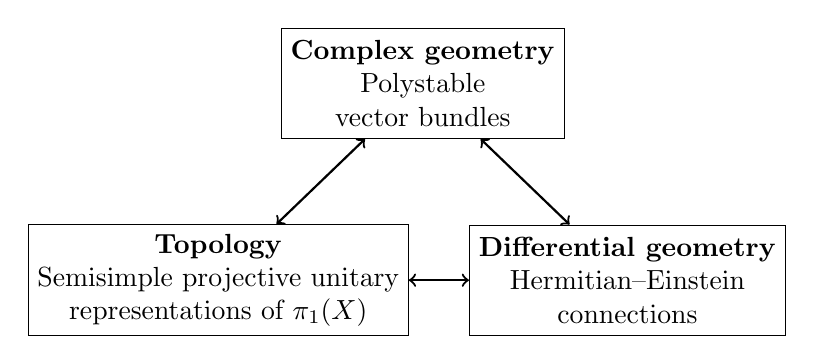
\begin{tikzpicture}[
    every node/.style={draw, rectangle, align=center, minimum width=3.5cm, minimum height=1.4cm},
    arrow/.style={<->, thick}
]

% Define the triangle nodes using polar coordinates
\node (A) at (90:1cm) {\textbf{Complex geometry}\\Polystable\\vector bundles};
\node (B) at (210:3cm) {\textbf{Topology}\\Semisimple projective unitary\\representations of $\pi_1(X)$};
\node (C) at (330:3cm) {\textbf{Differential geometry}\\Hermitian--Einstein\\connections};

% Draw arrows (bidirectional)
\draw[arrow] (A) -- (B);
\draw[arrow] (B) -- (C);
\draw[arrow] (C) -- (A);

\end{tikzpicture}
\end{center}
当我们研究 \(X\) 上稳定向量丛的模空间时，这一对应使模空间能够从不同视角交织出丰富的几何结构。

另一个推广方向是考虑拟射影情形中的对应问题。V. Mehta 与 C. S. Seshadri \cite{Me-Se} 在研究带穿孔黎曼曲面 \(X^\circ\) 的基本群酉表示时开创了这一方向，这可看作是对 Narasimhan 与 Seshadri \cite{Na-Se} 工作的推广。在他们的论文中，建立了 \(X^\circ\) 的基本群酉表示与其紧化 \(X\) 上稳定抛物丛概念之间的对应。受其启发，抛物向量丛的概念逐渐推广到更高维情形。为说明起见，我们先考虑最简单的情况。

设 \((X,\omega)\) 是一个紧 Kähler 流形，\(D\) 是一个光滑不可约除子。一个抛物丛是一个二元组
\[
F_*=(F,\mathcal F),
\]
其中 \(F\to X\) 是底层全纯向量丛，而 \(\mathcal F\) 是沿除子给定的抛物结构。抛物结构 \(\mathcal F\) 是 \(F|_D\) 上一列递降的全纯子丛过滤：
\[
F|_D = F_0 \supset F_1 \supset F_2 \supset \cdots \supset F_\ell \supset 0,
\]
并为各 \(F_i\) 赋权
\[
0\le a_i < a_{i+1} <1.
\]
我们使用下标“\(*\)”来强调抛物结构；若省略“\(*\)”而只写 \(F\)，则表示抛物丛的底层丛。与普通向量丛情形一样，抛物丛也有相应的抛物 Chern 特征、次数、关于 \(\omega\) 的斜率稳定性等概念。关于抛物丛，还有其他刻画方式，可参见例如 \cite{Bw,Iy-Si,Mo2}。更一般地，也可以定义一般除子上的抛物层。它最初由 M. Maruyama 与 K. Yokogawa \cite{Ma-Yo} 为研究模问题而引入。但在本文中，我们遵循 T. Mochizuki 在 \cite[Chapter 3]{Mo1} 中给出的定义。细节见第 2 节。

自 1990 年代以来，抛物丛吸引了大量关注。更重要也更迷人的是研究带有 Higgs 场且沿除子具有对数奇性的抛物丛，因为这会导向拟射影光滑簇上的非阿贝尔 Hodge 对应，该方向由 C. T. Simpson \cite{Si1} 开创。这个主题试图将上文“三位一体”中的对象替换为：拟射影簇上的半单局部系统、调和丛以及 Chern 类平凡的稳定抛物 Higgs 丛。J. Jost 与 K. Zuo \cite{Jo-Ka} 建立了前两类对象之间的桥梁，而 T. Mochizuki \cite{Mo3} 建立了后两类对象之间的桥梁。O. Biquard \cite{Bi} 处理了底空间为带光滑除子的 Kähler 流形的情形。若底空间为带简单正规交叉除子的 Kähler 流形，该问题仍然是开放的。如今，这一主题依然活跃，研究者试图把背景推广到带某些奇性的空间上的层，例如 Klt、Dlt 簇。当没有 Higgs 场时，这个问题也曾在不同背景下被例如 \cite{Li,Li-Nasimhan,St-Wr} 考虑。

特别地，第二作者在 \cite{Li} 中证明：对于带简单正规交叉除子 \(D\) 的紧 Kähler 流形 \((X,\omega)\)，一个抛物丛 \(F_*\) 关于 \(\omega\) 稳定，当且仅当在 \(F|_{X\setminus D}\) 上存在关于某个锥型 Kähler 度量 \(\omega_\delta\)（即在 \(D\) 附近有温和奇性的度量）的 Hermitian--Einstein 度量 \(H_\delta\)，并且 \(H_\delta\) 与抛物结构相容。作为结果，作者得到了抛物版本的 Bogomolov--Gieseker 不等式。

\subsection{目的}

值得注意的是，尽管第二作者所用的锥型度量 \(\omega_\delta\) 在流的意义下与 \(\omega\) 属于同一个上同调类，但只能得到关于 \(\omega_\delta\) 而不是 \(\omega\) 的 Hermitian--Einstein 度量，这并不十分理想。本文的目的，是将先前结果推广到半稳定抛物层的情形，并同时解决这一问题。下面简要描述我们的主要结果。

设 \(F_*\) 是与 \((X,\omega,D)\) 相关的一个秩为 \(r\) 的饱和自反抛物层。记 \(\ch_k(\cdot)\) 为抛物层的第 \(k\) 个 Chern 特征算子。与通常一样，定义抛物层 \(F_*\) 的次数为
\[
\deg_\omega(F_*):=\ch_1(F_*)\cdot \frac{[\omega]^{n-1}}{(n-1)!},
\]
其斜率定义为
\[
\mu_\omega(F_*):=\frac{\deg_\omega(F_*)}{\rank(F_*)}.
\]
我们称 \(F_*\) 关于 Kähler 度量 \(\omega\) 是 \(\mu_\omega\)-稳定（或简称 \(\omega\)-稳定）的（分别地，半稳定的），如果对任意真抛物子层 \(S_*\) 都有
\[
\mu_\omega(S_*)<(\text{分别地 } \le)\,\mu_\omega(F_*).
\]

从第 2 节可知，\(F_*\) 在一个余维至少为 3 的解析子集 \(W\) 之外是局部阿贝尔的抛物丛。记
\[
X^\circ:=X-W,\qquad \mathcal F_*:=F_*|_{X^\circ}.
\]
在本文其余部分中，我们有时将 \(F\) 简称为 \(F\) 的正则部分，而将 \(F|_{X^\circ\setminus D}\) 称作 \(F_*\) 的正则部分。

\begin{definition}
称 \(F|_{X^\circ\setminus D}\) 上的一个 Hermitian 度量 \(H\) 与抛物层 \(F_*\)（或其抛物结构）相容，如果满足下列条件：
\begin{enumerate}[label=\arabic*.]
\item
\[
\frac{\sqrt{-1}}{2\pi}\tr(F_H)
\]
表示 \(\ch_1(F_*)\)，其中 \(F_H\) 是 Chern 曲率张量。
\item 对任意真抛物子层 \(S_*\subset F_*\)，设 \(H|_{S_*}\) 为 \(S_*\) 正则部分上的诱导度量，则在流的意义下有
\[
\ch_1(S_*)\le \frac{\sqrt{-1}}{2\pi}\tr(F_{H|_{S_*}}).
\]
\end{enumerate}
如果进一步满足
\begin{itemize}
\item \(F_H\in L^2(H,\omega)\)；
\item \(\Lambda F_H\in L^\infty(H)\)，其中 \(\Lambda F_H\) 表示相对于 \(\omega\) 的收缩，
\end{itemize}
则称 \(H\) 是\textbf{可容许的}（admissible）。
\end{definition}

\begin{remark}
当 \(F_*\) 是抛物丛时，条件 2 中的不等式可以加强为等式。但在层的情形中，这是我们所能期望的最好结果。
\end{remark}

自反层上的可容许度量这一概念最早由 S. Bando 与 Y. Siu 在 \cite{B-S} 中引入，他们研究了自反层的 Kobayashi--Hitchin 问题。

\begin{definition}
设 \(F\) 是 Kähler 流形 \((X,\omega)\) 上的一个向量丛。若一个 Hermitian 度量 \(H\) 满足
\[
\sqrt{-1}\Lambda_\omega F_H-\lambda\cdot \id_F=0
\]
在整个 \(X\) 上成立，其中 \(\lambda\) 是实常数，\(\Lambda_\omega\) 是 Lefschetz 算子的伴随，则称 \(H\) 为 \textbf{Hermitian--Einstein}（H-E）度量。
\end{definition}

\begin{definition}
设 \(F\) 是 Kähler 流形 \((X,\omega)\) 上的一个向量丛。若一族由 \(t\in[0,\infty)\) 参数化的 Hermitian 度量 \(H(t)\) 满足
\[
\lim_{t\to\infty}\bigl\|\sqrt{-1}\Lambda_\omega F_{H(t)}-\lambda\cdot \id_F\bigr\|_{L^\infty(X,H(t))}=0,
\]
则称其为\textbf{近似 Hermitian--Einstein}（approximate H-E）度量族。
\end{definition}

我们得到如下定理：

\begin{theorem}[定理 6.14]
设 \(F_*\) 是 \((X,\omega,D)\) 上的一个饱和自反抛物层。则 \(F_*\) 是 \(\mu_\omega\)-多稳定的，当且仅当在 \(F|_{X^\circ\setminus D}\) 上存在一个关于 \(\omega\) 的、与 \(F_*\) 相容的可容许 H-E 度量。
\end{theorem}

\begin{theorem}[定理 6.15]
设 \(F_*\) 是 \((X,\omega,D)\) 上的一个饱和自反抛物层。则 \(F_*\) 是 \(\mu_\omega\)-半稳定的，当且仅当在 \(F|_{X^\circ\setminus D}\) 上存在一族关于 \(\omega\) 的、与 \(F_*\) 相容的可容许近似 H-E 度量。
\end{theorem}

作为推论，我们得到抛物版本的 Bogomolov--Gieseker 不等式。记
\[
\Delta(F_*):=\frac{\ch_1(F_*)^2}{2\rank(F_*)}-\ch_2(F_*)
\]
为 Bogomolov--Gieseker 判别式。

\begin{corollary}[推论 6.16]
若 \(F_*\) 关于 \(\omega\) 是 \(\mu_\omega\)-半稳定的，则
\[
\Delta(F_*)\cdot [\omega]^{n-2}\ge 0.
\]
此外，若 \(F_*\) 是多稳定的，则等号成立当且仅当 \(F|_{X\setminus D}\) 是一个向量丛，且它带有一个与抛物结构相容的射影平坦 H-E 联络。
\end{corollary}

为层建立 Bogomolov--Gieseker 不等式使我们在应用中有更大的灵活性。作为结果，我们还证明了：

\begin{theorem}[定理 7.1]
设 \(F_*\) 是紧 Kähler 流形 \((X,\omega)\) 上的一个饱和自反抛物层，并且它关于一个 nef 且 big 的类 \([\eta]\) 是半稳定的。那么关于 \([\eta]\) 的 Bogomolov--Gieseker 不等式成立，即
\[
\Delta(F_*)\cdot [\eta]^{n-2}\ge 0.
\]
\end{theorem}

\subsection{文章结构}

\begin{itemize}
\item \S2：我们引入一个以抛物层为对象的阿贝尔范畴。粗略地说，一个抛物层 \(F_*\) 是一族仅在除子 \(D\) 上退化的层过滤。我们讨论态射、Chern 特征、次数、稳定性条件等概念。我们还证明，一个饱和自反抛物层 \(F_*\) 在余维至少为 3 的解析集之外是抛物丛。

\item \S3：我们通过沿 \(W\) 上方的光滑中心连续爆破来解消 \(F_*\) 的奇性。总之，我们得到一个修改 \(\pi:\widetilde X\to X\)。设 \(E\) 为例外除子。为简化记号，我们对由 \(\pi\) 拉回的对象仍使用原记号。于是，在 \(\widetilde X\) 上，\(F\) 可以嵌入一个局部自由层 \(\mathcal E\) 中，且在 \(E\) 外 \(\mathcal E\) 与 \(F\) 同构。再经进一步爆破后，\(\mathcal E\) 将从 \(F_*\) 继承抛物结构。记该抛物丛为 \(\mathcal E_*\)。

\item \S4：为了利用 Hermitian--Yang--Mills 流来变形 \(F_*\) 正则部分上的度量，我们首先在 \(\widetilde X-D\) 上构造一族由 \(\pi^*\omega\) 导出的锥型 Kähler 度量 \(\omega^\varepsilon_\delta\)。特别地，这族度量满足一个具有统一常数的 Sobolev 型不等式。相应地，我们在 \(\mathcal E_*\) 上构造一个奇异 Hermitian 度量 \(H^\varepsilon\)，它在 \(D\) 的严格变换上退化为零。然后我们证明，\(H^\varepsilon\) 的曲率张量能像普通向量丛那样给出 \(\mathcal E_*\) 的第一与第二 Chern 特征。我们相信所构造的这个抛物度量实际上给出所有抛物 Chern 特征。由于 \(\widetilde X\) 与 \(X\) 在 \(W\) 外同构，它也诱导出 \(F_*\) 正则部分上的一个度量。正如预期，\(H^\varepsilon\) 的曲率张量将给出 \(F_*\) 的第一与第二 Chern 特征。

\item \S5：我们回顾向量丛相对于丛上的 Hermitian 度量与底流形上的 Kähler 形式的解析稳定性概念。更重要的是，我们证明 Hermitian 全纯向量丛 \((F|_{X^\circ\setminus D},H^\varepsilon)\) 的解析稳定性等价于抛物层 \(F_*\) 的稳定性。

\item \S6：我们分析相对于锥型 Kähler 度量 \(\omega^\varepsilon_\delta\) 及初始度量 \(H^\varepsilon\) 的一族 Hermitian--Yang--Mills (H-Y-M) 流，在丛 \(\mathcal E|_{\widetilde X-D}\) 上：
\[
\begin{cases}
H^{-1}\dfrac{dH}{dt}
=
-2\bigl(\sqrt{-1}\Lambda_{\omega^\varepsilon_\delta}F_H-\lambda^\varepsilon_\delta\cdot \id_F\bigr),\\[0.7em]
\det(H)=\det(H^\varepsilon),\\
H(0)=H^\varepsilon.
\end{cases}
\]
我们证明，当 \(\varepsilon,\delta\to 0\) 时，这族流收敛到定义在 \(F_*\) 正则部分上的流
\[
\begin{cases}
H^{-1}\dfrac{dH}{dt}
=
-2\bigl(\sqrt{-1}\Lambda_\omega F_H-\lambda\cdot \id_F\bigr),\\[0.7em]
\det(H)=\det(H^\varepsilon),\\
H(0)=H^\varepsilon,
\end{cases}
\]
其中
\[
\lambda:=\frac{2\pi\cdot \mu_\omega(F_*)}{\operatorname{Vol}(X,\omega)}.
\]
然后我们证明，在稳定（分别地，半稳定）条件下，该流将收敛到 \(F|_{X^\circ\setminus D}\) 上一个与 \(F_*\) 相容的可容许 H-E 度量（分别地，一族可容许近似 H-E 度量）。我们也将证明其逆命题，其中 H-E 度量的可容许性是关键。

\item \S7：作为应用，我们利用 Jordan--H\"older 过滤证明：关于 big 且 nef 类的半稳定抛物层满足 Bogomolov--Gieseker 型不等式。
\end{itemize}
\chapter{抛物层的基本概念}

本章节回顾抛物层的基本概念。这些概念可参见，例如 \cite[Chapter 3]{Mo3}、\cite[Section 2]{Iy-Si}、\cite[Section 1]{Ma-Yo}。这些文献中引入的抛物层定义略有差异，但本质思想是相似的。实际上，\cite{Iy-Si} 中讨论了文献中出现的多种定义，在限制到局部阿贝尔抛物丛时它们是等价的。本文基本遵循 \cite{Mo3} 中的定义。

设 \((X,D)\) 是一对，其中 \(X\) 是复流形，\(D=\bigcup_{i\in I}D_i\) 是一个简单正规交叉除子。我们在指标集 \(I\) 上固定一个线性排序。先引入与 \((X,D)\) 相关的抛物丛，再推广到层。如果说某个性质 \(P\) 在余维 \(k-1\) 上一般成立，意即 \(P\) 在一个余维为 \(k\) 的解析子集之外成立。

\section{抛物丛}

我们从相容过滤的概念开始。固定一个向量空间 \(V\)。

\begin{definition}
\(V\) 的一个\textbf{递减左连续过滤}是一个由 \(a\in[0,1)\) 索引的子空间族 \(\mathcal F=\{F_a\mid a\in[0,1)\}\)，满足：
\begin{enumerate}[label=\arabic*.]
\item 若 \(a\le b\)，则 \(F_a\supseteq F_b\)；
\item \(F_0=V\)，且当 \(b\) 充分接近 1 时，\(F_b=0\)；
\item 若 \(\varepsilon\) 充分小，则 \(F_{a-\varepsilon}=F_a\)。
\end{enumerate}
\end{definition}

本文中出现的所有过滤都默认为递减且左连续，因此以下统称为过滤。

给定一组滤链，即 \(F=\{{}^iF\mid i\in I\}\) 其中每个$^{i}F$都是滤链。对任意 \(J\subset I\) 及 \(\eta\in[0,1)^J\)，定义
\[
{}^JF_\eta=\bigcap_{j\in J} {}^jF_{\eta_j}.
\]

\begin{definition}
一个过滤组 \(F=\{{}^iF\mid i\in I\}\) 称为\textbf{相容的}，如果它们存在一个共同分裂，即存在一个分解
\[
V=\bigoplus_{\eta\in[0,1)^I}U_\eta
\]
使得
\[
{}^IF_\rho=\bigoplus_{\eta\ge \rho} U_\eta.
\]
\end{definition}

对于复流形 \(M\) 上的一个凝聚层 \(\mathcal{V}\)，我们以同样方式定义其子层的递减左连续过滤。若过滤 \(\mathcal F=\{\F_a\mid a\in[0,1)\}\) 的各子层都是局部自由的，且对所有 \(a\)，
\[
\Gr_a:=\F_a/\F_{>a}
\]
也局部自由，则称该过滤是在向量丛范畴中的。

\begin{definition}
一个向量丛过滤组 \(\boldsymbol{F}=\{{}^iF\mid i\in I\}\) 称为\textbf{相容的}，如果：
\begin{enumerate}[label=\arabic*.]
\item 对任意 \(x\in X\)，纤维上的过滤组 \(F_x\) 按定义 2.2 相容；
\item 对任意 \(J\subset I\) 与 \(\rho\in[0,1)^J\)，\({}^J F_\rho\) 是一个子丛。
\end{enumerate}
\end{definition}

设 \(F\) 是 \(X\) 上的一个向量丛。在每个不可约分支 \(D_i\) 上，可指定 \(F|_{D_i}\) 的一个向量丛过滤 \({}^iF\)。于是得到过滤组 \(\boldsymbol{F}=\{{}^iF\mid i\in I\}\)。对任意 \(J\subset I\)，记
\[
D_J=\bigcap_{j\in J}D_j.
\]
则 \({}^JF\) 是向量丛 \(F|_{D_J}\) 上的一组过滤。

\begin{definition}
上述二元组 \((F,\boldsymbol{F})\) 称为一个\textbf{抛物丛}，如果对所有 \(J\subset I\)，在 \(D_J\) 的任意不可约分支上，\({}^J F\) 按定义 2.3 相容。称 \(\boldsymbol{F}\) 为 \(F\) 的抛物结构。
\end{definition}

\begin{definition}
一个抛物丛 \((F,\boldsymbol{F})\) 称为\textbf{局部阿贝尔的}，如果对每个 \(x\in X\)，存在其一个邻域 \(U_x\)，使得 \((F,\mathcal F)|_{U_x}\) 在抛物层范畴中同构于若干抛物线丛的直和（见下一小节定义）。
\end{definition}

N. Borne \cite{Bo} 证明了：

\begin{theorem}
给定 \((X,D)\) 上一个抛物丛 \((F,\boldsymbol{F})\)。若由正合列
\[
0\to {}^iF_a\to F\to F|_{D_i}/{}^iF_a\to 0
\]
定义的各子层的所有交都是局部自由的，则 \((F,\boldsymbol{F})\) 是局部阿贝尔的。
\end{theorem}

\begin{remark}
若底空间是一个光滑代数簇，则 Borne 的定理更强：它说明该抛物丛在任意 Zariski 邻域中都同构于抛物线丛的直和。
\end{remark}

\section{抛物层}

设 \(\F\) 是一个无挠的 \( \mathcal O_X\)-凝聚层。

\begin{definition}
\(\F\) 上的一个\textbf{抛物结构}是一个组
\[
\boldsymbol{\F}=\{{}^i\mathcal F\mid i\in I\},
\]
其中每个 \({}^i\mathcal F_a\) 是由 \(a\in[0,1)\) 索引、长度有限 \(l_i\) 的递减左连续过滤，并满足：对任意 \(a\in[0,1)\)，
\[
{}^i\mathcal F_a\supset F(-D_i),
\]
且当 \(a\) 充分大时，
\[
{}^i\mathcal F_a=F(-D_i).
\]
\end{definition}

对于 \(D_i\) 上的过滤 \({}^i\mathcal F\)，令
\[
{}^ia=\{{}^ia_0,{}^ia_1,\dots,{}^ia_{l_i}\}
\]
表示使
\[
{}^i\Gr_{{}^ia_k}\pF\neq 0
\]
的索引递增序列。通常称这些数为 \(D_i\) 上抛物结构的\textbf{权重}。称 \(\F\) 为过滤中的\textbf{顶旗}（top flag），称 \(\F(-D_i)\) 为\textbf{柄部}（handle）。

\begin{definition}
一个\textbf{抛物层}是一个二元组
\[
\pF=(\F,\boldsymbol{\F}),
\]
其中 \(\F\) 是解析凝聚层，\(\boldsymbol{\F}\) 是其上的抛物结构。
\end{definition}

\begin{definition}
\(\pF\) 的一个\textbf{抛物子层}定义为一个商无挠子层 \(\E\)，并赋予其自然诱导的抛物结构。
\end{definition}

\begin{definition}
一个态射 \(f:\pF\to \pG\) 定义为一个层态射 \(f:\F\to \G\)，并满足对所有 \(a\in[0,1)\) 及所有 \(i\)，
\[
f({}^i\F_a)\subset {}^i\G_a.
\]
\end{definition}

记两个抛物层 \(\pF\) 与 \(\pG\) 间的态射集为
\[
\Hom(\pF,\pG).
\]

\begin{definition}
一个由抛物层构成的复形
\[
\cdots\to \pE\to \pF\to \pG\to\cdots
\]
在 \(\pF\) 处正合，当且仅当对所有 \(i,a\)，复形
\[
\cdots\to {}^i\E_a\to {}^i\F_a\to {}^i\G_a\to\cdots
\]
在 \({}^i\F_a\) 处正合。
\end{definition}

一个抛物丛按如下方式给出一个抛物层。给定抛物丛 \(F_*\)，通过正合列
\[
0\to {}^i\F_a\to F\to F|_{D_i}/{}^iF_a\to 0
\]
定义抛物结构 \({}^i\F_a\)。

反之，一个抛物层距离抛物丛有多远？下面的引理给出部分回答。

我们称一个抛物层 \(\pF\) 是\textbf{自反的}，如果 \(\F\) 是自反的。若对任意 \(i,a\)，商 \(\F/{}^i\F_a\) 都是无挠的 \(\mathcal O_{D_i}\)-模，则称 \(\pF\) 是\textbf{饱和的}。记
\[
{}^i\F_a|_{D_J}:=\ker\bigl({}^Jm^{*}({}^i\F_a)\to {}^Jm^{*}(\F)\bigr),
\]
其中 \({}^Jm\) 是 \(D_J\) 的嵌入。

\begin{lemma}
一个饱和自反抛物层的抛物结构中出现的任意若干子层的交仍然是自反的。
\end{lemma}

\begin{proof}
T. Mochizuki \cite[Proposition 3.1.2]{Mo3} 证明了所有 \({}^i\F_a\) 都是自反的。于是引理由如下事实推出：一个自反层中的两个自反子层的交仍然自反。
\end{proof}

\begin{lemma}
一个饱和自反抛物层在余维 2 上是一个局部阿贝尔的抛物丛。
\end{lemma}

\begin{proof}
记该层为 \(\pF\)。由于 \(\F\) 是自反的，它在一个余维为 3 的解析子集 \(Z_0\) 之外局部自由。对每个 \(D_i\)，由于 \(\F/{}^i\F_a\) 是无挠 \(\mathcal O_{D_i}\)-模，它在 \(D_i\) 内一个余维为 2 的解析子集 \(Z_i\) 之外局部自由。因此，在 \(\bigcup_{i\in I\cup\{0\}} Z_i\) 之外，对所有 \(i\)，\({}^i\mathcal F|_{D_i}\) 都是向量丛过滤。容易检验，对于 \(i\neq j\)，向量丛过滤 \({}^i\mathcal F|_{D_{ij}}\) 与 \({}^j\mathcal F|_{D_{ij}}\) 在 \(D_{ij}\) 内一个余维为 2 的解析子集 \(Z_{ij}\) 之外相容。因此，如果我们进一步去掉所有 \(Z_{ij}\) 以及满足 \(|J|\ge 3\) 的 \(D_J\)，则 \(\pF\) 将成为一个抛物丛。由上一个引理，所有 \({}^i\F_a\) 的交都是自反的，因此它们在一个余维为 3 的解析子集 \(Z'\) 之外局部自由。去掉 \(Z'\) 后，\(\pF\) 即成为局部阿贝尔的。
\end{proof}

\begin{lemma}
一个抛物层的自反饱和化是唯一的，它在余维 1 上与原抛物层同构。即：给定抛物层 \(\pF\)，存在唯一的饱和自反抛物层 \(\F'_{*}\) 以及一个单态射
\[
m:\F_*\to \F'_*
\]
使得 \(m\) 在余维 1 上是同构。
\end{lemma}

\begin{proof}
令 \(\F'\) 为 \(\F\) 的两次对偶。它们在一个余维为 2 的解析子集 \(Z\) 外同构。由于 \(\F'\) 是正规层，我们定义抛物结构 \(\boldsymbol{\F}_1\) 为 \(\boldsymbol{\F}|_{X\setminus Z}\) 在 \(\F'\) 中的唯一延拓。由 \cite[Theorem 2.2]{Si-Tr}，\(\boldsymbol{\F}_1\) 中的子层是凝聚的。此外，\({}^i\mathcal F\) 的顶旗是 \(\F'\)，柄部是 \(\F'(-D_i)\)。因此 \(\F'/{}^i(\mathcal F_1)_a\) 可视为 \(\mathcal O_{D_i}\)-模。最后，我们将 \(\F'/{}^i(\mathcal \F_1)_a\) 的 \(\mathcal O_{D_i}\)-挠子层在商映射下的逆像定义为 \({}^i\F'_a\)。容易验证 \(\F'_*=(\F',\boldsymbol{\F}')\) 满足要求。唯一性立即由引理 2.3 及“自反层是正规层”这一事实推出。
\end{proof}

\section{抛物 Chern 特征}

假设 \(X\) 是一个紧 Kähler 流形。

\begin{definition}
一个抛物层 \(\pF\) 的\textbf{抛物 Chern 特征} \(\ch(\F_*)\) 定义为
\[
\ch(\F_*)=
\ch(D)\,
\frac{\int_0^1\cdots\int_0^1 e^{\sum_{i=1}^k a_i[D_i]}\cdot \ch({}^{I}\F_a)\,da_1\cdots da_k}
{\int_0^1\cdots\int_0^1 e^{\sum_{i=1}^k a_i[D_i]}\,da_1\cdots da_k},
\]
其中 \(k=|I|\)，且 \(a\in [0,1)^k\)。
\end{definition}

\begin{remark}
本文中，我们使用的是 \cite{Kf} 中为紧复流形上的普通凝聚解析层提供的 Chern 特征函子；他们将光滑代数情形中的交叉理论（更精确地说，GRR 定理）推广到了光滑复解析情形。上述抛物 Chern 特征定义正是建立在他们对普通层的定义之上。然而，这一定义绝非标准。上述公式最初由 Iyer 与 Simpson 在 \cite{Iy-Si} 中针对局部阿贝尔、具有有理权重的抛物丛得到。他们证明：一对由光滑概形与简单正规交叉除子组成的 \((X,D)\) 上的局部阿贝尔抛物丛范畴，与某个关联 Deligne--Mumford 栈 \(Z\) 上的向量丛范畴等价。然后他们利用这一等价定义了局部阿贝尔抛物丛的抛物 Chern 特征，并计算出上述显式公式。但对于更一般的抛物层、甚至一般抛物丛，并没有明显理由保证上述公式仍成立。我们采用它作为定义，理由如下。

首先，这样定义的 Chern 特征具有良好的函子性质。例如，给定抛物层的短正合列
\[
0\to \E_*\to \F_*\to \G_*\to 0,
\]
有
\[
\ch(\F_*)=\ch(\E_*)+\ch(\G_*).
\]
事实上，这已经足够用于第 7 节中证明 Bogomolov--Gieseker 不等式。

更重要的是，Taher 在 \cite{Ta} 中计算表明：对于在余维 1（分别地，余维 2）上局部阿贝尔的抛物丛，第一（分别地，第二）Chern 特征有如下更具体的公式。
\end{remark}

设 \(\F_*\) 在余维 2 上是局部阿贝尔的抛物丛，例如一个饱和自反抛物层。记
\[
{}^i\Gr \F_*:=\bigoplus_{a\in[0,1)}\bigl({}^i\Gr_a\F_*:={}^i\F_a/{}^i\F_{>a}\bigr)
\]
为 \(\mathcal O_{D_i}\)-模的分次层。在 \(D_i\cap D_j\) 的任意不可约分支 \(P\) 上，定义
\[
{}^P\Gr_{(a_i,a_j)}\F_*:=
{}^P\ F_{a_i,a_j}\Big/\sum_{x>a_i,\ y>a_j} {}^P \F_{x,y}.
\]
则有
\begin{align}
\ch_1(\F_*)
&=
\ch_1(\F)+
\sum_{i\in I}\sum_{a\in[0,1)}
a\cdot \rank_{D_i}({}^i\Gr_a\F_*)\cdot [D_i],
\end{align}
以及
\begin{align}
\ch_2(\F_*)
&=
\ch_2(\F)
+\sum_{i\in I}\sum_{a\in[0,1)}
a\cdot m_{i*}\bigl(\ch_1({}^i\Gr_a\F_*)\bigr)\\
&\quad
+\frac12\sum_{i\in I}\sum_{a\in[0,1)}
a^2\cdot \rank_{D_i}({}^i\Gr_a\F_*)\cdot [D_i]^2
\nonumber\\
&\quad
+\sum_{i<j}\sum_{P\in \operatorname{Irr}(D_i\cap D_j)}
\sum_{(a_i,a_j)\in[0,1)^2}
a_i a_j \cdot \rank_P({}^P\Gr_{(a_i,a_j)}\F_*)\cdot [P].
\end{align}

\begin{remark}
上述第一 Chern 特征公式最早由 V. Mehta 与 C. S. Seshadri \cite{Me-Se} 在代数曲线上引入，随后由 M. Maruyama 与 K. Yokogawa \cite{Ma-Yo} 推广到高维抛物层。局部阿贝尔抛物丛的第二 Chern 特征公式则由第二作者 \cite[Lemma 7.3, 7.4]{Li} 利用某种沿除子退化的适配度量的曲率张量得到。之后 T. Mochizuki \cite{Mo3} 将其作为饱和自反抛物层的定义。Iyer 与 Simpson \cite{Iy-Si} 给出了局部阿贝尔抛物丛的一个一般性抛物 Chern 特征定义后，Taher \cite{Ta} 证明了这个新定义与经典定义一致。
\end{remark}

由于本文只研究自反饱和抛物层，因此本小节开头给出的 Chern 特征函子足以胜任。接下来，在下面的引理中，我们比较一个抛物层与其自反饱和化的 Bogomolov--Gieseker 判别式。

\begin{lemma}
设 \(\F'_*\) 是抛物层 \(\F_*\) 的自反饱和化，则
\[
\Delta(\F'_*)\ge \Delta(\F_*).
\]
\end{lemma}

\begin{proof}
一方面，由于它们在余维 1 上同构，\(T_a={}^{I}\F'_a/{}^{I}\F_a\) 是支撑在余维 2 解析子集上的挠层。由 \cite[Theorem 1.1]{Kf}，\(\ch_1(T_a)=0\)，而 \(\ch_2(T_a)\) 由 \(\supp T_a\) 中余维 2 的不可约分支的非负线性组合表示。

另一方面，根据公式 (1)，有
\[
\ch(\F'_*)-\ch(\F_*)
=
\ch(D)\,
\frac{\int e^{\sum a_i[D_i]}\ch(T_a)}
{\int e^{\sum a_i[D_i]}}.
\]
因此容易看出
\[
\ch_1(\F'_*)=\ch_1(\F_*),
\]
且
\[
\ch_2(\F'_*)-\ch_2(\F_*)
\]
是由 \(\supp T_a\) 中余维 2 不可约分支的非负线性组合表示的流。于是
\[
\Delta(\F'_*)\ge \Delta(\F_*).
\]
\end{proof}

抛物层的稳定性、多稳定性与半稳定性定义方式与普通层完全类似。Harder--Narasimhan 过滤与 Jordan--H\"older 过滤的存在唯一性也可以像普通层那样形式上证明。并且与普通层情形一样：

\begin{lemma}
如果抛物层 \(\F_*\) 关于某个类 \([\eta]\in H^2(X,\mathbb R)\) 是稳定的，则其自反饱和化 \(\F'_*\) 也是 \(\eta\)-稳定的。
\end{lemma}
\chapter{奇点解消}

本章节说明如何通过沿光滑中心连续爆破，把一个光滑复解析流形上的自反饱和抛物层的奇性解消掉。经过奇点解消，我们将得到一个局部阿贝尔抛物丛，其抛物度数在拉回下保持不变。

下述定理 \cite[Theorem 4.11]{grivaux2010chern} 起关键作用。

\begin{theorem}
设 \(\F\) 是复解析流形 \(X\) 上的一个解析凝聚层。则存在一个双亚纯态射
\[
\pi:\widetilde X\to X,
\]
它通过沿光滑中心连续爆破得到，使得 \(\F\) 的拉回模去挠层后是局部自由的，且挠子层支撑在例外除子上。
\end{theorem}

容易证明下述推论。

\begin{corollary}
设 \(\F\) 是局部自由层 \(\E\) 的一个子层，则存在一个双亚纯态射 \(\pi:\widetilde X\to X\)，使得 \(\pi^*(\F)\) 在 \(\pi^*(\E)\) 中的饱和化是 \(\pi^*(\E)\) 的一个子丛。
\end{corollary}

设 \(\F_*\) 是 \((X,D)\) 上的饱和自反抛物层，其中 \(X\) 是光滑复解析流形，\(D\) 是简单正规交叉除子。由定理 3.1，我们可把底层层 \(\F\) 解消成一个向量丛 \(\mathcal E\to \widetilde X\)，其中 \(\pi_1:\widetilde X\to X\) 是定理 4.1 所述的某个修改。为节省记号，即便之后继续爆破，我们仍记修改为
\[
\pi:\widetilde X\to X,
\]
而 \(\mathcal E\) 的拉回仍记作 \(\mathcal E\)。我们也约定，总是假定拉回层已经模掉挠子，并继续使用原记号表示拉回层。此外，我们也不改变在连续爆破过程中生成的例外除子不可约分支逆像的记号。\(D\)（及 \(D_i\)）的严格变换始终记作 \(D^*\)（及 \(D_i^*\)），例外除子记作 \(\E\)。不失一般性，总可假定 \(D^*\) 与 \(\E\) 横截相交。

接下来，为了获得局部阿贝尔性质，我们继续爆破，使得至多只有两个除子不可约分支的严格变换相交。限制到每个 \(D_i^*\) 上，我们有 \(\mathcal E|_{D_i^*}\) 上的一列子层滤链 \({}^i\F_a|_{D_i^*}\)。于是可以应用推论 4.2，使其成为 \(\mathcal E|_{D_i^*}\) 上的一列子丛滤链。类似地，通过进一步爆破，也可使
\[
{}^i\F_a|_{D_{ij}^*}\cap {}^j\F_b|_{D_{ij}^*}
\]
成为 \(\mathcal E|_{D_{ij}^*}\) 的一个子丛，其中 \(a,b\in[0,1)\)。于是，我们在 \(D^*\) 上得到了 \(\mathcal E\) 的一个相容抛物结构。记此局部阿贝尔抛物丛为 \(\mathcal E_*\)。

由引理 3.3、定义 3.11，可容易得到：对任意 Kähler 类 \(\omega\) 以及 \(k=1,2\)，有
\[
\ch_k(\mathcal E_*)\cdot \pi^*\omega=\ch_k(\F_*)\cdot \omega.
\]

因此有：

\begin{proposition}
设 \(\F_*\) 是一对 \((X,D)\) 上的饱和自反抛物层，其中 \(X\) 是光滑复解析流形，\(D\) 是简单正规交叉除子。则存在一个由沿光滑中心连续爆破得到的双亚纯态射
\[
\pi:\widetilde X\to X,
\]
使得拉回层 \(\pi^*(\F)\) 的无挠商 \(\mathcal E\) 在 \(D^*\) 上带有局部阿贝尔抛物结构。此外，对任意 Kähler 类 \(\omega\) 及 \(k=1,2\)，有
\[
\ch_k(\mathcal E_*)\cdot \pi^*\omega=\ch_k(\F_*)\cdot \omega.
\]
\end{proposition}
\chapter{度量的构造与分析}

本节中，我们首先在 \(X\setminus D\) 上构造一族锥型 Kähler 度量 \(\omega_\delta\)，并在 \(\widetilde X\setminus D\) 上构造一族锥型 Kähler 度量 \(\omega_{\epsilon\delta}\)。接着，我们在 \(F_*\) 的正则部分上构造一个与抛物结构相容（按定义 1.1）的 Hermitian 度量 \(\widehat{H}\)。这些度量将在第 7 节研究 H-Y-M 流时使用。

令 \(h_i\) 为 \( \mathcal O_X(D_i)\) 的一个 Hermitian 度量。记 \(\sigma_i\) 为 \( \mathcal O_X(D_i)\) 的典范截面，其关于 \(h_i\) 的范数记作 \(|\sigma_i|\)。\( \mathcal O_X(D)\) 的典范截面记作 \(\sigma\)，其范数记作 \(|\sigma|\)。假定 \(|\sigma|<1\)。与上一节相同，我们在 \(\pi:\widetilde X\to X\) 的拉回下不改变几何对象的记号。

\section{锥型 Kähler 度量}

我们在 \(X\) 上构造一族正则化度量，其极限将给出 \(X\setminus D\) 上的一个锥型 Kähler 度量 \(\omega_\delta\)。这种正则化技巧常用于处理锥型 Kähler 流形上的几何问题，参见 \cite{Ga-Hi-Pn-Mi}。对任意 \(0\le \nu\) 与 \(0<\delta<\frac12\)，定义函数
\[
\chi_{\nu\delta}(t):=
\delta\int_0^t \frac{(\nu^2+s)^\delta-\nu^{2\delta}}{s}\,ds.
\]
取某个正数 \(C>0\)，定义
\[
\omega_{\nu\delta}
:=
\omega
+
C\sum_{i\in I}\sqrt{-1}\,\partial\bar\partial \chi_{\nu\delta}f(|\sigma_i|^2).
\]

\begin{proposition}
当 \(C\) 充分小时：
\begin{itemize}
\item 若 \(0<\nu\)，则对任意 \(\delta\)，\(\omega_{\nu\delta}\) 是 \(X\) 上的 Kähler 度量；
\item 若 \(\nu=0\)，则 \(\omega_\delta:=\omega^0_\delta\) 对任意 \(\delta\) 都是 \(X\setminus D\) 上的 Kähler 度量。
\end{itemize}
\end{proposition}

\begin{proof}
直接计算得
\[
\sqrt{-1}\,\partial\bar\partial \chi_{\nu\delta}(|\sigma_i|^2)
=
\sqrt{-1}\,\delta^2(\nu^2+|\sigma_i|^2)^\delta\cdot
\frac{\langle \partial_{h_i}\sigma_i,\partial_{h_i}\sigma_i\rangle}{\nu^2+|\sigma_i|^2}
-
\sqrt{-1}\,\delta\bigl((\nu^2+|\sigma_i|^2)^\delta-\nu^{2\delta}\bigr)\cdot F_{h_i}.
\]
由以下量的一致有界性可得结论：
\[
\frac{\langle \partial_{h_i}\sigma_i,\partial_{h_i}\sigma_i\rangle}{\nu^2+|\sigma_i|^2},
\qquad
F_{h_i},
\qquad
\delta(\nu^2+|\sigma_i|^2)^\delta,
\qquad
\delta^2(\nu^2+|\sigma_i|^2)^\delta.
\]
\end{proof}

上述等式也表明，当 \(\nu\to 0\) 时，\(\omega_{\nu\delta}\) 在 \(C^\infty_{\mathrm{loc}}\)-拓扑下收敛到 \(\omega_\delta\)。\(\omega_\delta\) 在 \(D\) 上任一点附近的行为良好，具体如下，这从构造上是显然的。

\begin{lemma}
设 \(x\in D_J\)，其中 \(J\subset I\)。可取以 \(x\) 为中心的小坐标邻域，使得 \(D\) 的定义方程为
\[
z_1\cdots z_k=0.
\]
则存在正常数 \(C_1\)，使得
\[
C_1^{-1}\omega_\delta
\le
\sqrt{-1}\,\delta^2\sum_{i=1}^k \frac{dz_i\wedge d\bar z_i}{|z_i|^{2-2\delta}}
+\sqrt{-1}\,\partial\bar\partial |z|^2
\le
C_1\omega_\delta.
\]
\end{lemma}

注意，\(\omega_\delta\) 的拉回 \(\pi^*\omega_\delta\) 是 \(\widetilde X\setminus D\) 上一个退化的锥型 Kähler 度量。固定 \(\widetilde X\) 上一个归一化的 Kähler 度量 \(\omega_{\widetilde X}\)，使
\[
\int_{\widetilde X}\omega_{\widetilde X}^n=1.
\]
令
\[
\omega_{\epsilon\delta}:=\omega_\delta+\epsilon\,\omega_{\widetilde X}.
\]
则 \(\omega_{\epsilon\delta}\) 是 \(\widetilde X\setminus D\) 上的锥型 Kähler 度量。并有以下命题。

\begin{proposition}
Kähler 流形 \((\widetilde X\setminus D,\omega_{\epsilon\delta})\) 满足以下三个假设：
\begin{enumerate}[label=\arabic*.]
\item \(\widetilde X\setminus D\) 的体积一致有界，与 \(\epsilon,\delta\) 无关；
\item 存在一个 exhaustion 函数 \(\phi\)，使得 \(\sqrt{-1}\Lambda_{\omega_{\epsilon\delta}}\partial\bar\partial \phi\) 有界；
\item 若 \(f\) 是 \(\widetilde X\setminus D\) 上有界的正函数，且
\[
\Delta_{\delta\epsilon}f\le B
\]
其中 \(B\in L^p\)（\(p>n\)）为某个正函数，则
\[
\|f\|_{L^\infty}\le C_2\bigl(\|B\|_{L^p}+\|f\|_{L^1}\bigr),
\]
其中常数 \(C_2\) 与 \(\epsilon,\delta\) 无关。
\end{enumerate}
这里
\[
\Delta_{\delta\epsilon}=2\sqrt{-1}\Lambda_{\omega_{\epsilon\delta}}\partial\bar\partial
\]
是负 Laplace 算子；本文中其余地方出现的 Laplace 算子都取负号约定。
\end{proposition}

\begin{proof}
第一条直接由前一引理推出。令
\[
\phi:=\log|\sigma|.
\]
则第二条由 Poincar\'e--Lelong 公式可得。

为证明第三条，我们需要用到 \cite{Go-Ph-So-Ja} 中一个非常重要的结果，后文也将用到。设 \((X,\omega_X)\) 是一个紧 Kähler 流形，且归一化满足
\[
\int_X \omega_X^n=1.
\]
设 \(X\) 的复维数为 \(n\)。对 \(X\) 上任意 Kähler 度量 \(\omega\)，记其体积为
\[
V_\omega:=[\omega]^n,
\]
并定义相对体积密度
\[
e^{\lambda_\omega}
:=
\frac{1}{V_\omega}\frac{\omega^n}{\omega_X^n}.
\]
给定 \(p\ge 1\)，定义第 \(p\) 个 Nash--Yau 熵为
\[
N_p(\omega)
:=
\frac1{V_\omega}
\int_X
\left|
\log\left(\frac1{V_\omega}\frac{\omega^n}{\omega_X^n}\right)
\right|^p\omega^n.
\]

给定一个非负连续函数 \(\gamma\in C^0(X)\)，以及参数 \(0<A\le \infty\)、\(K>0\)，考虑 Kähler 度量空间中的子集
\[
\mathcal W:=\mathcal W(n,p,A,K,\gamma)
:=
\left\{
\omega:\ [\omega]\cdot [\omega_X]^{n-1}<A,\ N_p\le K,\ e^{\lambda_\omega}\ge \gamma
\right\}.
\]

根据\cite[Theorem 2.1]{Go-Ph-So-Ja} 得到了如下关于 \(\mathcal{W}\) 中 Kähler 度量的 Sobolev 不等式：

\begin{theorem}[一致 Sobolev 不等式]
设 \(p>n\)，且 \(\gamma\) 的零点集的 Hausdorff 维数小于 \(2n-1\)。则存在 \(q=q(n,p)>1\) 及常数
\[
C_3=C_3(n,p,A,K,\gamma,q)>0,
\]
使得对任意 \(\omega\in\mathcal W\) 及任意 \(u\in L_1^2(X)\)，均有
\[
\left(
\frac1{V_\omega}\int_X |u-\bar u|^{2q}\omega^n
\right)^{1/q}
\le
C_3\frac1{V_\omega}\int_X |\nabla u|^2\omega^n,
\]
其中
\[
\bar u:=\frac1{V_\omega}\int_X u\,\omega^n.
\]
\end{theorem}

现在回到第三条的证明。我们将把上述定理应用到 \(\widetilde X\) 上的一族度量
\[
\omega_{\epsilon\delta\nu}:=\omega_{\nu\delta}+\epsilon\omega_{\widetilde X}.
\]
这是一族 \(\widetilde X\) 上的光滑 Kähler 度量。由于 \(\omega^0_{\delta,\nu}\) 仅在例外除子 \(E\) 上退化，所以 \(\omega_{\epsilon\delta\nu}\) 可由一个零点集 Hausdorff 维数为 \(2n-2\) 的连续函数 \(\gamma\) 所支撑。为了应用上述定理，我们只需检查 Nash--Yau 熵条件。回忆 \(E\cup D\) 是简单正规交叉的。因此可取局部坐标图
\[
z=(z',z'',z'''),
\]
使得
\[
D=\bigcup_{i=1}^{k'}\{z'_i=0\},\qquad
E=\bigcup_{j=1}^{k''}\{z''_j=0\}.
\]
并可设 \(|z|<1\)。记
\[
f_{\epsilon\delta\nu}:=
\frac{(\omega_{\epsilon\delta\nu})^n}{\omega_{\widetilde X}^n}.
\]
则 \(f_{\epsilon\delta\nu}\) 要么在 \(E\) 上以 \(\prod_j |z''_j|^a\) 的速度退化到 0，要么在 \(D\) 上以 \(\prod_i |z'_i|^{-a}\) 的速度爆炸到无穷，其中 \(a>0\) 可取一致。于是若固定 \(p>n\)，有
\[
|\log(f_{\epsilon\delta\nu})|^p
\le
\frac{C_{15}}{\delta^{k'}}
\cdot
\frac{\prod_{i=1}^{k'}|z'_i|^{\delta/2}}
{\prod_{j=1}^{k''}|z''_j|^{1/2}}
\]
其中 \(C_{15}\) 与 \(\delta,\epsilon,\nu\) 无关。再由引理 5.2，
\[
|\log(f_{\epsilon\delta\nu})|^p(\omega_{\epsilon\delta\nu})^n
\le
\frac{C_{15}\delta^{k'}}
{\prod_{i=1}^{k'}|z'_i|^{2-3\delta/2}\cdot \prod_{j=1}^{k''}|z''_j|^{1/2}}.
\]
因此 \(\int |\log(f_{\epsilon\delta\nu})|^p(\omega_{\epsilon\delta\nu})^n\) 一致有界。于是可取合适的 \(p>n\)、\(A\) 和 \(K\)，使得度量族 \(\omega_{\epsilon\delta\nu}\) 属于 \(\mathcal W(n,p,A,K,\gamma)\)。由上定理可推出下面的引理。
\end{proof}

\begin{lemma}
对任意 \(f\in C_0^\infty(\widetilde X\setminus D^*)\)，以及任意锥型 Kähler 度量 \(\omega_{\epsilon\delta}\) 于 \(\widetilde X\setminus D^*\) 上，都有一致 Sobolev 不等式
\[
\|f\|_{L^q}\le C_4\|f\|_{L_1^2},
\]
其中 \(C_4\) 与 \(\epsilon,\delta\) 无关。
\end{lemma}

\begin{proof}
这是因为 \(f\) 紧支撑于 \(\widetilde X\setminus D^*\) 中，而 \(\omega_{\epsilon\delta\nu}\) 在 \(\nu\to 0\) 时以 \(C^\infty_{\mathrm{loc}}\)-拓扑收敛到 \(\omega_{\epsilon\delta}\)。
\end{proof}

现在我们可用 Moser 迭代证明命题 5.3 的第三条。设 \(f\) 是一个满足假设的有界正函数，即
\[
\Delta_{\omega_{\epsilon\delta}}f
=
\sqrt{-1}\Lambda_{\omega_{\epsilon\delta}}\partial\bar\partial f
\le B.
\]
令
\[
f_\nu:=(f+\nu\log|\sigma|)^+,\qquad 0<\nu<1.
\]
则在弱意义下有
\[
\Delta_{\omega_{\epsilon\delta}}f_\nu\le B_\nu,
\]
其中 \(B_\nu\) 在 \(\nu\to 0\) 时于 \(C^\infty\)-拓扑下收敛到 \(B\)。由于 \(f_\nu\) 属于 \(C_0^\infty(\widetilde X\setminus D^*)\) 在 Sobolev 意义下的闭包，因此可对其应用 Moser 迭代，得到估计
\[
\|f_\nu\|_{L^\infty}\le C_5(\|f_\nu\|_{L^1}+\|B_\nu\|_{L^p}),
\]
其中 \(p>n\)。令 \(\nu\to 0\) 即完成证明。 \qed

一致 Sobolev 不等式还导出相对于锥型度量族 \(\omega_{\epsilon\delta}\) 的热核的一致上界。

\begin{proposition}
设 \(K_{\epsilon\delta}\) 是相对于 \(\omega_{\epsilon\delta}\) 的热核。则对任意 \(\tau>0\)，存在与 \(\epsilon,\delta\) 无关的常数 \(C_K(\tau)\)，使得
\[
0<K_{\epsilon\delta}(x,y,t)\le
C_K(\tau)
\left(
\frac1{t^n}\exp\left(-\frac{d_{\epsilon\delta}(x,y)}{(4+\tau)t}\right)+1
\right),
\]
其中 \(d^\epsilon_\delta(\cdot,\cdot)\) 是 \(\widetilde X\setminus D^*\) 上由度量 \(\omega_{\epsilon\delta}\) 诱导的距离函数。
\end{proposition}

\begin{proof}
回忆 \(\omega_{\epsilon\delta\nu}\) 是紧流形 \(\widetilde X\) 上一族光滑度量，且满足一致 Sobolev 不等式。一方面，结合 \cite{Ch-Li} 中给出的对角热核估计和 \cite[Theorem 1.1]{GrYan} 中的高斯型热核上界估计，可得
\[
0<K^\epsilon_{\delta,\nu}(x,y,t)\le
C_K(\tau)
\left(
\frac1{t^n}\exp\left(-\frac{d_{\epsilon\delta\nu}(x,y)}{(4+\tau)t}\right)+1
\right).
\]
另一方面，容易证明当 \(\nu\to 0\) 时，\(K_{\epsilon\delta\nu}\) 在 \((\widetilde X\setminus D^*)\times (\widetilde X\setminus D^*)\) 的紧子集上一致收敛到热核 \(K_{\epsilon\delta}\)。命题得证。
\end{proof}

\section{抛物度量}

本小节的目标，是在 \(F_*\) 的正则部分上构造一个 Hermitian 度量 \(\widehat{H}\)，使其按定义 1.1 与抛物结构相容。我们还希望它在 \(X\) 上按流的意义满足
\begin{align*}
\ch_1(F_*)&=\frac{\sqrt{-1}}{2\pi}\tr(F_{\widehat{H}}),\\
\ch_1(F_*)^2&=\left(\frac{\sqrt{-1}}{2\pi}\right)^2
\tr(F_{\widehat{H}})\wedge \tr(F_{\widehat{H}}),\\
\ch_2(F_*)&=\frac12\left(\frac{\sqrt{-1}}{2\pi}\right)^2
\tr(F_{\widehat{H}}\wedge F_{\widehat{H}}).
\end{align*}

\begin{definition}
若定义在 \(F_*|_{X^\circ\setminus D}\) 上的 Hermitian 度量 \(H\) 满足上述第一条等式，则称其在余维 1 上\textbf{适配}于 \(F_*\)。若它满足上述全部等式，则称其在余维 2 上\textbf{适配}于 \(F_*\)。
\end{definition}

根据命题 3.3，只需在局部阿贝尔抛物丛
\[
\mathcal E'_*:=\mathcal E\otimes [-P_0]
\]
的正则部分上构造一个在余维 2 上适配的 Hermitian 度量 \(H_0\)。确实，一旦完成这一点，取线丛 \(\mathcal O_{\widetilde X}(P_0)\) 的一个 Hermitian 度量 \(h_{P_0}\)，则
\[
\widehat{H}:=H_0\otimes h_{P_0}
\]
就是 \(\mathcal E|_{\widetilde X\setminus D^*}\) 上的一个 Hermitian 度量，从而诱导出 \(F_*\) 正则部分上的一个度量。由于 \(\mathcal E\otimes[-P_0]\cong F\)，且奇性集余维至少为 3，易见 \(\widehat{H}\) 在余维 2 上适配于 \(F_*\)。

下面介绍构造局部阿贝尔抛物丛适配度量的一种方法。本构造中使用的记号与全文其余部分无关。首先，重要的是在除子 \(D\) 的一个小邻域内找到一个在某种意义上与抛物结构相容的丛的光滑分解。

\subsection{光滑分解}

\paragraph{局部拼接}
设 \(X\) 是一个复流形，\(D=\bigcup_{1\le i\le \ell}D_i\) 是一个简单正规交叉除子，记
\[
Y=\bigcap_{i=1}^\ell D_i,\qquad S=\{a\mid 0\le a<1\}.
\]
对每个 \(1\le i\le \ell\)，令
\[
q_i:S^\ell\to S
\]
表示投影到第 \(i\) 个分量。

设 \(F_*=(F,\mathcal F)\) 是 \(X\) 上一个局部阿贝尔抛物丛。回忆 \(\mathcal F=({}^i\mathcal F\mid i=1,\dots,\ell)\) 是 \(F|_{D_i}\) 上一组按 \(S\) 索引的全纯子丛递减过滤，并满足：
\begin{itemize}
\item 对任意 \(1\le i\le \ell\) 及 \(a\in S\)，存在 \(\epsilon>0\) 使得 \({}^iF_a={}^iF_{a-\epsilon}\)；
\item 对任意 \(P\in Y\)，存在 \(P\) 的一个邻域 \(U_P\subset X\) 以及一个全纯分解
\[
F|_{U_P}=\bigoplus_{a\in S^\ell} {}^P G_a
\]
使得
\[
\bigoplus_{q_i(a)\ge @} {}^P G_a|_{D_i\cap U_P}
=
{}^i\mathcal F|_{D_i\cap U_P}.
\]
这里符号“\(@\)”表示取值于 \([0,1)\) 的实变量，而右边被理解为左连续过滤。
\end{itemize}

设 \(X_2\subset X_1\subset X\) 为开集，且 \(X_2\) 的闭包包含于 \(X_1\) 中。假设存在一个 \(C^\infty\)-分解
\[
F|_{X_1}=\bigoplus_{a\in S^\ell} {}^1G_a
\]
并满足
\[
\bigoplus_{q_i(a)\ge @} {}^1G_a|_{D_i\cap X_1}
=
{}^i\mathcal F|_{D_i\cap X_1}.
\]

\begin{proposition}
存在 \(Y\) 的一个邻域 \(U\) 及一个 \(C^\infty\)-分解
\[
F|_U=\bigoplus_{a\in S^\ell} G_a
\]
使得：
\begin{itemize}
\item \(\bigoplus_{q_i(a)\ge @}G_a|_{D_i\cap U}={}^i\mathcal F|_{D_i\cap U}\)；
\item \(G_a|_{X_2}={}^1G_a|_{X_2}\)。
\end{itemize}
\end{proposition}

\begin{proof}
由于局部上 \(F_*\) 是抛物线丛的直和，因此存在一族开集 \(U_k\)（\(k\in\Lambda\)），满足
\[
Y\subset V:=\bigcup U_k\cup X_1,
\]
并且在每个 \(U_k\) 上存在一个 \(C^\infty\)-分解
\[
F|_{U_k}=\bigoplus_{a\in S^\ell} {}^kG_a
\]
使得
\[
\bigoplus_{q_i(a)\ge @} {}^kG_a|_{D_i\cap U_k}
=
{}^i\mathcal F|_{D_i\cap U_k}.
\]

取一组从属于覆盖 \(V=\bigcup U_k\cup X_1\) 的分片单位 \(\{\chi_k\}\cup \{\chi_{X_1}\}\)，并可假定 \(\chi_{X_1}=1\) 于 \(X_2\) 上。取一个单射
\[
\psi:S^\ell\to \mathbb C.
\]
定义
\[
f_k=\sum_{a\in S^\ell}\psi(a)\cdot \id_{{}^kG_a},
\qquad
f_{X_1}=\sum_{a\in S^\ell}\psi(a)\cdot \id_{{}^1G_a}.
\]
于是得到 \(V\) 上 \(F\) 的一个 \(C^\infty\)-自同态
\[
f=\sum_{k\in\Lambda}\chi_k f_k+\chi_{X_1}f_{X_1}.
\]

同时可得如下引理：

\begin{lemma}
\(f|_Y\) 保持 \(F|_Y\) 上的各过滤 \({}^i\mathcal F\)（\(i=1,\dots,\ell\)）。此外，在 \(\ell\Gr_a(F|_Y)\) 上的诱导自同态等于乘以 \(\psi(a)\)。
\end{lemma}

于是得到特征分解
\[
(F,f)|_Y=\bigoplus_{\alpha\in\mathbb C}(K_\alpha,\alpha\cdot \id_{K_\alpha}).
\]
存在 \(Y\) 的一个邻域 \(U\) 及分解
\[
(F,f)|_U=\bigoplus_{\alpha\in\mathbb C}(K_{U,\alpha},f_\alpha)
\]
使得 \(K_{U,\alpha}|_Y=K_\alpha\)。若 \(U\) 足够小，则 \(f_\alpha|_P\)（\(P\in U\)）的任意特征值都靠近 \(\alpha\)。特别地，可设 \(f_\alpha\) 与 \(f_\beta\)（\(\alpha\ne\beta\)）没有公共特征值。定义
\[
G_a:=K_{U,\psi(a)}.
\]
由于 \(f|_{D_i\cap U}\) 保持过滤 \({}^i\mathcal F\)，有
\[
{}^iF_b|_Y=\bigoplus_{q_i(a)\ge b}K_{\psi(a)}.
\]
从而
\[
\bigoplus_{q_i(a)\ge @}G_a|_{D_i\cap U}
=
{}^i\mathcal F|_{D_i\cap U}.
\]
又因为 \(\chi_{X_1}=1\) 于 \(X_2\) 上，所以 \(G_a|_{X_2}={}^1G_a|_{X_2}\)。
\end{proof}

\paragraph{全局分解}
借助上面的命题，很容易在 \(D\) 附近得到一个整体的 \(C^\infty\)-分解。设 \(X\) 是复流形，\(D=\bigcup_{i\in\Gamma}D_i\) 为简单正规交叉除子。对任意 \(I\subset \Gamma\)，记
\[
D_I=\bigcap_{i\in I}D_i,\qquad
\partial D_I=\bigcup_{j\in \Gamma\setminus I}(D_I\cap D_j),\qquad
D_I^\circ=D_I\setminus \partial D_I.
\]
对任意 \(I\subset J\subset \Gamma\)，令
\[
q_{I,J}:S^J\to S^I
\]
表示投影。与前面一样，设 \(F_*=(F,\mathcal F)\) 是 \(X\) 上一个抛物丛，其中 \(\mathcal F=({}^i\mathcal F\mid i\in\Gamma)\) 是其抛物结构。

\begin{proposition}
存在每个 \(D_i\) 的邻域 \(U_i\) 及 \(C^\infty\)-分解
\[
F|_{U_i}=\bigoplus_{a\in S} {}^iG_a
\]
使得：
\begin{itemize}
\item 对任意 \(b\in S\)，有
\[
\bigoplus_{a\ge b} {}^iG_a|_{D_i}={}^iF_b;
\]
\item 对任意 \(I\subset \Gamma\) 及 \(a=(a_i\mid i\in I)\in S^I\)，在
\[
U_I=\bigcap_{i\in I}U_i
\]
上定义
\[
{}^IG_a:=\bigcap_{i\in I} {}^iG_{a_i}|_{U_I},
\]
则有
\[
F|_{U_I}=\bigoplus_{a\in S^I} {}^IG_a.
\]
\end{itemize}
\end{proposition}

\begin{proof}
通过对 \(|I|\) 作递降归纳，可构造 \(D_I\) 的邻域 \(V_I\) 及分解
\[
F|_{V_I}=\bigoplus_{a\in S^I} {}^IG_a
\]
满足：
\begin{enumerate}[label=(\alph*)]
\item 对任意 \(b\in S\)，
\[
\bigoplus_{q_{i,I}(a)\ge b} {}^IG_a|_{D_i\cap V_I}
=
{}^iF_b|_{D_i\cap V_I};
\]
\item 若 \(I\subset J\)，则对任意 \(a\in S^I\)，
\[
{}^IG_a|_{V_J}
=
\bigoplus_{q_{I,J}(b)=a} {}^JG_b.
\]
\end{enumerate}

设对所有满足 \(|J|\ge k_0+1\) 的 \(J\subset \Gamma\) 已构造完毕。取 \(|I|=k_0\)。对 \(I\subset J\subset \Gamma\) 且 \(U_J\neq\emptyset\)，以及 \(a\in S^I\)，定义
\[
{}^JG_a:=\bigoplus_{q_{I,J}(b)=a} {}^JG_b.
\]
于是得到
\[
F|_{U_J}=\bigoplus_{a\in S^I} {}^JG_a.
\]
由条件 (b)，若 \(J\subset K\)，则有 \({}^JG_a|_{U_K}={}^KG_a\)。从而由 \({}^JG_a\)（\(I\subsetneq J\)）可在
\[
U_{I,1}:=\bigcup_{I\subsetneq J}U_J
\]
上得到一个 \(C^\infty\)-子丛 \({}^{1,I}G_a\)，并有分解
\[
F|_{U_{I,1}}=\bigoplus_{a\in S^I} {}^{1,I}G_a.
\]

取 \(\partial D_I\) 的一个开邻域 \(U_{I,2}\subset U_{I,1}\)，且其闭包包含于 \(U_{I,1}\) 中。由命题 5.7，存在 \(D_I\) 的一个邻域 \(V_I\) 及分解
\[
F|_{U_I}=\bigoplus_{a\in S^I} {}^IG_a
\]
使得 \(I\) 满足条件 (a)，并且
\[
{}^IG_a|_{U_{I,2}}={} ^{1,I}G_a|_{U_{I,2}}.
\]
对任意 \(J\supsetneq I\)，用 \(V_J\cap U_I\) 替换 \(V_J\)，即可得到命题结论。
\end{proof}

\subsection{度量的构造}

设 \(H_1\) 是 \(F\) 的一个 Hermitian 度量，使得：
\begin{itemize}
\item 分解
\[
F|_{U_I}=\bigoplus {}^IG_a
\]
相对于 \(H_1|_{U_I}\) 是正交的。
\end{itemize}

设 \(h^{(i)}\)（\(i\in\Gamma\)）是 \( \mathcal O_X(D_i)\) 的 Hermitian 度量。令
\[
\tau_i=h^{(i)}(1,1).
\]
可假定 \(\tau_i\equiv 1\) 于 \(X\setminus U_i\) 上。再记
\[
\tau:=\prod_{i\in\Gamma}\tau_i
\]
为 \(D\) 的典范截面的诱导平方长度。定义 \(F|_{X\setminus D_i}\) 上的自同态 \(s_i\)，满足：
\begin{itemize}
\item 在 \(X\setminus U_i\) 上，\(s_i=\id\)；
\item 在 \(U_i\) 上，
\[
s_i=\sum_{a\in S}\tau_i^{-a}\id_{{}^iG_a}.
\]
\end{itemize}
于是得到 \(F\) 上的自同态
\[
s=\prod_{i\in\Gamma} s_i,
\]
且它关于 \(H_1\) 自伴。于是定义 \(F|_{X\setminus D}\) 上的 \(C^\infty\)-Hermitian 度量 \(H_0\) 为
\[
H_0(u,v)=H_1(su,v)
\]
对任意局部截面 \(u,v\) 成立。并且可将 \(H_0\) 光滑延拓到 \(X\)。

\subsection{适配性}

由构造可知，对任意 \([\eta]\in H^{n-1,n-1}(X,\mathbb C)\)，有：

\begin{proposition}
\[
\ch_1(F_*)\cdot [\eta]
=
\frac{\sqrt{-1}}{2\pi}
\int_{X\setminus D}\tr(F_{\nabla_{H_0}})\wedge \eta.
\]
\end{proposition}

设 \(\epsilon\) 为权重间最大间隔，\(\kappa\) 为最小间隔。

设 \((U,z_1,\dots,z_n)\) 是 \(X\) 的一个全纯坐标邻域，使得
\[
D\cap U=\bigcup_{i=1}^\ell \{z_i=0\}.
\]
对 \(1\le k\le \ell\)，存在 \(\lambda(k)\in \Gamma\) 使得
\[
D_{U,\lambda(k)}:=D_{\lambda(k)}\cap U=\{z_k=0\}.
\]
记
\[
I=\{\lambda(i)\mid i=1,\dots,\ell\}.
\]
缩小 \(U\) 后可设 \(U\subset U_I\)。于是得到诱导的 \(C^\infty\)-分解
\[
F|_U=\bigoplus_{a\in S^I} {}^IG_a.
\]
对任意 \(1\le k\le \ell\) 与 \(a\in S\)，记
\[
{}^kG_a=\bigoplus_{q_{\lambda(k)}(a)=a} {}^IG_a.
\]
则有分解
\[
F|_U=\bigoplus_{a\in S} {}^kG_a. \tag{4}
\]

设 \(\iota_a\) 是从 \({}^IG_a\) 到 \(F\) 的嵌入，\(\pi_a\) 是相对于 \(H_1\) 从 \(F\) 到 \({}^IG_a\) 的正交投影。定义 \({}^IG_a\) 上的诱导联络
\[
\nabla_a:=\pi_a\circ \nabla_{H_1}\circ \iota_a.
\]
则
\[
\nabla^\dagger:=\bigoplus_a \nabla_a
\]
是保持该分解的酉联络。对任意 \(a,k\)，限制在
\[
{}^kG_a|_{D_k}={}^k\Gr_a F_*
\]
上，有 \(\nabla^\dagger=\nabla_{H_1}\)。

考虑分解
\[
\nabla_{H_1}=\nabla^\dagger+\Gamma,
\]
其中 \(\Gamma\) 是
\[
\bigoplus_{a\ne b} A^1(\Hom({}^IG_b,{}^IG_a))
\]
的一个截面。写成
\[
\Gamma=\Gamma^{1,0}+\Gamma^{0,1},
\]
并令
\[
\Gamma^{1,0}=\sum \Gamma_j^{1,0}dz_j,\qquad
\Gamma^{0,1}=\sum \Gamma_j^{0,1}d\bar z_j.
\]
又分解为
\[
\Gamma_j^{p,q}=\sum (\Gamma_j^{p,q})_{a,b},
\qquad
(\Gamma_j^{p,q})_{a,b}\in A^0(\Hom({}^IG_b,{}^IG_a)).
\]
由构造，对任意 \(j,a\)，有
\[
(\Gamma_j^{p,q})_{a,a}=0.
\]

记 \(F_\nabla\) 为联络 \(\nabla\) 的曲率张量，则有：

\begin{lemma}
\[
|F_{\nabla_{H_0}}|_{H_0}=O\bigl(\tau^{-(1+\epsilon)/2}\bigr).
\]
\end{lemma}

\begin{proof}
只需在 \(U\) 中考虑。我们有
\[
F_{\nabla_{H_1}}
=
F_{\nabla^\dagger}
+\nabla^\dagger(\Gamma)
+\Gamma\wedge \Gamma.
\]
因此
\[
F_{\nabla_{H_0}}
=
F_{\nabla_{H_1}}
+\bar\partial(s^{-1}\nabla^{1,0}_{H_1}s)
=
F_{\nabla^\dagger}
+\nabla^\dagger(\Gamma)
+\Gamma\wedge \Gamma
+\bar\partial\bigl(s^{-1}\nabla^{1,0,\dagger}s+s^{-1}[\Gamma,s]\bigr)
=
B+\bar\partial(s^{-1}\Gamma s),
\]
其中 \(B\) 光滑。记
\[
A:=s^{-1}\Gamma s.
\]
则有
\[
(\bar\partial A)_{a,b}=O(|\tau_I|^{b-a-1/2}),
\]
其中 \(\frac12\in S^I\)。由于 \(H_0\) 关于该分解是对角的，因此只需估计
\[
\left(
(\bar\partial A)_{a,b}\cdot \overline{(\bar\partial A)_{a,b}}\cdot H_{2,a,a}\cdot H_{2,b,b}^{-1}
\right)^{1/2}.
\]
简单计算得
\[
\left(
(\bar\partial A)_{a,b}\cdot \overline{(\bar\partial A)_{a,b}}\cdot H_{2,a,a}\cdot H_{2,b,b}^{-1}
\right)^{1/2}
=
O(\tau_I^{\,b-a-1/2})
=
O(\tau^{-(1+\epsilon)/2}).
\]
\end{proof}

接下来证明其在余维 2 上的适配性。

我们仍在 \(U\) 中工作，并固定 \(1\le k\le \ell\)。继续考虑上述分解
\[
\nabla_{H_1}=\nabla^\dagger+\Gamma.
\]
同样写
\[
\Gamma=\Gamma^{1,0}+\Gamma^{0,1},
\qquad
\Gamma^{1,0}=\sum \Gamma_j^{1,0}dz_j,\qquad
\Gamma^{0,1}=\sum \Gamma_j^{0,1}d\bar z_j.
\]
并写成
\[
\Gamma_j^{p,q}=\sum (\Gamma_j^{p,q})_{a,b},
\qquad
(\Gamma_j^{p,q})_{a,b}\in A^0(\Hom(G_b,G_a)).
\]
由构造，对任意 \(1\le j\le n\) 及 \(a\in S\)，仍有
\[
(\Gamma_j^{p,q})_{a,a}=0.
\]

\begin{lemma}
若 \(j\ne k\) 且 \(a<b\)，则
\[
(\Gamma_j^{0,1})_{a,b}=O(|z_k|).
\]
\end{lemma}

\begin{proof}
注意 \({}^k\mathcal F\) 是 \(F|_{D_k}\) 上按全纯子丛组成的左连续递减过滤。因此对任意 \(b\in S\)，
\[
(\Gamma_j^{0,1})|_{D_k\cap U}({}^kF_b)\subset {}^kF_{\ge b}.
\]
这便推出引理结论。
\end{proof}

由于
\[
\Gamma^{0,1}=-(\Gamma^{1,0})^{\dagger_{H_1}},
\]
于是当 \(j\ne k\) 且 \(a>b\) 时，有
\[
(\Gamma_j^{1,0})_{a,b}=O(|z_k|).
\]
因此可得：

\begin{lemma}
若 \(a>b\) 且 \(j\ne k\)，则
\[
(s^{-1}\Gamma_j^{1,0}s)_{a,b}
=
O\left(
|z_k|^{1-2\epsilon}\prod_{i\ne k}|z_i|^{-2\epsilon}
\right).
\]
若 \(a<b\)，则对任意 \(j\)，
\[
(s^{-1}\Gamma_j^{1,0}s)_{a,b}
=
O\left(
\prod_{1\le i\le \ell}|z_i|^{-2\epsilon}
\right).
\]
\end{lemma}

记 \(F_{\nabla_{H_1}}\) 为 \(\nabla_{H_1}\) 的曲率，\(F_{\nabla^\dagger}\) 为 \(\nabla^\dagger\) 的曲率，则
\[
F_{\nabla_{H_1}}=F_{\nabla^\dagger}+\nabla^\dagger(\Gamma)+\Gamma\wedge \Gamma.
\]
设
\[
\nabla^\dagger=\nabla^{1,0,\dagger}+\nabla^{0,1,\dagger}
\]
是其型分解，则
\[
s^{-1}\nabla^{1,0}_{H_1}(s)=s^{-1}\nabla^{1,0,\dagger}s+s^{-1}[\Gamma^{1,0},s].
\]
进一步
\begin{align}
\bar\partial(s^{-1}\nabla^{1,0}_{H_1}s)
&=
\nabla^{0,1,\dagger}(s^{-1}\nabla^{1,0,\dagger}s)
+\nabla^{0,1,\dagger}(s^{-1}[\Gamma^{1,0},s]) \nonumber\\
&\quad
+[\Gamma^{0,1},s^{-1}\nabla^{1,0,\dagger}s]
+[\Gamma^{0,1},s^{-1}[\Gamma^{1,0},s]]. \tag{5}
\end{align}

由于任意 \(\Hom(G_a,G_b)\)（\(a\ne b\)）的截面的迹为 0，可得
\begin{align}
\tr\bigl(F_{\nabla_{H_1}}\cdot s^{-1}\nabla^{1,0}_{H_1}s\bigr)
&=
\tr\Bigl(
F_{\nabla^\dagger}\cdot s^{-1}\nabla^{1,0,\dagger}s
+\nabla^\dagger(\Gamma)\cdot s^{-1}[\Gamma^{1,0},s]\nonumber\\
&\qquad
+(\Gamma\wedge\Gamma)\cdot(s^{-1}\nabla^{1,0,\dagger}s)
+(\Gamma\wedge\Gamma)\cdot s^{-1}[\Gamma^{1,0},s]
\Bigr). \tag{6}
\end{align}

还可得
\begin{align}
\tr\bigl(\bar\partial(s^{-1}\nabla^{1,0}_{H_1}s)\cdot s^{-1}\nabla^{1,0}_{H_1}s\bigr)
&=
\tr\bigl(\nabla^{0,1,\dagger}(s^{-1}\nabla^{1,0,\dagger}s)\cdot s^{-1}\nabla^{1,0,\dagger}s\bigr)\nonumber\\
&\quad
+\tr\bigl(\nabla^{0,1,\dagger}(s^{-1}[\Gamma^{1,0},s])\cdot s^{-1}[\Gamma^{1,0},s]\bigr)\nonumber\\
&\quad
+\tr\bigl([\Gamma^{0,1},s^{-1}\nabla^{1,0,\dagger}s]\cdot s^{-1}[\Gamma^{1,0},s]\bigr)\nonumber\\
&\quad
+\tr\bigl([\Gamma^{0,1},s^{-1}[\Gamma^{1,0},s]]\cdot s^{-1}\nabla^{1,0,\dagger}s\bigr)\nonumber\\
&\quad
+2\tr\Bigl(\Gamma^{0,1}\cdot (s^{-1}[\Gamma^{1,0},s])^2\Bigr). \tag{7}
\end{align}

注意到
\begin{align}
\tr\bigl(\nabla^{0,1,\dagger}(s^{-1}[\Gamma^{1,0},s])\cdot s^{-1}[\Gamma^{1,0},s]\bigr)
&=
\tr\bigl(s^{-1}[\nabla^{0,1,\dagger}\Gamma^{1,0},s]\cdot s^{-1}[\Gamma^{1,0},s]\bigr)\nonumber\\
&\quad
-\tr\bigl([s^{-1}\Gamma^{1,0}s,s^{-1}\nabla^{0,1,\dagger}s]\cdot s^{-1}[\Gamma^{1,0},s]\bigr), \tag{8}
\end{align}
\begin{align}
\tr\bigl([\Gamma^{0,1},s^{-1}\nabla^{1,0,\dagger}s]\cdot s^{-1}[\Gamma^{1,0},s]\bigr)
&=
-\tr\bigl(s^{-1}\nabla^{1,0,\dagger}s\cdot[\Gamma^{0,1},\Gamma^{1,0}]\bigr)\nonumber\\
&\quad
+\tr\bigl([\Gamma^{0,1},s^{-1}\Gamma^{1,0}s]\cdot s^{-1}\nabla^{1,0,\dagger}s\bigr), \tag{9}
\end{align}
\begin{align}
\tr\bigl([\Gamma^{0,1},s^{-1}[\Gamma^{1,0},s]]\cdot s^{-1}\nabla^{1,0,\dagger}s\bigr)
&=
-\tr\bigl([\Gamma^{0,1},\Gamma^{1,0}]\cdot s^{-1}\nabla^{1,0,\dagger}s\bigr)\nonumber\\
&\quad
+\tr\bigl([\Gamma^{0,1},s^{-1}\Gamma^{1,0}s]\cdot s^{-1}\nabla^{1,0,\dagger}s\bigr). \tag{10}
\end{align}

于是，对任意 2-形式 \(\tau\)，记 \(\tau^{1,1}\) 为其 \((1,1)\)-部分，可得
\begin{align}
&2\tr\bigl(F_{\nabla_{H_1}}s^{-1}\nabla^{1,0}_{H_1}s\bigr)
+\tr\bigl(\bar\partial(s^{-1}\nabla^{1,0}_{H_1}s)\nabla^{1,0}_{H_1}s\bigr)\nonumber\\
&=
\tr\Bigl(
2F_{\nabla^\dagger}^{1,1}s^{-1}\nabla^{1,0,\dagger}s
+\nabla^{0,1,\dagger}(s^{-1}\nabla^{1,0,\dagger}s)s^{-1}\nabla^{1,0,\dagger}s
\Bigr)\nonumber\\
&\quad
+\tr\Bigl(
2\nabla^\dagger(\Gamma)^{1,1}s^{-1}[\Gamma^{1,0},s]
+
2(\Gamma\wedge\Gamma)^{1,1}s^{-1}[\Gamma^{1,0},s]
\Bigr)\nonumber\\
&\quad
+\tr\Bigl(
s^{-1}[\nabla^{0,1,\dagger}\Gamma^{1,0},s]s^{-1}[\Gamma^{1,0},s]
-
[s^{-1}\Gamma^{1,0}s,s^{-1}\nabla^{0,1,\dagger}s]s^{-1}[\Gamma^{1,0},s]
\Bigr)\nonumber\\
&\quad
+2\tr\bigl([\Gamma^{0,1},s^{-1}\Gamma^{1,0}s]s^{-1}\nabla^{1,0,\dagger}s\bigr)
+2\tr\Bigl(\Gamma^{0,1}(s^{-1}[\Gamma^{1,0},s])^2\Bigr). \tag{11}
\end{align}

定义
\[
Z_{U,\lambda(k)}(\delta)
=
U\cap \{\tau_{\lambda(k)}=\delta\}\cap \bigcap_{i\ne k}\{\tau_{\lambda(i)}\ge \delta\}.
\]
给定 \([\eta]\in H^{n-2,n-2}(X,\mathbb C)\)。利用引理 5.13 及式 (11)，可得
\begin{align}
&\lim_{\delta\to 0}
\int_{Z_{U,\lambda(k)}(\delta)}
\Bigl(
2\tr(F_{\nabla_{H_1}}s^{-1}\nabla^{1,0}_{H_1}s)
+
\tr(\bar\partial(s^{-1}\nabla^{1,0}_{H_1}s)\nabla^{1,0}_{H_1}s)
\Bigr)\cdot \eta
\nonumber\\
&=
\lim_{\delta\to 0}
\int_{Z_{U,\lambda(k)}(\delta)}
\tr\Bigl(
2F_{\nabla^\dagger}^{1,1}s^{-1}\nabla^{1,0,\dagger}s
+
\nabla^{0,1,\dagger}(s^{-1}\nabla^{1,0,\dagger}s)s^{-1}\nabla^{1,0,\dagger}s
\Bigr)\cdot \eta. \tag{12}
\end{align}

令
\[
s_{\ne k}:=\prod_{i\ne k}s_i.
\]
则
\[
s=s_{\ne k}\cdot s_k=s_k\cdot s_{\ne k},
\]
从而
\[
s^{-1}\nabla^{1,0,\dagger}s
=
s_{\ne k}^{-1}\nabla^{1,0,\dagger}s_{\ne k}
+
s_k^{-1}\nabla^{1,0,\dagger}s_k. \tag{13}
\]
于是极限表达式化为
\begin{align}
&\lim_{\delta\to 0}
\int_{Z_{U,\lambda(k)}(\delta)}
\tr\Bigl(
\nabla^{0,1,\dagger}(s^{-1}\nabla^{1,0,\dagger}s)\cdot s^{-1}\nabla^{1,0,\dagger}s
\Bigr)\eta
\nonumber\\
&=
\lim_{\delta\to 0}
\int_{Z_{U,\lambda(k)}(\delta)}
\tr\Bigl(
\bigl(\nabla^{0,1,\dagger}(s_k^{-1}\nabla^{1,0,\dagger}s_k)
+\nabla^{0,1,\dagger}(s_{\ne k}^{-1}\nabla^{1,0,\dagger}s_{\ne k})\bigr)
s_k^{-1}\nabla^{1,0,\dagger}s_k
\Bigr)\cdot \eta. \tag{14}
\end{align}

定义
\[
{}^k\Omega=\sum (-a)\cdot \id_{{}^kG_a}.
\]
则有恒等式
\[
s_k^{-1}\nabla^{1,0,\dagger}(s_k)={}^k\Omega\cdot \partial \log\tau_k, \tag{15}
\]
以及
\[
\nabla^{0,1,\dagger}\bigl(s_k^{-1}\nabla^{1,0,\dagger}(s_k)\bigr)
=
{}^k\Omega\,(\partial\bar\partial \log\tau_k). \tag{16}
\]
对
\[
{}^k\Gr_aF_*={}^kF_a/{}^kF_{>a}
\]
有
\[
\tr({}^k\Omega^2)=\sum_{a\in S} a^2\,\rank({}^k\Gr_aF_*).
\]
于是极限计算为
\begin{align}
&\lim_{\delta\to 0}
\int_{Z_{U,\lambda(k)}(\delta)}
\tr\Bigl(
\nabla^{0,1,\dagger}(s_k^{-1}\nabla^{1,0,\dagger}s_k)\cdot s_k^{-1}\nabla^{1,0,\dagger}s_k
\Bigr)\cdot \eta
\nonumber\\
&=
\pm \sum_a \frac{2\pi}{\sqrt{-1}}
\int_{U\cap H_{\lambda(k)}}
a^2 \rank({}^k\Gr_aF_*)\,\partial\bar\partial(\log\tau_k)\cdot \eta. \tag{17}
\end{align}

分解
\[
F|_{D_k}=\bigoplus {}^kG_a
\]
诱导出同构
\[
F|_{D_k}\cong \bigoplus {}^k\Gr_aF_*.
\]
在此同构下，\(\nabla^\dagger\) 限制到 \(F|_{D_k\cap U}\) 与 \(\bigoplus {}^k\Gr_aF_*\) 的 Chern 联络一致。

设 \({}^kH_{1,a}\) 是由 \(H_1\) 在 \({}^k\Gr_aF_*\) 上诱导的 Hermitian 度量，则
\begin{align}
\lim_{\delta\to 0}
\int_{Z_{U,\lambda(k)}(\delta)}
\tr\Bigl(
F_{\nabla^\dagger}^{1,1}s^{-1}\nabla^{1,0,\dagger}s
\Bigr)\cdot \eta
=
\pm \sum_a \frac{2\pi}{\sqrt{-1}}
\int_{U\cap H_{\lambda(k)}}
(-a)\tr F_{\nabla^kH_{1,a}}\cdot \eta. \tag{18}
\end{align}

设 \({}^k\widetilde H_{1,a}\) 是 \(H_1\cdot s_{\ne k}\) 在 \({}^k\Gr_aF_*|_{D_k^\circ}\) 上诱导的 Hermitian 度量，则得到
\begin{align}
&\lim_{\delta\to 0}
\int_{Z_{U,\lambda(k)}(\delta)}
\tr\Bigl(
\bigl(F_{\nabla^\dagger}^{1,1}
+\nabla^{0,1,\dagger}(s_{\ne k}^{-1}\nabla^{1,0,\dagger}s_{\ne k})\bigr)
s^{-1}\nabla^{1,0,\dagger}s
\Bigr)\cdot \eta
\nonumber\\
&=
\pm \sum_a \frac{2\pi}{\sqrt{-1}}
\int_{U\cap H_{\lambda(k)}}
(-a)\tr F_{{}^k\widetilde H_{1,a}}\cdot \eta. \tag{19}
\end{align}

综上可得
\begin{align}
&\lim_{\delta\to 0}
\pm
\int_{Z_{U,\lambda(k)}(\delta)}
\Bigl(
2\tr(F_{\nabla_{H_1}}s^{-1}\nabla^{1,0}_{H_1}s)
+
\tr(\bar\partial(s^{-1}\nabla^{1,0}_{H_1}s)s^{-1}\nabla_{H_1}s)
\Bigr)\cdot \eta
\nonumber\\
&=
\sum_a \frac{2\pi}{\sqrt{-1}}
\int_{U\cap H_{\lambda(k)}}
(-a)\bigl(
\tr F_{\nabla^kH_{1,a}}
+
\tr F_{\nabla^k\widetilde H_{1,a}}
\bigr)\cdot \eta
\nonumber\\
&\quad
+
\sum_a \frac{2\pi}{\sqrt{-1}}
\int_{U\cap H_{\lambda(k)}}
a^2\rank({}^k\Gr_aF_*)\partial\bar\partial(\log\tau_k)\cdot \eta. \tag{20}
\end{align}

类似地，固定 \(1\le j,k\le \ell\)，在集合
\[
Z_{U,\lambda(j),\lambda(k)}(\delta)
=
U\cap\{\tau_{\lambda(j)}=\tau_{\lambda(k)}=\delta\}\cap
\bigcap_{i\ne j,k}\{\tau_{\lambda(i)}\ge \delta\}
\]
上分部积分并取极限，可得
\begin{align}
&\lim_{\delta\to 0}
\pm\int_{Z_{U,\lambda(j),\lambda(k)}(\delta)}
\Bigl(
2\tr(F_{\nabla_{H_1}}s^{-1}\nabla^{1,0}_{H_1}s)
+
\tr(\bar\partial(s^{-1}\nabla^{1,0}_{H_1}s)s^{-1}\nabla_{H_1}s)
\Bigr)\cdot \eta
\nonumber\\
&=
\sum_{i\in\{j,k\}}\sum_{{}^ia}
\frac{2\pi}{\sqrt{-1}}
\int_{U\cap D_{\lambda(i)}}
(-{}^ia)\bigl(
\tr F_{\nabla^iH_{1,{}^ia}}
+
\tr F_{\nabla^i\widetilde H_{1,{}^ia}}
\bigr)\cdot \eta
\nonumber\\
&\quad
+
\sum_{i\in\{j,k\}}\sum_{{}^ia}
\frac{2\pi}{\sqrt{-1}}
\int_{U\cap D_{\lambda(i)}}
({}^ia)^2\rank({}^i\Gr_aF_*)\partial\bar\partial(\log\tau_{\lambda(i)})\cdot \eta
\nonumber\\
&\quad
-
\sum_{a\in S^{(j,k)}}
(2\pi)^2
\int_{U\cap D_{j,k}}
{}^ja\cdot {}^ka\cdot \rank({}^{jk}\Gr_aF_*)\cdot \eta. \tag{21}
\end{align}

结合式 (20) 与 (21)，即可得到余维 2 适配性，即下述命题。

\begin{proposition}
\[
\ch_2(F_*)\cdot \eta
=
\frac12\left(\frac{\sqrt{-1}}{2\pi}\right)^2
\int_{X\setminus D}
\tr(F_{\nabla_{H_0}}\wedge F_{\nabla_{H_0}})\wedge \eta.
\]
\end{proposition}

现在回到我们此前的整体设定，即 \((X,D)\) 上的一个抛物层 \(F_*\)。如在本小节开头所述，我们可在 \(F_*\) 的正则部分上构造一个度量 \(\widehat{H}\)，它在余维 2 上适配于 \(F_*\)。也就是：

\begin{proposition}
\(\widehat{H}\) 在余维 2 上适配于 \(F_*\)。
\end{proposition}

此外，还可利用第 3 节中使用的爆破技巧证明下面的命题。

\begin{proposition}
\(\widehat{H}\) 在余维 1 上适配于 \(F_*\) 的任意抛物子层 \(S_*\)。
\end{proposition}

由引理 5.11 立即推出 \(\widehat{H}\) 的曲率估计：

\begin{lemma}
\[
|F_{\widehat{H}}|_{\widehat{H}}=O(|\sigma|^{-(1+\epsilon)}).
\]
\end{lemma}
\chapter{抛物稳定性与解析稳定性}

给定紧 Kähler 流形 \((X,\omega)\) 上的一个抛物层 \(\F_*\)，定义其关于 \(\omega\) 的抛物次数为
\[
\deg_\omega(\F_*):=\ch_1(\F_*)\cdot \frac{[\omega]^{n-1}}{(n-1)!},
\]
关于 \(\omega\) 的斜率为
\[
\mu_\omega(\F_*):=\frac{\deg_\omega(\F_*)}{\rank(\F_*)}.
\]

\begin{definition}[抛物稳定性]
若对任意真抛物子层 \(\Sb_*\subset \F_*\)，都有
\[
\mu_\omega(\Sb_*)<\mu_\omega(\F_*),
\]
则称 \(\F_*\) 关于 \(\omega\) 是\textbf{抛物稳定的}。
\end{definition}

接下来回顾 Simpson \cite{Si1} 对一个 Hermitian 全纯向量丛 \((E,\bar\partial,H)\) 在非必紧的 Kähler 流形 \((X^\circ,\omega)\) 上的\textbf{解析稳定性}定义。

无挠子层 \(\Sb\subset E\) 的解析次数定义为
\[
\deg_{H,\omega}(\Sb)
:=
\frac{\sqrt{-1}}{2\pi}
\int_{\Sb_{reg}}
\tr(\F_{H|_{\Sb}})\wedge \frac{\omega^{n-1}}{(n-1)!},
\]
其中 \(H|_{\Sb}\) 是 \(\Sb\) 的局部自由部分上的限制，而 \(\Sb_{reg}\) 是 \(X^\circ\) 中 \(\Sb\) 局部自由的 Zariski 开子集。解析斜率定义为
\[
\mu_{H,\omega}(\Sb):=\frac{\deg_{H,\omega}(\Sb)}{\rank(\Sb)}.
\]

注意，由 Chern--Weil 公式，
\[
\deg_{H,\omega}(\Sb)
=
\frac{\sqrt{-1}}{2\pi}
\int_{\Sb_{reg}}\tr(p_{\Sb,H}\Lambda_\omega F_H)
-
\frac{1}{2\pi}
\int_{\Sb_{reg}}|\bar\partial p_{\Sb,H}|_H^2,
\]
其中 \(p_{\Sb}\) 是 \(E\) 到 \(\Sb\) 的正交投影。因此，若要在非紧流形 \(X^\circ\) 上定义上述概念，我们需要要求
\[
F_H\in L^1(X^\circ,\omega),\qquad
p_{\Sb,H}\in L_1^2(\Sb_H),
\]
其中 \(L_1^2(\Sb_H)\) 是关于 \(H\) 自伴的 \(\En(E)\)-截面的 Sobolev 空间。

\begin{definition}[解析稳定性]
若对任意真饱和子层 \(\Sb\subset E\)，只要 \(p_{\Sb,H}\in L_1^2(\Sb_H)\)，都有
\[
\mu_{H,\omega}(\Sb)<\mu_{H,\omega}(E),
\]
则称 \(E\) 关于 \(\omega\) 与 \(H\) 是\textbf{解析稳定的}。
\end{definition}

在上一章节中，我们构造了一个度量 \(\widehat{H}\)，它对 \(\F_*\) 的任意抛物子层 \(\Sb_*\) 在余维 1 上都是适配的，并且 \(\widehat{H}\) 定义在底层层 \(\F\) 的局部自由部分
\[
\F|_{X^\circ\setminus D}
\]
上。于是应有以下命题。

\begin{proposition}
\(\F_*\) 关于 \(\omega\) 的抛物稳定性，等价于 \(\F|_{X^\circ\setminus D}\) 关于 \(\omega\) 的限制与 \(\widehat{H}\) 的解析稳定性。
\end{proposition}

\begin{proof}
假设 \(\F\) 解析稳定。对任意真抛物子层 \(\Sb_*\subset \F_*\)，\(\Sb|_{X^\circ\setminus D}\) 是 \(\F\) 的一个无挠子层。由命题 5.16 立即推出 \(\F_*\) 是抛物稳定的。

反之，假设 \(\F_*\) 抛物稳定。我们需要比较任意真饱和子层 \(\Sb\subset \F|_{X^\circ\setminus D}\)（满足 \(p_{\Sb,\widehat{H}}\in L_1^2(\Sb_{\widehat{H}})\)）的解析斜率与 \(\F|_{X^\circ\setminus D}\) 的解析斜率。由命题 4.16，只需证明：任意这样的 \(\Sb\) 都可以延拓成 \(\F_*\) 的一个抛物子层。\cite[Proposition 5.9]{Li} 已证明 \(\Sb\) 可延拓到 \(X^\circ\) 上成为 \(\F\) 的一个凝聚子层。由于 \(X\setminus X^\circ\) 是余维 3 的解析子集，且 \(\F\) 自反，因此 \(\Sb\) 还可进一步延拓为 \(\F\) 的一个凝聚子层 \(\Sb'\)。令 \(\Sb''\) 为 \(\Sb'\) 的饱和化，则 \(\Sb''_*\) 就是 \(\F_*\) 的一个抛物子层，它延拓了 \(\Sb\)。
\end{proof}

为了方便读者并供后文使用，我们把 \cite[Proposition 5.9]{Li} 的思想总结成下面的命题。为此先引入一个关于除子附近 Hermitian 度量奇性的概念。

\begin{definition}
设 \(\Delta^n\) 是以原点为中心的多圆盘，\(\Delta^*\) 是去心单位圆盘。设 \(E\) 是 \(\Delta^n\) 上平凡全纯向量丛，\(H\) 是定义于
\[
E|_{\Delta^{n-k}\times (\Delta^*)^k}
\]
上的一个可能奇异的度量。若沿除子
\[
z_{k+1}z_{k+2}\cdots z_n=0
\]
有
\[
|H|=O(|z'|^a)
\]
其中 \(a\in\mathbb R\)，\(z'=(z_{k+1},\dots,z_n)\)，则称 \(H\) 沿该除子具有\textbf{多项式阶}。
\end{definition}

于是 \cite[Proposition 5.9]{Li} 表明：

\begin{proposition}
若 \(H\) 是定义在 \(\F|_{X^\circ\setminus D}\) 上的一个 Hermitian 度量，并且它在 \(D\) 附近局部具有多项式阶，那么对任意真饱和凝聚子层 \(\Sb\subset \F|_{X^\circ\setminus D}\)，若
\[
p_{\Sb,\widehat{H}}\in L_1^2(\Sb_H),
\]
则 \(\Sb\) 可以延拓为 \(X^\circ\) 上 \(\F\) 的一个凝聚子层。
\end{proposition}
\chapter{Kobayashi--Hitchin 对应}

我们利用 H-Y-M 流来变形 \(\widehat{H}\)。我们将证明：若抛物层是稳定的（分别地，半稳定的），则在丛 \(F|_{X^\circ\setminus D}\) 上存在一个与抛物结构相容的 H-E（分别地，近似 H-E）结构。由于 \(\widehat{H}\) 只定义在 \(X^\circ-D\) 上，而我们并不完全清楚它在奇性集 \(W\) 附近的性质，因此先在 \(\widetilde X\setminus D\) 上研究 H-Y-M 流的行为；在那里 \(\widehat{H}\) 是 \(\mathcal E|_{\widetilde X\setminus D}\) 上一个良定义的度量，并且在逼近 \(D\) 时具有多项式衰减。

\section{H-Y-M 流}

对第 5 章节中在 \(\widetilde X\setminus D\) 上构造的任意锥型 Kähler 度量 \(\omega_{\varepsilon\delta}\)，考虑 H-Y-M 流
\[
H^{-1}\frac{dH}{dt}
=
-2\left(\sqrt{-1}\Lambda_{\omega_{\varepsilon\delta}}F_H-\lambda^\varepsilon_\delta\cdot \id_{\mathcal E'}\right), \tag{22}
\]
其定义在 \(\mathcal E|_{\widetilde X\setminus D}\) 上，其中
\[
\lambda^\varepsilon_\delta
:=
\frac{\sqrt{-1}}{\Vol(X,\omega_{\varepsilon\delta})}
\int_{X\setminus D^*}
\tr(F_{\widehat{H}})\wedge \frac{(\omega_{\varepsilon\delta})^{n-1}}{(n-1)!}.
\]

下面的命题由 Simpson \cite{Si1} 得到。

\begin{proposition}
设 \((\widetilde X\setminus D,\omega_{\varepsilon\delta})\) 满足命题 4.3 中的三个假设。设 \(H\) 是一个度量，满足
\[
\|\Lambda_{\omega_{\varepsilon\delta}}F_{\widehat{H}}\|_{L^\infty(\widehat{H})}\le B
\]
其中 \(B\) 为正常数。则存在唯一解 \(H(t)\) 满足 H-Y-M 流，且
\[
\det(H)=\det(\widehat{H}),\qquad H(0)=H^\varepsilon,
\]
并且在任意有限时间区间上 \(\|H\|_{L^\infty(H^\varepsilon)}\) 有界。对于此解，对所有 \(t\) 仍有
\[
\|\Lambda_{\omega_{\varepsilon\delta}}F_H\|_{L^\infty(H)}\le B.
\]
\end{proposition}

由引理 4.17，当 \(\delta\) 足够小时，有
\[
\|\Lambda_{\omega_{\varepsilon\delta}}F_{H^\varepsilon}\|_{L^\infty(H^\varepsilon)}\le B.
\]
因此可应用上面的命题，得到一族具有相同初值 \(H^\varepsilon\) 的解 \(H^\varepsilon_\delta\)。我们希望证明 \(H^\varepsilon_\delta\) 收敛到定义在丛
\[
F:=F|_{X\setminus(D\cup W)}
\]
上的 H-Y-M 流解：
\[
H^{-1}\frac{dH}{dt}
=
-2\left(\sqrt{-1}\Lambda_\omega F_H-\lambda\cdot \id_F\right), \tag{23}
\]
其中
\[
\lambda:=\frac{2\pi\cdot \mu_\omega(F_*)}{\Vol(X,\omega)}.
\]
进一步地，在抛物层稳定假设下，我们希望初始度量 \(H^\varepsilon\) 沿流变形成一个关于 \(\omega\) 的 H-E 度量。证明思路基本来自 \cite{B-S}。首先进行一些估计。

\begin{lemma}
\[
\|\Lambda^\varepsilon_\delta F_{H^\varepsilon}\|_{L^1(H^\varepsilon,\omega_{\varepsilon\delta})}\le C_6,
\]
其中 \(C_6\) 与 \(\varepsilon,\delta\) 无关。也就是说，\(\Lambda^\varepsilon_\delta F_{H^\varepsilon}\) 一致可积。
\end{lemma}

\begin{proof}
由引理 4.17，可固定 \(\varepsilon_1,\delta_1\)，使得
\[
\sqrt{-1}\tr(F_{H^\varepsilon})\le C_7\cdot \omega^{\varepsilon_1}_{\delta_1}.
\]
于是
\begin{align*}
|\Lambda^\varepsilon_\delta F_{H^\varepsilon}|\,(\omega_{\varepsilon\delta})^n
&\le
\left(
\bigl|\Lambda^\varepsilon_\delta(C_7\omega^{\varepsilon_1}_{\delta_1}\cdot I-\sqrt{-1}F_{H^\varepsilon})\bigr|
+
|C_7\Lambda^\varepsilon_\delta \omega^{\varepsilon_1}_{\delta_1}\cdot I|
\right)
(\omega_{\varepsilon\delta})^n
\\
&\le
n\tr\bigl(2C_7\omega^{\varepsilon_1}_{\delta_1}\cdot I-\sqrt{-1}F_{H^\varepsilon}\bigr)\wedge (\omega_{\varepsilon\delta})^{n-1}.
\end{align*}
对两边积分得
\begin{align*}
\int_{X\setminus D}
|\Lambda^\varepsilon_\delta F_{H^\varepsilon}|(\omega_{\varepsilon\delta})^n
&\le
n\int_{X\setminus D}
(2rC_7\omega^{\varepsilon_1}_{\delta_1}-\sqrt{-1}\tr(F_{H^\varepsilon}))\wedge (\omega_{\varepsilon\delta})^{n-1}
\\
&\le
n\int_{X\setminus D}
(2rC_7\omega_{1,\delta_1}-\sqrt{-1}\tr(F_{H^\varepsilon}))\wedge \omega_{1,\delta}^{n-1}
\\
&=
n\int_{X\setminus D}
(2rC_7\omega_1-\sqrt{-1}\tr(F_{H^\varepsilon}))\wedge \omega_1^{n-1}
\\
&=C_6.
\end{align*}
\end{proof}

若无特别说明，本文其余部分估计中的常数均默认为对 \(\varepsilon,\delta\) 一致。

沿热流 (22)，有如下不等式（参见 \cite{Do1}）：
\[
\left(\Delta^\varepsilon_\delta+\frac{\partial}{\partial t}\right)
|\Lambda^\varepsilon_\delta F_{H^\varepsilon_\delta}|_{H^\varepsilon_\delta}
\le 0,
\]
以及
\[
\left(\Delta^\varepsilon_\delta+\frac{\partial}{\partial t}\right)
|\Lambda^\varepsilon_\delta F_{H^\varepsilon_\delta}|_{H^\varepsilon_\delta}^2
\le 0.
\]
记
\[
f(t):=|\Lambda^\varepsilon_\delta F_{H^\varepsilon_\delta}|_{H^\varepsilon_\delta}.
\]

\begin{lemma}
\(\|f_t\|_{L^1}\) 与 \(\|f_t\|_{L^2}\) 随时间单调不增。
\end{lemma}

\begin{proof}
只证明 \(L^1\) 情形。若反设存在 \(t_2>t_1\)，使得
\[
\|f(t_2)\|_{L^1}=\|f(t_1)\|_{L^1}+\delta
\]
其中 \(\delta>0\)。由于 \(\|f_t\|_{L^\infty}\le B\) 且 \(|dV_{\omega_{\varepsilon\delta}}|<\infty\)，可取一个相对紧区域 \(Z\subset X\)，使
\[
B|dV_{\omega_{\varepsilon\delta}}|(X-Z)<\delta/8.
\]
于是
\[
\|f(t_2)\|_{L^1(Z)}\ge \|f(t_1)\|_{L^1(Z)}+\frac34\delta.
\]

另一方面，取一族具有光滑边界的嵌套紧区域 \(\{X_\varphi\}\)，其极限穷尽 \(X_k-D^*\)。Simpson \cite[Section 6]{Si1} 证明：解 \(H^\varepsilon_\delta\) 可由定义在 \(X_\varphi\) 上、满足 Neumann 边界条件的 H-Y-M 流解 \(H^{\varphi,\varepsilon}_\delta\) 的 \(C^\infty_{\mathrm{loc}}\)-极限得到。记
\[
f^\varphi(t):=
|\Lambda^\varepsilon_\delta F_{H^{\varphi,\varepsilon}_\delta}|_{H^{\varphi,\varepsilon}_\delta}.
\]
则
\[
\left(\Delta^\varepsilon_\delta+\frac{\partial}{\partial t}\right)f^\varphi\le 0.
\]
对 \(X_\varphi\) 积分并分部积分，再利用 Neumann 边界条件，可得
\[
\frac{\partial}{\partial t}\|f^\varphi\|_{L^1(X_\varphi)}\le 0.
\]
当 \(\varphi\to\infty\) 时，\(H^\varphi(t_i)\) 在 \(Z\) 上 \(C^\infty\)-收敛到 \(H(t_i)\)（\(i=1,2\)），故当 \(\varphi\) 足够大时，
\[
\bigl|\|f^\varphi(t_i)\|_{L^1(Z)}-\|f(t_i)\|_{L^1(Z)}\bigr|\le \delta/8.
\]
但
\[
\|f^\varphi(t_2)\|_{L^1(X_\varphi)}\le \|f^\varphi(t_1)\|_{L^1(X_\varphi)},
\]
因此
\[
\|f^\varphi(t_2)\|_{L^1(Z)}\le \|f^\varphi(t_1)\|_{L^1(Z)}+\delta/4,
\]
从而
\[
\|f(t_2)\|_{L^1(Z)}\le \|f(t_1)\|_{L^1(Z)}+\delta/2,
\]
矛盾。\(L^2\) 情形同理。
\end{proof}

作为推论，有：

\begin{lemma}
对任意 \(t\in [0,\infty)\)，有
\[
\|\Lambda^\varepsilon_\delta F_{H^\varepsilon_\delta}\|_{L^1(H^\varepsilon_\delta)}\le C_6.
\]
\end{lemma}

\begin{lemma}
对任意 \(t>0\)，有
\[
\|\Lambda^\varepsilon_\delta F_{H^\varepsilon_\delta}\|_{L^\infty(H^\varepsilon_\delta,\omega_{\varepsilon\delta})}
\le
C_8\max(t^{-1},1).
\]
\end{lemma}

\begin{proof}
回忆我们在引理 4.5 中已对测度空间 \((\widetilde X\setminus D^*,\omega_{\varepsilon\delta})\) 上紧支撑光滑函数建立了一致 Sobolev 不等式，且 Sobolev 常数与 \(\varepsilon,\delta\) 无关。可考虑函数
\[
f^\varsigma:=|\Lambda^\varepsilon_\delta F_{H^\varepsilon_\delta}|_{H^\varepsilon_\delta}
+\varsigma(\log|\sigma|^2-At),
\]
其中 \(A\) 取得足够大，以保证 \(f^\varsigma_\nu\) 是热方程的次解。随后取
\[
\phi:=\eta_a(t)^2\,(f^\varsigma_\nu)^{2a-1},\qquad a\ge 1
\]
作为抛物型 Moser 迭代的测试函数，这里 \(\eta_a(t)\) 是适当的时间截断函数。于是对任意 \(T>0\)，得到
\[
\|f^\varsigma(t)\|_{L^\infty((X\setminus D)\times [1.5T,2T])}
\le
C_8(T^{-1})
\|f^\varsigma(t)\|_{L^1((X\setminus D)\times [T,2T])}.
\]
令 \(\varsigma\to 0\) 即得引理。
\end{proof}

记
\[
B_{\omega_1}(d):=\{x\in X\mid d_{\omega_1}(x,E)<d\}.
\]
由引理 4.17 易得：在 \(B_{\omega_1}(d)^c\) 上，
\[
|\Lambda_{\omega_{\varepsilon\delta}}F_{H^\varepsilon}|_{H^\varepsilon}
\le C_9(d^{-1})|\sigma|^{-2},
\]
其中 \(C_9(d^{-1})\) 与 \(\varepsilon,\delta\) 无关。于是有：

\begin{lemma}
对任意 \(t\ge 0\)，存在常数 \(C_{10}(d^{-1})\)，使得对所有
\[
(x,t)\in B_{\omega_1}(d)^c\times [0,\infty)
\]
均有
\[
|\Lambda_{\omega_{\varepsilon\delta}}F_{H^\varepsilon_\delta}|_{H^\varepsilon_\delta}
\le
C_{10}(d^{-1})|\sigma|^{-2}.
\]
\end{lemma}

\begin{proof}
证明的关键是热核 \(K^\varepsilon_\delta\) 的一致高斯上界，而这已在命题 4.6 中得到。其余证明完全类似于 \cite[Lemma 2.2]{Li-Zh-Zh} 的做法。
\end{proof}

令
\[
h^\varepsilon_\delta:=H^\varepsilon_\delta (H^\varepsilon)^{-1}.
\]
我们知道 \(|H^\varepsilon_\delta|_{H^\varepsilon}\) 与 \(|(H^\varepsilon_\delta)^{-1}|_{H^\varepsilon}\) 都可与正量
\[
\Phi^\varepsilon_\delta
=
\log(h^\varepsilon_\delta)+\log((h^\varepsilon_\delta)^{-1})-2\rank(E)
\]
相比。并且
\[
\frac{\partial}{\partial t}\Phi^\varepsilon_\delta
\le
2\bigl(
|\Lambda_{\omega_{\varepsilon\delta}}F_{H^\varepsilon_\delta}|_{H^\varepsilon_\delta}
+
|\Lambda_{\omega_{\varepsilon\delta}}F_{H^\varepsilon}|_{H^\varepsilon}
\bigr). \tag{24}
\]
因此得到：

\begin{lemma}
对 \((x,t)\in B_{\omega_1}(d)^c\times [0,T]\)，有
\[
|H^\varepsilon_\delta|_{H^\varepsilon}\le T\,C_{11}(d^{-1})|\sigma|^{-2},
\qquad
|(H^\varepsilon_\delta)^{-1}|_{H^\varepsilon}\le T\,C_{11}(d^{-1})|\sigma|^{-2}.
\]
\end{lemma}

为了得到 H-Y-M 流的收敛，我们还需要 \cite[Proposition 1]{B-S} 中的一个命题。

\begin{proposition}
设 \(H\) 是定义在 Kähler 流形 \((Y,\omega)\) 上的一个 Hermitian 矩阵值函数，属于 Sobolev 空间 \(L_1^2\)。假设 \(H\) 与 \(H^{-1}\) 一致有界，且它在弱意义下满足椭圆方程
\[
\Lambda_\omega \bar\partial(\partial H\cdot H^{-1})=f,
\]
其中 \(f\) 一致有界。则 \(H\in C_{\mathrm{loc}}^{1,\alpha}\)（任意 \(0<\alpha<1\)），并满足仅依赖于 \(\|H\|_{L^\infty}\)、\(\|H^{-1}\|_{L^\infty}\)、\(\|f\|_{L^\infty}\) 以及 \(Y\) 的几何的估计。
\end{proposition}

现在可将上面命题应用于 \((X^\circ-D,\omega_{\varepsilon\delta})\) 上的 \(H^\varepsilon_\delta\) 做内部估计。注意 \(\omega_{\varepsilon\delta}\) 在局部上一致拟等距于固定 Kähler 度量 \(\omega_1\)。于是可简单地将 \(\Lambda_{\omega_{\varepsilon\delta}}F_{H^\varepsilon_\delta}\) 视为上命题中的 \(f\)。因此，对任意 \(t\ge 0\)，\(H^\varepsilon_\delta\) 在 \(C_{\mathrm{loc}}^{1,\alpha}\)-拓扑下一致有界。另一方面，由 H-Y-M 流方程可见，对任意 \(t>0\)，\(\frac{d}{dt}H^\varepsilon_\delta\) 在 \(C^0_{\mathrm{loc}}\)-拓扑下一致有界。故 \(H^\varepsilon_\delta\) 在 \(C^{1/0}_{\mathrm{loc}}\)-拓扑下收敛到定义在
\[
\mathcal E|_{\widetilde X\setminus D^*-\pi^{-1}(W)}
\]
上的一个时间依赖 Hermitian 度量流 \(H\)，等价地说，定义在
\[
F:=F|_{X\setminus(D\cup W)}
\]
上的流，初值为 \(H^\varepsilon\)。再利用抛物型 Schauder 估计，可知 \(H\) 实际上是一个光滑解，并且 \(H^\varepsilon_\delta\) 在 \(C_{\mathrm{loc}}^{\infty/\infty}\)-拓扑下收敛到 \(H\)。此外，由引理 (24)，对任意 \(t>0\)，\(H(t)\) 在逼近 \(D\) 时局部具有多项式衰减。

\section{对应}

\paragraph{从稳定性到 H-E 度量}
基于 H-Y-M 流 \(H(t)\)，我们希望证明：在抛物层 \(F_*\) 稳定的条件下，\(H\) 将收敛到 \(X^\circ\setminus D\) 上一个与抛物结构相容的 H-E 度量。类似地，在半稳定条件下，\(H(t)\) 将给出一族都与抛物结构相容的近似 H-E 度量。

困难在于 \(|\Lambda F_{H^\varepsilon}|_{H^\varepsilon}\) 在 \(X^\circ\setminus D\) 上并不有界，因此 Simpson \cite{Si1} 的论证不能直接套用。一个可能的想法是从正时间开始考虑 H-Y-M 流，再应用 Simpson 的结果。虽然由上面的分析可知，对任意 \(t>0\)，\(|\Lambda F_{H(t)}|_{H(t)}\) 有界，但似乎很难证明 \(F|_{X^\circ\setminus D}\) 关于 \(H(t)\) 的解析稳定性。不过这一困难已由第二作者在 \cite[Proposition 4.1]{Li-Zh-Zh} 中解决：在半稳定条件下，仍有
\[
\lim_{t\to\infty}\|\Phi(t)\|_{L^2(H(t))}=0,
\]
其中
\[
\Phi(t):=\|\sqrt{-1}\Lambda F_{H(t)}-\lambda\cdot \id_F\|_{L^2(H(t))}.
\]
这便蕴含了近似 H-E 度量的存在。实际上，
\[
\left(\frac{\partial}{\partial t}+\Delta_\omega\right)\Phi(t)^2\le 0.
\]
然后像引理 6.5 那样选取 Moser 迭代的测试函数，便得到
\[
\|\Phi(t)\|_{L^\infty(H(t))(X\setminus D\times [1.5T,2T])}
\le
C_{12}\|\Phi(t)\|_{L^2(H(t))(X\setminus D\times [T,2T])}.
\]

对于稳定情形，\cite[Proposition 4.1]{Li-Zh-Zh} 中所用的同样技巧可应用于 \(H(t)\)，以证明 \cite[Proposition 5.3]{Si1} 对 \(H(t)\) 成立，而这正是使用稳定性条件的关键估计。然后 \cite{Si1} 第 7 节中的论证即可推出 \(H(t)\) 收敛到一个 H-E 度量 \(H(\infty)\)。

因此我们只需证明：所得度量（H-E 或近似 H-E）与抛物结构相容，并且按定义 1.1 是可容许的。只需证明近似 H-E 情形，因为 H-E 情形可直接由 Fatou 引理推出。

先需要一个引理。

\begin{lemma}[{\cite[Lemma 5.2]{Si1}}]
设 \(Y\) 是一个非紧 Kähler 流形，它有一个 exhaustion 函数 \(\phi\)，满足
\[
\int_Y |\Delta \phi|<\infty.
\]
设 \(\eta\) 是一个 \((2n-1)\)-形式，满足
\[
\int_Y |\eta|^2<\infty.
\]
如果 \(d\eta\) 可积，则
\[
\int_Y d\eta=0.
\]
\end{lemma}

固定 \(X\setminus D\) 上一个沿 \(D\) 具有 cusp 奇性的 Kähler 度量 \(\omega_c\)。则体积密度函数
\[
\frac{(\omega_{\varepsilon\delta})^n}{\omega_c^n}
\]
在 \(\varepsilon,\delta\) 中一致有界。

\begin{proposition}
若 \(F_*\) 半稳定，则对任意 \(t>0\)，\(H(t)\) 与抛物结构相容。
\end{proposition}

\begin{proof}
由于
\[
\det(H^\varepsilon)=\det(H(t)),
\]
故 \(H(t)\) 在余维 1 上适配于 \(F_*\)。因此只需证明：对任意真抛物子层 \(S_*\)，都有
\[
\sqrt{-1}\int_{X^\circ\setminus D}\tr(F_{H^\varepsilon|_S})\wedge \omega^{n-1}
\le
\sqrt{-1}\int_{X^\circ\setminus D}\tr(F_{H(t)|_S})\wedge \omega^{n-1}.
\]

由第 3 节中的爆破过程可知
\[
\int_{X^\circ\setminus D^*}\tr(F_{H^\varepsilon|_S})\wedge \omega^{n-1}
=
\int_{X^\circ\setminus D}\tr(F_{H^\varepsilon|_S})\wedge \omega^{n-1}.
\]
对引理 6.2 的证明进行适当改写，可得到
\[
|\Lambda^\varepsilon_\delta F_{H^\varepsilon|_S}|(\omega_{\varepsilon\delta})^n
\le
n\tr\bigl(2C_7\omega_{1,\delta_1}\cdot I-\sqrt{-1}F_{H^\varepsilon|_S}\bigr)\wedge \omega_{1,\delta}^{n-1}.
\]
右侧积分有限且与 \(\delta\) 无关，故由广义支配收敛定理，
\[
\int_{X^\circ\setminus D}\tr(F_{H^\varepsilon|_S})\wedge \omega^{n-1}
=
\lim_{\varepsilon\to 0,\ \delta\to 0}
\int_{X^\circ\setminus D^*}\tr(F_{H^\varepsilon|_S})\wedge (\omega_{\varepsilon\delta})^{n-1}.
\]

对固定的 \(\varepsilon,\delta,t\)，记
\[
h^\varepsilon_{\delta|S}:=H^\varepsilon_\delta(t)|_S\cdot (H^\varepsilon|_S)^{-1},
\qquad
h^\varepsilon_\delta:=H^\varepsilon_\delta(t)\cdot (H^\varepsilon)^{-1}.
\]
Simpson \cite{Si1} 证明了 \(H^\varepsilon\) 与 \(H^\varepsilon_\delta(t)\) 彼此有界，且
\[
\partial h^\varepsilon_\delta\in L^2(H^\varepsilon,\omega_{\varepsilon\delta}).
\]
因此 \(h^\varepsilon_\delta\) 关于 \(H^\varepsilon\) 或 \(H^\varepsilon_\delta(t)\) 都有界。

又因为
\[
h^\varepsilon_{\delta|S}=p_{S,H^\varepsilon}\cdot h^\varepsilon_\delta \cdot \iota, \tag{25}
\]
以及
\[
p_{S,H^\varepsilon_\delta(t)}
=
(h^\varepsilon_{\delta|S})^{-1}\cdot p_{S,H^\varepsilon}\cdot h^\varepsilon_\delta, \tag{26}
\]
其中 \(\iota\) 是 \(S\) 到 \(E\) 的嵌入。所以
\[
\partial h^\varepsilon_{\delta|S}
=
\partial p_{S,H^\varepsilon}\cdot h^\varepsilon_\delta\cdot \iota
+
p_{S,H^\varepsilon}\cdot \partial h^\varepsilon_\delta\cdot \iota,
\]
从而
\[
\partial h^\varepsilon_{\delta|S}\in L^2(H^\varepsilon,\omega_{\varepsilon\delta}).
\]
再由 Chern--Weil 公式及式 (26)，
\[
\tr(F_{H^\varepsilon_\delta|_S})\wedge (\omega_{\varepsilon\delta})^{n-1}
\]
可积。

另一方面，
\[
\tr(F_{H^\varepsilon_\delta|_S})-\tr(F_{H^\varepsilon|_S})
=
\tr\bigl(\bar\partial(\partial H^\varepsilon|_S\cdot h^\varepsilon_{\delta|S}\cdot (h^\varepsilon_{\delta|S})^{-1})\bigr).
\]
而上面的论证表明
\[
\tr(\partial H^\varepsilon|_S\cdot h^\varepsilon_{\delta|S}\cdot (h^\varepsilon_{\delta|S})^{-1})
\wedge (\omega_{\varepsilon\delta})^{n-1}
\in L^2(H^\varepsilon,\omega_{\varepsilon\delta}).
\]
于是由引理 6.9，
\[
\int_{X^\circ\setminus D^*}
\tr(F_{H^\varepsilon|_S})\wedge (\omega_{\varepsilon\delta})^{n-1}
=
\int_{X^\circ\setminus D^*}
\tr(F_{H^\varepsilon_\delta|_S})\wedge (\omega_{\varepsilon\delta})^{n-1}.
\]

再用一次 Chern--Weil 公式，有
\[
\sqrt{-1}\tr(F_{H^\varepsilon_\delta|_S})\wedge (\omega_{\varepsilon\delta})^{n-1}
\le
\sqrt{-1}\tr(p_{S,H^\varepsilon_\delta}\Lambda^\varepsilon_\delta F_{H^\varepsilon_\delta})
\cdot
\frac{(\omega_{\varepsilon\delta})^n}{\omega_c^n}\cdot \omega_c^n.
\]
右侧项是一致有界的，因为 \(|\Lambda^\varepsilon_\delta F_{H^\varepsilon_\delta}|_{H^\varepsilon_\delta}\) 与 \(\frac{(\omega_{\varepsilon\delta})^n}{\omega_c^n}\) 都一致有界。对两边取极限并使用 Fatou 引理，即得所需不等式：
\[
\sqrt{-1}\int_{X^\circ\setminus D}\tr(F_{H^\varepsilon|_S})\wedge \omega^{n-1}
\le
\sqrt{-1}\int_{X^\circ\setminus D}\tr(F_{H(t)|_S})\wedge \omega^{n-1}.
\]
\end{proof}

\begin{proposition}
对任意 \(t>0\)，\(H(t)\) 是可容许的。
\end{proposition}

\begin{proof}
由引理 6.5，对任意 \(t>0\)，\(|\Lambda F_H|_H\) 在 \(X\setminus D\) 上有界。此外有
\begin{align}
-8\pi^2
\int_X \ch_2(F_*)\wedge \frac{\omega^{n-2}}{(n-2)!}
&=
\lim_{\varepsilon\to 0,\ \delta\to 0}
\int_X
\operatorname{tr}(F_{H^\varepsilon}\wedge F_{H^\varepsilon})\wedge \frac{(\omega_{\varepsilon\delta})^{n-2}}{(n-2)!}
\nonumber\\
&\ge
\lim_{\varepsilon\to 0,\ \delta\to 0}
\int_X
\operatorname{tr}(F_{H^\varepsilon_\delta(t)}\wedge F_{H^\varepsilon_\delta(t)})\wedge
\frac{(\omega_{\varepsilon\delta})^{n-2}}{(n-2)!}
\nonumber\\
&=
\lim_{\varepsilon\to 0,\ \delta\to 0}
\int_X
\Bigl(
|F_{H^\varepsilon_\delta(t)}|^2_{H^\varepsilon_\delta(t),\omega_{\varepsilon\delta}}
-
|\Lambda^\varepsilon_\delta F_{H^\varepsilon_\delta(t)}|^2_{H^\varepsilon_\delta(t)}
\Bigr)
\cdot
\frac{(\omega_{\varepsilon\delta})^n}{\omega_c^n}
\cdot
\frac{\omega_c^n}{n!}
\nonumber\\
&\ge
\int_X
\left(
|F_{H(t)}|^2_{H(t),\omega}
-
|\sqrt{-1}\Lambda_\omega F_{H(t)}|^2_{H(t)}
\right)\cdot \frac{\omega^n}{n!}. \tag{27}
\end{align}
第一步不等式来自 \cite[Lemma 7.1]{Li}，第二步不等式是相对于 \(\omega_c\) 诱导测度应用 Fatou 引理所得。因此对任意 \(t>0\)，\(F_{H(t)}\) 是平方可积的。
\end{proof}

\paragraph{从 H-E 度量到稳定性}
至此，我们已经完成了 Kobayashi--Hitchin 对应的一个方向。

为证明逆命题，设 \(H(t)\) 是一族与抛物结构相容的近似 H-E 度量，则由定义和 Chern--Weil 公式，对任意真子层 \(S_*\)，有
\[
\mu_\omega(S_*)
\le
\liminf_{t\to\infty}
\frac{\sqrt{-1}}{2\pi \rank(S)}
\int_{X\setminus D}\tr(F_{H|_S}(t))\wedge \omega^{n-1}
\le
\lim_{t\to\infty}
\frac{\sqrt{-1}}{2\pi \rank(F)}
\int_{X\setminus D}\tr(F_{H(t)})\wedge \omega^{n-1}
=
\mu_\omega(F_*).
\]
于是半稳定情形得证。

为证明多稳定情形的逆命题，先需要一个命题，它是 \cite[Theorem 2(b)]{B-S} 的一个轻微推广。

\begin{proposition}
设 \((\Delta^n,z_1,\dots,z_n)\) 为多圆盘，\(D\) 是由
\[
z_1z_2\cdots z_m=0
\]
定义的除子。设 \(S\) 是一个实余维 4、局部有限 Hausdorff 测度的闭子集。设 \(F_*\) 是 \(\Delta^n\) 上的一个饱和自反抛物层，其正则部分 \(F\) 定义在
\[
\Delta^n\setminus (D\cap S)
\]
上。若 \(F_*\) 在 \(F\) 上 admits 一个与抛物结构相容的可容许 H-E 度量 \(H\)，则 \(F\) 的任意局部截面 \(s\) 满足 \(H(s,s)\) 局部有界，且属于 \(L_{1,\mathrm{loc}}^2\)。
\end{proposition}

\begin{proof}
证明基本遵循 \cite[Section 1]{B-S}。

取沿一般方向的投影
\[
p:\Delta^n\to \Delta^{n-2},
\]
则 \(S\cap p^{-1}(0)\) 由可数多个点组成，这些点只可能在 0 处聚集。并且存在 \(\Delta^2\) 的一个紧子集 \(K\)，使得
\[
S\subset K\times \Delta^{n-2}.
\]
记
\[
X_t:=p^{-1}(t).
\]
除去 \(\Delta^{n-2}\) 中一个零测子集外，对每个 \(t\) 有：
\begin{itemize}
\item \(S_t:=X_t\cap S\) 只包含有限个点；
\item \(D_t:=D\cap p^{-1}(t)\) 是简单正规交叉除子。
\end{itemize}
令
\[
u:=\log^+(H(s,s)),\qquad u_t:=u|_{X_t}.
\]
我们在每个切片 \(X_t\) 内分析 \(u_t\)。

若 \(x_0\) 是 \(S_t\) 的一个孤立点，且不在 \(D_t\) 中，则 \cite[Section 3]{Ba} 已证明 \(u_t\) 在 \(x_0\) 附近属于 \(L_1^2\)，并在弱意义下满足
\[
\Delta_t u_t\le 4|F_t|.
\]

若 \(x_0\in D_t\)，则不失一般性，可在 \(X_t\) 中取以 \(x_0\) 为中心的局部坐标邻域 \((U_{x_0},z_1,z_2)\)，使得
\[
D_t=\{z_1z_2=0\}.
\]
由于 \(F_*\) 是饱和自反抛物层，而切片 \(U_{x_0}\) 的复维数是 2，因此知道 \(F_*|_{U_{x_0}}\) 是一个抛物丛。

另一方面，\(F|_{U_{x_0}\setminus D_t}\) 上有一个可容许 H-E 度量 \(H_t\)。来自规范理论中四维实维度、实余维 2 奇性的正则性定理（参见 \cite{Si-Si}）蕴含：如果 H-E 度量 \(H_t\) 的曲率张量 \(F_{H_t}\) 属于 \(L^2\)，则它实际上属于某个 \(L^p\)（\(p>2\)）。随后 O. Biquard \cite[Theorem 2.1]{Bi2} 证明：通过选择适当的复规范变换，\(F|_{U_{x_0}\setminus D_t}\) 可唯一延拓成 \(U_{x_0}\) 上的一个抛物丛 \(\widetilde F_*\)。特别地，对 \(\widetilde F_*\) 的任意全纯截面 \(s\)，\(|s|_{H_t}\) 有界。由延拓的唯一性可知
\[
\widetilde F_*\cong F_*|_{U_{x_0}}.
\]
因此在这种情形下也有弱不等式
\[
\Delta_t u_t\le 4|F_t|.
\]

\begin{remark}
Biquard 处理的是光滑除子情形下的延拓问题。他所选取的复规范涉及在穿孔多圆盘 \(\Delta^*\times \Delta\) 上求解 \(\bar\partial\)-问题。但这个证明很容易适配到简单正规交叉除子情形，即在 \(\Delta^*\times \Delta^*\) 上求解同样的 \(\bar\partial\)-问题。
\end{remark}

证明的其余部分完全照搬 \cite[Section 1]{B-S}。事实上，对任意包含 0 的紧区域 \(K'\subset \Delta^{n-2}\)，可利用上述不等式证明：沿投影方向的梯度 \(\nabla_t u\) 在 \(K\times K'\) 上平方可积。由于投影方向是一般的，故得到
\[
u\in L_{1,\mathrm{loc}}^2(\Delta^n).
\]
一旦知道这一点，再利用
\[
\Delta u\le 2|\Lambda F_H|
\]
及 \(\Lambda F_H\in L^\infty_{\mathrm{loc}}\)，便容易推出
\[
u\in L^\infty_{\mathrm{loc}}.
\]
\end{proof}

现在设 \(F_*\) 是一个饱和自反抛物层，它 admits 一个与抛物结构相容的可容许 H-E 度量 \(H\)。则由 \(H\) 的定义及 Chern--Weil 公式，容易得到对任意真抛物子层 \(S_*\)，均有
\[
\mu_\omega(S_*)\le \mu_\omega(F_*).
\]
若等号成立，记
\[
G_*:=\wedge^k F_*\otimes \det(S_*)^{-1}.
\]
由于 \(\det(S_*)^{-1}\) 是一个抛物线丛，因此其上存在一个与抛物结构相容的可容许 H-E 度量 \(H'\)。于是 \(G\) 的正则部分从 \(H\) 与 \(H'\) 继承一个可容许 H-E 度量 \(H''\)，并且
\[
\lambda(G)
=
\frac{2k\pi}{\Vol(X,\omega)}(\mu_\omega(F_*)-\mu_\omega(S_*))
=0.
\]
另一方面，由上述命题知道，对任意局部截面 \(s\)，\(|s|_{H''}\) 在 \(X\) 上有界且属于 \(L_1^2(X)\)。因此
\[
\Delta_\omega |s|_{H''}^2
\le
2\lambda(G)|s|_{H''}^2-2|\partial s|_{H''}^2
\le 0,
\]
从而得到 \(s\equiv C\neq 0\)。因此有全纯分裂
\[
F|_{X^\circ}=S|_{X^\circ}\oplus Q|_{X^\circ},
\]
其中 \(Q\) 是 \(F\) 的一个子层。

由于 \(W\) 的余维至少为 3，有
\[
\operatorname{Ext}^1(S,Q)\cong \operatorname{Ext}^1(S|_{X^\circ},Q|_{X^\circ}).
\]
因此
\[
F_*=S_*\oplus Q_*.
\]

于是，我们建立了如下 Kobayashi--Hitchin 对应：

\begin{theorem}
\((X,\omega,D)\) 上的一个饱和自反抛物层 \(F_*\) 是 \(\mu_\omega\)-多稳定的，当且仅当在 \(F_*|_{X^\circ\setminus D}\) 上存在一个关于 \(\omega\) 的、与 \(F_*\) 相容的可容许 H-E 度量。
\end{theorem}

\begin{theorem}
\((X,\omega,D)\) 上的一个饱和自反抛物层 \(F_*\) 是 \(\mu_\omega\)-半稳定的，当且仅当在 \(F_*|_{X^\circ\setminus D}\) 上存在一族关于 \(\omega\) 的近似 H-E 度量，并且它们都与 \(F_*\) 相容。
\end{theorem}

\begin{corollary}
若 \(F_*\) 关于 \(\omega\) 是 \(\mu_\omega\)-半稳定的，则
\[
\Delta(F_*)\cdot [\omega]^{n-2}\ge 0.
\]
此外，若 \(F_*\) 是多稳定的，则等号成立当且仅当 \(F|_{X\setminus D}\) 是一个向量丛，并带有一个与 \(F_*\) 的抛物结构相容的射影平坦 H-E 联络。
\end{corollary}

\begin{proof}
对式 (27) 中的计算稍作显然修改即可得到证明。
\end{proof}
\chapter{关于 nef 且 big 类的 Bogomolov--Gieseker 不等式}

我们在本章节中证明一个更一般的 Bogomolov--Gieseker 型不等式，即如下定理。

\begin{theorem}
设 \(F_*\) 是紧 Kähler 流形 \((X,\omega)\) 上的一个饱和自反抛物层，并且它关于一个 nef 且 big 的类 \([\eta]\) 是半稳定的。则关于 \(\eta\) 的 Bogomolov--Gieseker 不等式成立，即
\[
\Delta(F_*)\cdot [\eta]^{n-2}\ge 0.
\]
\end{theorem}

先简单回顾 nef 与 big 的定义。

\begin{definition}
若一个类 \([\eta]\in H^{k,k}(X,\mathbb R)\) 满足：对任意 \(\varepsilon>0\)，存在其代表元 \(\eta_\varepsilon\in [\eta]\)，使得
\[
\eta_\varepsilon\ge -\varepsilon \omega^k,
\]
则称 \([\eta]\) 是 \textbf{nef} 的。显然，这类构成 \(H^{k,k}(X,\mathbb R)\) 中的一个闭锥，记为 \(N^k\)。
\end{definition}

\begin{definition}
若一个类 \([\eta]\in H^{k,k}(X,\mathbb R)\) 满足：存在常数 \(\varepsilon>0\)，使得
\[
\eta\ge \varepsilon[\omega^k]
\]
在流的意义下成立，则称 \([\eta]\) 是 \textbf{big} 的。显然，这类构成 \(H^{k,k}(X,\mathbb R)\) 中的一个开锥，记为 \(B^k\)。
\end{definition}

记
\[
[\eta_\varepsilon]:=[\eta+\varepsilon\omega],
\]
其中 \(\omega\) 是一个 Kähler 类。下面引理描述了 \(F_*\) 关于 \([\eta_\varepsilon]\) 稳定性的开性。

\begin{lemma}
设一个抛物层 \(F_*\)（不必自反）关于某个类 \([\eta]\in B^1\) 是稳定的。则对充分小的 \(\varepsilon\)，\(F_*\) 关于 \([\eta_\varepsilon]\) 也是稳定的。
\end{lemma}

\begin{proof}
设 \(S_*\) 是 \(F_*\) 的一个真抛物子层。则
\[
\mu_{\eta_\varepsilon}(F_*)-\mu_{\eta_\varepsilon}(S_*)
=
\mu_\eta(F_*)-\mu_\eta(S_*)+\varepsilon\cdot \phi(\varepsilon).
\]
若我们能证明
\begin{enumerate}[label=\arabic*.]
\item \(|\phi(\varepsilon)|\le C_{12}\)；
\item \(\mu_\eta(F_*)-\mu_\eta(S_*)\ge C_{13}\)；
\end{enumerate}
其中 \(C_{12},C_{13}\) 与 \(S_*,\varepsilon\) 的选择无关，则结论成立。

先证明 \(\phi(\varepsilon)\) 的一致有界性。由于 \(\ch_1(S_*)\) 是 \(\ch_1(S)\) 与各 \(D_i\) 的线性组合，所以 \(\phi(\varepsilon)\) 是 \(\ch_1(F)\)、\(\ch_1(S)\)、各 \(D_i\) 与一族由 \(\varepsilon\) 参数化且有界的 big 类的交数的线性组合。因此只需证明如下断言：

\medskip
\noindent
给定一族有界的 big 类 \(\gamma_\varepsilon\)，当 \(S\) 与 \(\varepsilon\) 变化时，\(\ch_1(S)\cdot [\gamma_\varepsilon]\) 有一致上界。
\medskip

沿第 4 节的思路，我们可在无挠层 \(F\) 的正则部分上构造一个度量 \(H\)，它在余维 1 上适配于任意无挠子层 \(S\)（尽管那里处理的是抛物层，但该思想当然也可移植到普通层情形）。然后由 Gauss--Codazzi 公式，在流的意义下有
\[
\ch_1(S)
=
\frac{\sqrt{-1}}{2\pi}\tr(p_{S,H_0}\cdot F_{H_0})
-
\tr\bigl((\bar\partial p_{S,H_0})^\dagger\wedge \bar\partial p_{S,H_0}\bigr).
\]
于是容易看出 \(\ch_1(S)\cdot [\gamma_\varepsilon]\) 一致有界。

证明将由下一个引理完成，它蕴含了第 2 点。
\end{proof}

\begin{lemma}
设 \(F_*\) 是一个抛物层，\([\eta]\in B^1\)。定义
\[
\mu_\eta^{\max}:=\sup\{\mu_\eta(S_*)\mid S_*\subsetneq F_*\}.
\]
则 \(\mu_\eta^{\max}\) 可由某个真子层 \(S_*^{\max}\) 取得。
\end{lemma}

\begin{proof}
由 \cite[Lemma 2.2]{Ca}，可将
\[
\eta^{n-1}=\sum_{i=1}^s \lambda_i e_i
\]
写成 \(\lambda_i\ge 0\)、\(e_i\in H^{2(n-1)}(X,\mathbb Q)\) 的形式，并且每个 \(e_i\) 都可由一个严格正的流表示（不一定是 \((n-1,n-1)\)-流）。于是
\[
\ch_1(S_*)\cdot [\eta^{n-1}]
=
\sum_{i=1}^s \lambda_i \cdot \ch_1(S_*)\cdot [e_i].
\]
因为我们想取得最大斜率，所以可以限制到满足
\[
-C_{14}<\deg_\eta(S_*)
\]
的一类子层上，其中 \(C_{14}>0\)。利用上个引理中的论证，可取 \(C_{14}\) 足够大，使得对所有子层，
\[
\ch_1(S_*)\cdot [\eta^{n-1}]<C_{14}.
\]
记
\[
A:=\{S_*\subsetneq F_*,\ S_*\ne 0\mid -C_{14}<\ch_1(S_*)\cdot [\eta^{n-1}]\}.
\]
则对任意 \(S_*\in A\) 及满足 \(\lambda_i\ne 0\) 的指标 \(i\)，有
\[
-C_{15}<\ch_1(S_*)\cdot [e_i]<C_{15}.
\]
回忆
\[
\ch_1(S_*)
=
\ch_1(S)
+
\sum_{i\in I}\sum_{a\in[0,1)}
a\cdot \rank_{D_i}({}^i\Gr_aS_*)\cdot [D_i].
\]
由于 \(A\) 是抛物子层的集合，当 \(S_*\) 在 \(A\) 中变化时，上式中非平凡的抛物权重 \(a\) 只取自某个有限实数集。而 \(\ch_1(S)\) 与 \([D_i]\) 属于 \(H^2(X,\mathbb Z)\)，\(e_i\in H^{2(n-1)}(X,\mathbb Q)\)，因此当 \(S_*\in A\) 及指标 \(i\) 变化时，\(\ch_1(S_*)\cdot e_i\) 只能取有限多个值，从而 \(\ch_1(S_*)\cdot [\eta^{n-1}]\) 也只能取有限多个值。证明完成。
\end{proof}

设 \(F_*\) 是一个关于 big 类 \([\eta]\in B^1\) 半稳定的饱和自反抛物层。与普通层情形一样，可证明存在 Jordan--H\"older 过滤
\[
0=F_{0*}\subset F_{1*}\subset F_{2*}\subset \cdots \subset F_{n*}=F_*,
\]
其中对每个 \(0\le i<n\)，\(F_{i*}\) 是饱和自反抛物层，商
\[
\Gr_iF_*:=F_{i+1,*}/F_{i*}
\]
是一个 \(\eta\)-稳定抛物层，且
\[
\mu_\eta(\Gr_iF_*)=\mu_\eta(F_*).
\]
于是由引理 7.2 立刻得到：存在 \(\varepsilon_0\)，使得对任意 \(0<\varepsilon<\varepsilon_0\)，商 \(F_{i+1,*}/F_{i*}\) 是 \(\eta_\varepsilon\)-稳定的。

\begin{proof}[定理 7.1 的证明]
\(F_{0*}\) 是一个关于 \(\eta_\varepsilon\) 稳定的饱和自反抛物层。在 \(\eta\) 是 nef 且 big 的假设下，\(\eta_\varepsilon\) 是一个 Kähler 度量。因此
\[
\Delta(F_{0*})\cdot [\eta_\varepsilon]^{n-1}\ge 0,
\]
从而令 \(\varepsilon\to 0\) 得
\[
\Delta(F_{0*})\cdot [\eta]^{n-1}\ge 0.
\]
另一方面，由引理 2.9，\(\Gr_iF_*\) 的自反饱和化 \(\Gr_iF'_*\) 也是 \(\eta_\varepsilon\)-稳定的。再由引理 2.8，
\[
\Delta(\Gr_iF_*)\cdot [\eta]^{n-1}
\ge
\Delta(\Gr_iF'_*)\cdot [\eta]^{n-1}
\ge 0.
\]

因此只需说明：若存在抛物层的短正合列
\[
0\to F_{i*}\to F_{i+1,*}\to \Gr_iF_*\to 0,
\]
并且
\[
\Delta(F_{i*})\cdot [\eta]^{n-1}\ge 0,\qquad
\Delta(\Gr_iF_*)\cdot [\eta]^{n-1}\ge 0,
\]
则可推出
\[
\Delta(F_{i+1,*})\cdot [\eta]^{n-1}\ge 0.
\]
但这是一条标准事实，参见 \cite[Lemma 3.7]{Cl}。
\end{proof}
% \include{chapters/floats}
% \include{chapters/math}
% \include{chapters/citations}

\bibliography{bib/bibliography}  % 参考文献使用 BibTeX 编译
% \printbibliography       % 参考文献使用 BibLaTeX 编译

\appendix
% !TEX root = ../main.tex

\chapter{}
本文的证明中使用了Simpson~\cite[Section~5]{Si1}中关于Danaldson泛函在非紧流形上的定义。Simpson在证明~\cite[Proposition~5.1]{Si1}当中声称证明该命题只需证明两个恒等式即可，但是这并不是显而易见的。笔者补充了其中的细节。

Donaldson 泛函用于研究当 \(t\to\infty\) 时解 \(H_t\) 的行为。我们在此对其作一简要回顾。固定 向量丛 \(E\) 上的初始度量 \(K_0\)，令 \(S_{K_0}\) 表示相对于 \(K_0\) 的自伴随自同态所构成的实向量丛。记 \(P(S_{K_0})\) 为光滑截面 \(s\in S_{K_0}\) 所成的赋范向量空间，其范数定义为
\[
\|s\|_P=\sup_X |s|+\|\bar\partial s\|_{L^2}+\|\Delta'_{K_0}s\|_{L^1},
\]
其中 \(\Delta'_{K_0}\) 是关于 \(\partial_{K_0}\) 的 Hodge--Laplace 算子。

一个光滑函数 \(\psi:\mathbb{R}\to\mathbb{R}\) 诱导一个映射
\[
S_{K_0}\to S_{K_0},
\]
其定义如下：在 \(X\) 的每一点，取 \(E\) 的一个酉标架 \(\{e_i\}\)，使得
\[
s(e_i)=\lambda_i e_i,
\]
并定义
\[
\psi(s)(e_i)=\psi(\lambda_i)e_i.
\]

类似地，一个光滑函数 \(\Psi:\mathbb{R}\times\mathbb{R}\to\mathbb{R}\) 诱导一个映射
\[
S_{K_0}\to S_{K_0}(\En(E))
\]
如下定义：令 \(\{\hat e_i\}\) 为对偶基。对任意 \(A\in \En(E)\)，写成
\[
A=\sum_{i,j} a_{i,j}\,\hat e_i\otimes e_j.
\]
然后定义
\[
\Psi(s)(A)=\sum_{i,j}\Psi(\lambda_i,\lambda_j)a_{i,j}\,\hat e_i\otimes e_j.
\]

事实上，这样定义非线性算子 \(\Psi\) 是很自然的。设我们希望对 \(\psi(s)\) 施加 \(\bar\partial\)。若将差商 \(d\psi:\mathbb{R}\times\mathbb{R}\to\mathbb{R}\) 定义为
\[
d\psi(x,y)=\frac{\psi(x)-\psi(y)}{x-y},
\]
那么就有如下链式法则等式：
\[
\bar\partial\psi(s)=d\psi(s)(\bar\partial s). 
\]

令 \(\mathcal P\) 表示满足
\[
\int_X |\Lambda_\alpha F_K|_K<\infty
\]
的光滑 Hermitian 度量 \(K\) 的空间。Simpson在~\cite[Section~4]{Si1}中证明了$\mathcal P$是一个解析Banach流形。指数映射
\[
\exp:P(S_{K_0})\to P,\qquad s\mapsto K_0e^s,
\]
可视为解析流形 \(\mathcal P\) 在 \(K_0\) 处的一张局部坐标图。此映射的像是 \(\mathcal P\) 中包含 \(K_0\) 的一个连通分支，记为 \(\mathcal{P}_0\)。

从启发式角度看，Donaldson 泛函是定义在无限维空间 \(\mathcal P\) 上的一个势函数。若取 \(K_0\) 作为势函数的基点，则对任意 \(H\in \mathcal{P}_0\)，可写
\[
H=K_0e^s,
\]
此时 Donaldson 泛函为
\[
M(K_0,H)
=
\sqrt{-1}\int_X \tr(s\Lambda_\alpha F_{K_0})
+\int_X \{\Psi(s)(\bar\partial s),\bar\partial s\}_{K_0,\omega_\alpha},
\]
其中
\[
\Psi(x,y)=\frac{e^{\,y-x}-(y-x)-1}{(y-x)^2}.
\]

\begin{proposition}[{\cite[Proposition~5.1]{Si1}}]
    对任意位于同一连通分支 \(\mathcal{P}_0\) 中的三点 \(K,H,J\)，都有
\[
M(K,H)+M(H,J)=M(K,J).
\]

Simpson在该命题的证明中声称只需验证
\[
\frac{\partial^2}{\partial t_1\partial t_2}
M\bigl(Ke^{t_1s_1},Ke^{t_1s_1}e^{t_2s_2}\bigr)
=
\frac{\partial^2}{\partial t_1\partial t_2}
M\bigl(K,Ke^{t_1s_1}e^{t_2s_2}\bigr)
\]
在$t_1=t_2=0$处成立，以及
\[
\frac{\partial^2}{\partial t^2}M(K,Ke^{ts})
=
\frac{\partial^2}{\partial t\,\partial u}M\bigl(K,Ke^{(t+u)s}\bigr)
\]
在t=1，u=0处成立即可，但是这并不显然。我们证明上述条件的充分性。
\begin{proof}
先考虑第二个条件：
\[
\frac{\partial^2}{\partial t^2}M(K,Ke^{ts})
=
\left.\frac{\partial^2}{\partial t\,\partial u}M\bigl(K,Ke^{(t+u)s}\bigr)\right|_{t=1,u=0}.
\]
由于伸缩与平移的不变性（因为
\[
e^{(t+u)s}=e^{ts}e^{us},
\]
（注意而当矩阵 \(s\) 不同时这一点不成立）。我们可以把这部分问题归结为研究一个二元实函数 \(f(x,y)\)，它满足
\[
\frac{\partial^2}{\partial t^2}f(x,x+t)
=
\left.\frac{\partial^2}{\partial t\,\partial u}f(x+t,x+t+u)\right|_{u=0}
\]
对任意 \(x,t\) 都成立。

我们来计算：
\[
\left.\frac{\partial}{\partial u}f(x+t,x+t+u)\right|_{u=0}
=
f_y(x,x+t),
\]
其中
\[
f_y:=\frac{\partial}{\partial y}f(x,y),
\]
其余偏导记号类似。

因此，上式右端等于
\[
\frac{\partial}{\partial t}f_y(x+t,x+t)
=
f_{xy}(x+t,x+t)+f_{yy}(x+t,x+t).
\]
而左端则是
\[
f_{yy}(x,x+t).
\]
所以我们的条件变为
\[
f_{yy}(x,y)=f_{xy}(y,y)+f_{yy}(y,y).
\]
这说明 \(f_{yy}(x,y)\) 与 \(x\) 无关，因此我们可以写成
\[
f_{yy}(x,y)=g(y).
\]
于是又得到
\[
f_{xy}(y,y)=0.
\]

进一步可得
\[
f_y(x,y)=f_y(x,0)+\int_0^y g(z)\,dz=:f_y(x,0)+h(y),
\]
并且
\[
f(x,y)=f(x,0)+y\,f_y(x,0)+k(y),
\]
其中
\[
k(y):=\int_0^y h(z)\,dz.
\]

现在对这个表达式取 \(\partial^2/\partial x\partial y\)。由于 \(f(x,0)\) 和 \(k(y)\) 的混合二阶偏导都为零，于是只剩下
\[
\frac{\partial^2}{\partial x\partial y}\bigl(yf_y(x,0)\bigr)
=
\frac{\partial}{\partial x}f_y(x,0)
=
f_{xy}(x,0).
\]
换句话说，
\[
f_{xy}(x,y)=f_{xy}(x,0).
\]
再结合
\[
f_{xy}(y,y)=0,
\]
便推出
\[
f_{xy}(y,0)=0,
\]
从而
\[
f_{xy}(x,y)=0,\qquad \forall x,y.
\]
这正是我们所要的条件。它表明
\[
f(x,y)=a(x)+b(y)
\]
对某些函数 \(a,b\) 成立，而这样的形式自然满足 cocycle 性质。

总之，由第二个方程我们得到：沿任意形如 \(\{Ke^{ts}\}_{t\in\mathbb R}\) 的直线，cocycle 性质成立。

注意，此时还可推出
\[
M(K,H)=-M(H,K).
\]

现在我们需要利用第一个方程，把结论推广到任意的 \(K,H,J\) 的情形。

我们希望证明表达式
\[
M(K,H)+M(H,J)
\]
与 \(H\) 无关。为此，只需证明它关于 \(H\) 的导数为零。等价地，只需证明 \(M(K,H)\) 关于 \(H\) 的导数与 \(M(J,H)\) 关于 \(H\) 的导数相等。

如果我们能够证明
\[
\left.\frac{\partial}{\partial t_2}\right|_{t_2=0}M(K,He^{t_2s_2})
\stackrel{?}{=}
\left.\frac{\partial}{\partial t_2}\right|_{t_2=0}M(H,He^{t_2s_2}),
\]
那么对 \(M(J,H)\) 也有同样的公式，于是便得到所需的等式。

考虑如下表达式：
\[
M\bigl(K,Ke^{(t+u)(s_1+vs_2)}\bigr),
\]
其中 \(u=0\)、\(v=0\) 附近，而 \(t\) 任意。由前一部分的结论可得
\[
M\bigl(K,Ke^{(t+u)(s_1+vs_2)}\bigr)
=
M\bigl(K,Ke^{t(s_1+vs_2)}\bigr)
+
M\bigl(Ke^{t(s_1+vs_2)},Ke^{(t+u)(s_1+vs_2)}\bigr),
\]
类似地，
\[
M\bigl(K,Ke^{(t+u)s_1}\bigr)
=
M(K,Ke^{ts_1})
+
M(Ke^{ts_1},Ke^{(t+u)s_1}).
\]

我们所需证明的关于导数的条件是
\[
\left.\frac{\partial}{\partial v}\right|_{v=0}
M\bigl(K,Ke^{t(s_1+vs_2)}\bigr)
=
\left.\frac{\partial}{\partial v}\right|_{v=0}
M\bigl(Ke^{ts_1},Ke^{t(s_1+vs_2)}\bigr).
\]
当 \(t=0\) 时它显然成立，因为此时所讨论的函数都等于 \(0\)。因此，只需证明它们对 \(t\) 的导数在任意 \(t\) 处相同即可。我们可以把这个条件写成：需要证明
\[
\left.\frac{\partial^2}{\partial u\,\partial v}\right|_{u=v=0}
M\bigl(K,Ke^{(t+u)(s_1+vs_2)}\bigr)
\stackrel{?}{=}
\left.\frac{\partial^2}{\partial u\,\partial v}\right|_{u=v=0}
M\bigl(Ke^{(t+u)s_1},Ke^{(t+u)(s_1+vs_2)}\bigr).
\]
然而，由
\[
M\bigl(K,Ke^{(t+u)(s_1+vs_2)}\bigr)
=
M\bigl(K,Ke^{t(s_1+vs_2)}\bigr)
+
M\bigl(Ke^{t(s_1+vs_2)},Ke^{(t+u)(s_1+vs_2)}\bigr)
\]
可知，第一项与 \(u\) 无关，因此其混合二阶导数为零。于是我们只需证明
\[
\left.\frac{\partial^2}{\partial u\,\partial v}\right|_{u=v=0}
M\bigl(Ke^{t(s_1+vs_2)},Ke^{(t+u)(s_1+vs_2)}\bigr)
\stackrel{?}{=}
\left.\frac{\partial^2}{\partial u\,\partial v}\right|_{u=v=0}
M\bigl(Ke^{(t+u)s_1},Ke^{(t+u)(s_1+vs_2)}\bigr).
\]

策略是：这个公式现在是关于 \(u=v=0\) 处的一个混合二阶导数，而所有项在该点都彼此无穷小地接近（在 \(u=v=0\) 时它们都等于 \(Ke^{ts_1}\)）。因此它看起来与我们已知的公式很相似，只是不是完全一样。

由于 \(M\) 是解析的，我们可以对它取 Fr\'echet 导数，并且对任何涉及 \(M\) 的光滑函数应用链式法则。例如，方程
\[
\frac{\partial^2}{\partial t_1\partial t_2}
M\bigl(Ke^{t_1s_1},Ke^{t_1s_1}e^{t_2s_2}\bigr)
=
\frac{\partial^2}{\partial t_1\partial t_2}
M\bigl(K,Ke^{t_1s_1}e^{t_2s_2}\bigr)
\]
可重写为
\[
M_{1,2}\frac{\partial b}{\partial t_2}\frac{\partial a}{\partial t_1}
+
M_{2,2}\frac{\partial b}{\partial t_2}\frac{\partial b}{\partial t_1}
+
M_2\frac{\partial^2 b}{\partial t_1\partial t_2}
=
M_{2,2}\frac{\partial b}{\partial t_2}\frac{\partial b}{\partial t_1}
+
M_2\frac{\partial^2 b}{\partial t_1\partial t_2},
\]
其中 \(M_i\) 表示对第 \(i\) 个变量的一阶 Fr\'echet 偏导，\(M_{i,j}\) 表示二阶偏导；并且
\[
a=Ke^{t_1s_1},\qquad b=Ke^{t_1s_1}e^{t_2s_2}.
\]

因此，文中的条件等价于如下偏导条件：
\[
M_{1,2}\frac{\partial b}{\partial t_2}\frac{\partial a}{\partial t_1}
=
M_{1,2}(Ks_1,Ks_2)\equiv 0.
\]
由于 \(s_1,s_2\) 是任意的，我们得到 \(M_{1,2}\) 作为一个 \(2\)-张量恒为零；由对称性也有
\[
M_{2,1}\equiv 0.
\]

有了这个条件之后，我们回过头来检查如下等式是否成立：
\[
\left.\frac{\partial^2}{\partial u\,\partial v}\right|_{u=v=0}
M\bigl(Ke^{t(s_1+vs_2)},Ke^{(t+u)(s_1+vs_2)}\bigr)
\stackrel{?}{=}
\left.\frac{\partial^2}{\partial u\,\partial v}\right|_{u=v=0}
M\bigl(Ke^{(t+u)s_1},Ke^{(t+u)(s_1+vs_2)}\bigr).
\]
再次将其改写成偏导形式，只需验证
\[
M_{2,1}\frac{\partial a}{\partial v}\frac{\partial b}{\partial u}
+
M_{2,2}\frac{\partial b}{\partial u}\frac{\partial b}{\partial v}
+
M_2\frac{\partial^2 b}{\partial u\partial v}
=
M_{2,1}\frac{\partial a'}{\partial u}\frac{\partial b}{\partial v}
+
M_{2,2}\frac{\partial b}{\partial u}\frac{\partial b}{\partial v}
+
M_2\frac{\partial^2 b}{\partial u\partial v}.
\]
由于混合导数项都为零，这个等式显然成立。
\end{proof}
\end{proposition}



\backmatter
% !TEX root = ../main.tex

\begin{acknowledgements}

我首先要感谢我的导师李嘉禹教授，我很荣幸也很幸运能成为李老师的学生。我很感激李老师在我初学复几何时给予我的耐心和鼓励。在博士中期，李老师向我推荐了抛物丛这个有趣且有深度的课题。这篇文章很多的想法都是建立在李老师早期的研究工作之上。我也很感激李老师在博士期间给予我的学术自由，他从来没有限制我的兴趣，包容我的任性，给我足够大的空间去探索复几何的世界，这对我尤为重要。在学术上，李老师的指导言简意赅，他总是能抓到最关键的信息，这给了我很大的帮助。在为人处事上，李老师谦逊温和，是一个真正的绅士，为我树立了榜样。

当然我要感谢我的父母。我感谢我的父亲蒋世雨先生对我选择基础数学研究的理解和支持，这是我的精神支柱。我也感谢我的母亲蔡伟玲女士在生活上给予我无微不至的关怀。感谢他们在我未如愿时给予我的信心，在风雨里带给我的温暖。

我还要感谢Takuro Mochizuki教授对我的帮助。在博士期间，我与他有过多次的邮件交流，他每次都能精准详细地解答我的疑惑。我感谢他能够把我当成一个同行平等地交流并作为长辈给予我合理的建议。同时我感谢他为数学所做出的贡献。他对数学几十年如一日的真诚和热情是我要学习的。

我还要感谢张世宇学长组织的Nonabelian Hodge对应主题的讨论班以及潘长鹏师兄的参与，和他们的交流让我受益良多。

最后我要感谢我的师弟张一剑。感谢他带着热情和认真的学习态度和我共同成长。
\end{acknowledgements}

% !TEX root = ../main.tex

\begin{achievements}

  \begin{theachievements}[已发表论文]
    \item : T. Jiang, J. Li, Kobayashi-hitchin correspondence for saturated reflexive parabolic sheaves on K{\"a}hler manifolds, Calculus of Variations and Partial Differential Equations, DOI: https://doi.org/10.1007/s00526-026-03293-6
  \end{theachievements}

\end{achievements}


\end{document}
